\documentclass[letterpaper,12pt,oneside,final]{book}
%%
%%  Gabarit bilingue de mémoire de maîtrise ou thèse de doctorat.
%%  Bilingual template for dissertations and theses @ Polytechnique Montreal.

%%  Normalement, il n'est pas nécessaire de modifier ce document
%%  sauf pour établir le langage (français ou anglais) et pour changer les noms des fichiers à inclure.
%%  Usually, this document needs to be modified only to set up the language (French or English) and to change the names of the files to include.
%%
%%  Version: 2023-01-20
%%
%% Accepte les caractères accentués dans le document (UTF-8).
%% Supports accented characters in the document (UTF-8).


\makeatletter
\def\bstctlcite{\@ifnextchar[{\@bstctlcite}{\@bstctlcite[@auxout]}}
\def\@bstctlcite[#1]#2{\@bsphack
 \@for\@citeb:=#2\do{%
   \edef\@citeb{\expandafter\@firstofone\@citeb}%
   \if@filesw\immediate\write\csname #1\endcsname{\string\citation{\@citeb}}\fi}%
 \@esphack}
\makeatother

%% LA COMMANDE SUIVANTE ÉTABLIT LE LANGAGE DE LA THÈSE : ÉCRIRE french POUR UNE THÈSE EN FRANÇAIS
%% THE NEXT COMMAND DETERMINES THE LANGUAGE OF THE THESIS: WRITE english FOR A THESIS IN ENGLISH
\newcommand\Langue{french}            

\usepackage{ifthen}
\usepackage[utf8]{inputenc}
%%
%% Support pour l'anglais et le français (français par défaut).
%% Support for English and French (French by default).

%\usepackage[cyr]{aeguill}
\usepackage{lmodern}      % Police de caractères plus complète et généralement indistinguable visuellement de la police standard de LaTeX (Computer Modern). / A more complete and generally visually indistinguishable font from the standard LaTeX font (Computer Modern).
\usepackage[T1]{fontenc}  % Bon encodage des caractères pour qu'Acrobat Reader reconnaisse les accents et les ligatures telles que ffi. / Good character encoding so that Acrobat Reader recognizes accents and ligatures such as ffi.

\ifthenelse{\equal{\Langue}{english}}{
	\usepackage[french,english]{babel}
}{
	\usepackage[english,french]{babel} 
}

%%
%% Charge le module d'affichage graphique. / Loads the graphics package.
\usepackage{graphicx}
\usepackage{epstopdf}  % Permet d'utiliser des .eps avec pdfLaTeX. / Allows using .eps with pdfLaTeX.
%%
%% Recherche des images dans les répertoires. / Search for images in folders.
\graphicspath{{./images/}{./dia/}{./gnuplot/}}
%%
%% Un float peut apparaître seulement après sa définition, jamais avant. / A float can appear only after its definition, never before.
\usepackage{flafter,placeins}
%%
%% Autres modules. / Other packages.
\usepackage{amsmath,color,soulutf8,longtable,colortbl,setspace,xspace,url,pdflscape,cite}
%%
%% Support des acronymes. / Support for acronyms.
\usepackage[nolist]{acronym}
\onehalfspacing                % Interligne 1.5. / Line spacing = 1.5.
%%
%% Définition d'un style de page avec seulement le numéro de page à
%% droite. On s'assure aussi que le style de page par défaut soit
%% d'afficher le numéro de page en haut à droite. / Definition of a page 
%% style with only the page number on the right. We also make sure that the 
%% default page style is to display the page number at the top right.
\usepackage{fancyhdr}
\fancypagestyle{pagenumber}{\fancyhf{}\fancyhead[R]{\thepage}}
\renewcommand\headrulewidth{0pt}
\makeatletter
\let\ps@plain=\ps@pagenumber
\makeatother
%%
%% Module qui permet la création des bookmarks dans un fichier PDF. / Package that allows the creation of bookmarks in a PDF file.
%\usepackage[dvipdfm]{hyperref}
\usepackage{hyperref}
\usepackage{caption}  % Hyperlien vers la figure plutôt que son titre. / Hyperlink to the figure rather than its title.
\makeatletter
\providecommand*{\toclevel@compteur}{0}
\makeatother

%% Modules ajoutés (2022) / packages added (2022)
\usepackage{subcaption} % figures & sous figures / figures & subfigures
\usepackage{siunitx} % unites SI / SI units
\usepackage{amssymb} % autres symboles mathematiques / other mathematical symbols
\usepackage[bottom]{footmisc} % pour avoir les notes de bas de page en dessous des figures... / to have the footnotes below the figures
%\usepackage{listings} % Si on veut ajouter des lignes de codes dans le texte / If you want to add lines of code to the text
\usepackage{dsfont}
\usepackage{caption}     % For main caption
\usepackage{subcaption}  % For subfigures


%%
%% Définitions spécifiques au format de rédaction de Poly.
%% Here we define the Poly formatting.
\RequirePackage[\Langue]{MemoireThese}
%%
%% Définitions spécifiques à l'étudiant.
%% Student-specific definitions.
%% -----------------------------------
%% ---> À MODIFIER PAR L'ETUDIANT / TO BE MODIFIED BY THE STUDENT <---
%% -----------------------------------
%%
%% Commandes qui affichent le titre du document, le nom de l'auteur, etc.
% Commands that display the document title, the author's name, etc.
\newcommand\monTitre{Problèmes de Premier Passage et Commande Optimale pour le processus de diffusion Cox--Ingersoll--Ross}
\newcommand\monPrenom{Romain}
\newcommand\monNom{Mrad}
\newcommand\monDepartement{Mathématiques Appliquées et Génie Industriel}  % Department
\newcommand\maDiscipline{Mathématiques Appliquées}
\newcommand\monDiplome{M}        % (M)aîtrise ou (D)octorat / (M)aster or Ph(D)
\newcommand\anneeDepot{2025}    % Year
\newcommand\moisDepot{Décembre}       % Month
\newcommand\monSexe{M}           % "M" ou "F" = Gender
\newcommand\PageGarde{N}         % "O" ou "N" = Yes or No
\newcommand\AnnexesPresentes{O}  % "O" ou "N". Indique si le document comprend des annexes. / If the thesis includes annexes = O; if it does not N = No.
\newcommand\mesMotsClef{Premier Passage,Commande Optimale, Processus Stochastiques,Processus de Diffusion}
%%
%%  DEFINITION DU / OF JURY
%%
%%  Pour la définition du jury, les macros suivantes sont definies: / For the definition of the jury, the following macros are defined:
%%  \PresidentJury, \DirecteurRecherche, \CoDirecteurRecherche, \MembreJury, \MembreExterneJury
%%
%%  Toutes les macros prennent 3 paramètres: Sexe (M/F), Nom, Prénom
%%  All the macros have 3 parameters: Gender (M/F), Last name, First name
\newcommand\monJury{\PresidentJury{M}{NOM}{PRENOM}\\
\DirecteurRecherche{M}{Lefebvre}{Mario}\\
\MembreJury{M}{NOM}{PRENOM}}


\ifthenelse{\equal{\monDiplome}{M}}{
\newcommand\monSujet{Mémoire de maîtrise}
\newcommand\monDipl{Maîtrise ès sciences appliquées}
}{
\newcommand\monSujet{Thèse de doctorat}
\newcommand\monDipl{Philosophi\ae{} Doctor}
}
%%
%% Informations qui sont stockées dans un fichier PDF.
%% Information that is stored in a PDF file.
\hypersetup{
  pdftitle={\monTitre},
  pdfsubject={\monSujet},
  pdfauthor={\monPrenom{} \monNom},
  pdfkeywords={\mesMotsClef},
  bookmarksnumbered,
  pdfstartview={FitV},
  hidelinks,
  linktoc=all
}

%% Ajoute en 2022 (ajout des titres complets des tables et figure et alignement)
%% Added in 2022 (added full table and figure titles and alignment)
\usepackage[titles]{tocloft}
  \renewcommand{\cftchapleader}{\cftdotfill{\cftsecdotsep}} % dotted chapter leaders

\renewcommand\cfttabindent{0pt}
\renewcommand\cfttabnumwidth{7em}
\renewcommand\cfttabpresnum{\tablename\ }

\renewcommand\cftfigindent{0pt} 
\renewcommand\cftfignumwidth{7em}
\renewcommand\cftfigpresnum{\figurename\ }

\ifthenelse{\equal{\Langue}{english}}{
	\renewcommand\cftchapfont{CHAPTER }
    \renewcommand\cftchappagefont{}
}{
	\renewcommand\cftchapfont{CHAPITRE }
    \renewcommand\cftchappagefont{}
}
%

%%
%% Il y a un document par chapitre du mémoire ou thèse.
%% There is one document per chapter of the thesis or dissertation.

\begin{document}
\bstctlcite{IEEEexample:BSTcontrol}

%%
%% Page de titre du mémoire ou de la thèse.
%% Title page of the dissertation or thesis.
\frontmatter
%% Compte optionellement la page de garde dans la pagination.
%% Optionally counts the cover page in the pagination.
\ifthenelse{\equal{\PageGarde}{O}}{\addtocounter{page}{1}}{}
\thispagestyle{empty}%
\begin{center}%
\vspace*{\stretch{0.1}}
\textbf{POLYTECHNIQUE MONTRÉAL}\\
affiliée à l'Université de Montréal\\
\vspace*{\stretch{1}}
\textbf{\monTitre}\\
\vspace*{\stretch{1}}
\textbf{\MakeUppercase{\monPrenom~\monNom}}\\
Département de~{\monDepartement}\\
\vspace*{\stretch{1}}
\ifthenelse{\equal{\monDiplome}{M}}{Mémoire présenté}{Thèse présentée} en vue de l'obtention du diplôme de~\emph{\monDipl}\\
\maDiscipline\\
\vskip 0.4in
\moisDepot~\anneeDepot
\end{center}%
\vspace*{\stretch{1}}
\copyright~\monPrenom~\monNom, \anneeDepot.
%%
%% Identification des membres du jury.
%% Jury members.
\newpage\thispagestyle{empty}%
\begin{center}%

\vspace*{\stretch{0.1}}
\textbf{POLYTECHNIQUE MONTRÉAL}\\
affiliée à l'Université de Montréal\\
\vspace*{\stretch{2}}
Ce\ifthenelse{\equal{\monDiplome}{M}}{~mémoire intitulé}{tte thèse intitulée} :\\
\vspace*{\stretch{1}}
\textbf{\monTitre}\\
\vspace*{\stretch{1}}
présenté\ifthenelse{\equal{\monDiplome}{M}}{}{e}
par~\textbf{\mbox{\monPrenom~\MakeUppercase{\monNom}}}\\
en vue de l'obtention du diplôme de~\emph{\mbox{\monDipl}}\\
a été dûment accepté\ifthenelse{\equal{\monDiplome}{M}}{}{e} par le jury d'examen constitué de :\end{center}
\vspace*{\stretch{2}}
\monJury
%%
\pagestyle{pagenumber}%
%% Dédicace
%%
%% La dédicace est un hommage que l'auteur souhaite
%% rendre à une ou plusieurs personnes de son choix.
%%
%% The dedication is a tribute to one or more persons of choice.
\ifthenelse{\equal{\Langue}{english}}{
	\chapter*{DEDICATION}\thispagestyle{headings}
	\addcontentsline{toc}{compteur}{DEDICATION}
}{
	\chapter*{DÉDICACE}\thispagestyle{headings}
	\addcontentsline{toc}{compteur}{DÉDICACE}
}

\begin{flushright}
	\itshape
	Je dédie ce mémoire à ma famille qui m'a soutenue tout au long de cette aventure à Montréal, ainsi que toutes les rencontres qui en ont fait un séjour inoubliable.
\end{flushright}

\vfill

\begin{flushright}
	\textit{Xaipe}.
\end{flushright}
          % Dédicace du document.
% Remerciements / Acknowledgements
%
% Grâce aux remerciements, l'auteur attire l'attention du 
% lecteur sur l'aide que certaines personnes lui ont apportée, 
% sur leurs conseils ou sur toute autre forme de contribution 
% lors de la réalisation de son mémoire ou thèse. Le cas 
% échéant, c'est dans cette section que le candidat doit 
% témoigner sa reconnaissance à son directeur de recherche, aux 
% organismes dispensateurs de subventions ou aux entreprises qui
% lui ont accordé des bourses ou des fonds de recherche.

% Through the acknowledgements, the author draws the
% reader's attention to the help that certain people 
% have given them, their advice or any other form of 
% contribution during the completion of the 
% dissertation or thesis. If applicable, it is in 
% this section the candidate should acknowledge the 
% assistance of their advisor, granting agencies or 
% companies that have provided research grants or
% funds.
\ifthenelse{\equal{\Langue}{english}}{
	\chapter*{ACKNOWLEDGEMENTS}\thispagestyle{headings}
	\addcontentsline{toc}{compteur}{ACKNOWLEDGEMENTS}
}{
	\chapter*{REMERCIEMENTS}\thispagestyle{headings}
	\addcontentsline{toc}{compteur}{REMERCIEMENTS}
}
%
Je tiens à exprimer ma profonde gratitude à mon directeur de recherche, Professeur Mario Lefebvre, pour son encadrement rigoureux, sa disponibilité constante et la qualité de ses conseils tout au long de ce travail.
     % Remerciements / Acknowledments
% Résumé du mémoire.
% Abstract in French.
%
\chapter*{RÉSUMÉ}\thispagestyle{headings}
\addcontentsline{toc}{compteur}{RÉSUMÉ}

Le processus de diffusion de Cox-Ingersoll-Ross (CIR) est défini par l'équation différentielle stochastique suivante:
\[
dX(t) = a[b - X(t)]\,dt + \sigma \sqrt{X(t)}\,dW(t)
\]
où \(W(t)\) désigne un mouvement brownien standard. Ce processus est largement utilisé en finance, notamment pour modéliser les taux d'intérêt ou la volatilité stochastique, en raison de sa propriété de rester strictement positif sous certaines conditions sur les paramètres.

L'analyse menée dans cette étude porte sur le temps de premier passage:
\[
\tau(x) = \inf\{ t \geq 0 : X(t) \notin (0, c) \mid X(0) = x \in (0, c) \}
\]
qui correspond au premier instant où la trajectoire de \(X(t)\) sort de l'intervalle \((0,c)\). Trois quantités principales sont caractérisées analytiquement dans ce cadre: la fonction génératrice des moments du temps de sortie \( \mathds{E}[e^{-\alpha \tau(x)}] \), l'espérance du temps de sortie \( \mathds{E}[\tau(x)] \), et l'aire moyenne sous la trajectoire du processus jusqu'à l'instant de sortie.

Une extension du modèle est ensuite considérée, dans laquelle des sauts sont ajoutés à la dynamique continue du processus. Ce cadre permet d'étudier plus finement certains phénomènes asymétriques, tels que la probabilité de sortie par la borne inférieure \(0\) dans le cas de sauts orientés vers le bas, ou le dépassement moyen de la borne supérieure \(c\) en présence de sauts positifs. L'effet de ces sauts sur le temps moyen de sortie est également examiné.

Enfin, plusieurs problèmes de commande optimale sont étudiées dans le cadre purement diffusif. Ils consistent à déterminer la politique de contrôle optimale minimisant un coût attendu, ainsi que la fonction valeur associée. Ces problème s'inscrivent dans la classe des \textit{Homing problems}, où l'objectif est de guider le processus vers une cible ou de réguler sa trajectoire de manière optimale.      % Résumé du sujet en français / Abstract in French
%% Abstract
%%
%% Traduction anglaise fidèle et de qualité du résumé de la recherche écrit en français et non une traduction littérale. 
%%

\chapter*{ABSTRACT}\thispagestyle{headings}
\addcontentsline{toc}{compteur}{ABSTRACT}
%
\begin{otherlanguage}{english}

The \ac{CIR} diffusion process is defined by the stochastic differential equation
\[
dX(t) = a[b - X(t)]\,dt + \sigma \sqrt{X(t)}\,dW(t)
\]
where \(W(t)\) is a standard Brownian motion. This study focuses on the first passage time
\[
\tau(x) = \inf\{ t \geq 0 : X(t) \notin (0, c) \mid X(0) = x \in (0, c) \}
\]
that is, the first time the process exits the interval \((0, c)\). Explicit expressions for the moment-generating function, the expected value of \(\tau(x)\) and the average area under the process are derived. In addition, a stochastic control problem is studied. Furthermore, jumps are added to the process with the aim to analyse the probability of hitting the lower boundary first and the mean exit time. Finally, the average overshoot above the $c$ frontier is characterised.


\end{otherlanguage}
          % Résumé du sujet en anglais / Abstract in English

{\setlength{\parskip}{0pt}
%%
%% Table des matières 
%% Table of contents
%\ifthenelse{\equal{\Langue}{english}}{
%	\renewcommand\contentsname{TABLE OF CONTENTS}
%}{
%	\renewcommand\contentsname{TABLE DES MATIÈRES}
%}
%\tableofcontents
\newpage
\ifthenelse{\equal{\Langue}{english}}{
	\begin{center}
	    \textbf{TABLE OF CONTENTS}
        \addtocontents{toc}{\protect{\pdfbookmark[0]{TABLE OF CONTENTS}{toc}}}
	\end{center}
}{
	\begin{center}
	    \textbf{TABLE DES MATIÈRES}
        \addtocontents{toc}{\protect{\pdfbookmark[0]{TABLE DES MATIÈRES}{toc}}}
	\end{center}
}
\makeatletter
\renewcommand{\tableofcontents}{%
  \@starttoc{toc}%
}
\makeatother
\makeatletter
% Ensure sections and subsections are properly indented
\renewcommand{\cftsecindent}{1.5em}
\renewcommand{\cftsubsecindent}{4em}
\renewcommand{\cftsubsubsecindent}{4.5em}

\makeatother
\tableofcontents
% %%
% %% Liste des tableaux
% %% List of tables
\ifthenelse{\equal{\Langue}{english}}{
	\renewcommand\listtablename{LIST OF TABLES}
}{
	\renewcommand\listtablename{LISTE DES TABLEAUX}
}\listoftables
%%
%% Liste des figures
%% List of figures
\ifthenelse{\equal{\Langue}{english}}{
	\renewcommand\listfigurename{LIST OF FIGURES}
}{
	\renewcommand\listfigurename{LISTE DES FIGURES}
}\listoffigures
%%
%% Liste des annexes au besoin.
%% List of appendices, if needed.
}

% Liste des sigles et abbréviations / List of symbols and acronyms
\ifthenelse{\equal{\Langue}{english}}{
	\newcommand\abbrevname{LIST OF SYMBOLS AND ACRONYMS}
}{
	\newcommand\abbrevname{LISTE DES SIGLES ET ABRÉVIATIONS}
}
\chapter*{\abbrevname}
\addcontentsline{toc}{compteur}{\abbrevname}
\pagestyle{pagenumber}
%
\begin{acronym}
  \acro{CIR}{Cox--Ingersoll--Ross}
  \acro{MBS}{Mouvement Brownien Standard}
  \acro{EDO}{Équation Différentielle Ordinaire}
  \acro{EID}{Équation Integro-Différentielle}
  \acro{EDS}{Équation Différentielle Stochastique}
  \acro{FGM}{Fonction Génératrice des Moments}
  \acro{TPP}{Temps de Premier Passage}
  \acro{HJB}{Hamilton--Jacobi--Bellman}
\end{acronym}
%
\begin{longtable}{lp{5in}}
CIR & Cox--Ingersoll--Ross\\
MBS & Mouvement Brownien Standard\\
EDO & Équation Différentielle Ordinaire\\
EID & Équation Integro-différentielle\\
EDS & Équation Différentielle Stochastique\\
FGM & Fonction Génératrice des Moments\\
TPP & Temps de Premier Passage \\
HJB & Hamilton--Jacobi--Bellman
\end{longtable}

       % Liste des sigles et abréviations.
\ifthenelse{\equal{\AnnexesPresentes}{O}}{\listofappendices}{}
\mainmatter
% Dans l'introduction, on présente le problème étudié et les buts
% poursuivis. L'introduction permet de faire connaître le cadre de la
% recherche et d'en préciser le domaine d'application. Elle fournit
% les précisions nécessaires en ce qui concerne le contexte de
% réalisation de la recherche, l'approche envisagée, l'évolution de
% la réalisation. En fait, l'introduction présente au lecteur ce
% qu'il doit savoir pour comprendre la recherche et en connaître la
% portée.
\Chapter{INTRODUCTION}\label{sec:Introduction}  % 10-12 lignes pour introduire le sujet.
Les processus de diffusion occupent une place centrale en finance pour modéliser l'évolution temporelle d'une grande variété d'instruments financiers. Parmi les problématiques associées à ces modèles, l'étude des \textit{temps de premier passage} revêt une importance particulière, notamment en gestion des risques, en évaluation d'options barrières ou encore en prévision d'événements extrêmes.\\
Un autre aspect fondamental concerne la \textit{commande optimale stochastique}, qui consiste à influencer dynamiquement l'évolution du processus jusqu'à un temps d'arrêt, dans le but de minimiser un coût cumulé, composé d'un coût de contrôle et éventuellement d'un coût d'état.\\
Ce mémoire s'intéresse à l'analyse conjointe des temps de franchissement et de la commande optimale appliquées au processus de \acl{CIR}~\cite{cox1985}, proposé en 1985, un modèle de référence largement utilisé pour représenter la dynamique des taux d'intérêt.
 
% Texte en \emph{italique}, \textsc{petites majuscules}, mot \mbox{insécable}.\\
% Texte \ul{souligné}, \hl{surligné}, \textbf{gras}.\\
% Texte entre ``guillemets''.\\
% Police \texttt{monospace}.\\
% Un mot courant en réseautique mobile: n\oe{}ud\footnote{Note de bas de page.}.\\
% L'objet RSVP \texttt{SENDER\_TEMPLATE}.\\
% %Nom d'un auteur: \citeauthor{RFC_IPv4}.\\
% Une architecture 32~bits.\\
%%
%%  CONCEPTS DE BASE / BASIC CONCEPTS
%%
\section{Définitions et concepts de base}  % environ 2-3 pages

Avant d'approfondir le sujet, il est essentiel de poser clairement les fondements théoriques sur lesquels repose cette étude.\\
L'élément central à introduire en premier lieu est le \textit{mouvement Brownien standard}, pierre angulaire des processus de diffusion.
\paragraph{Définition: Le \acl{MBS}}\mbox{}\\ 
Un processus stochastique $\{W(t),\;t\geq0\}$ est un mouvement Brownien standard s'il vérifie:
\begin{itemize}
    \item $W(0) = 0$;
    \item les trajectoires $t \mapsto W(t)$ sont continues presque sûrement;
    \item il possède des accroissements indépendants: pour tout $0 \leq t_0 < t_1 < \cdots < t_n$, les variables aléatoires ${\left(W(t_i) - W(t_{i-1})\right)}_{i=1}^n$ sont indépendantes;
    \item il possède des accroissements stationnaires gaussiens: pour tout $0 \leq s \leq t$, on a $W(t) - W(s) \sim \mathcal{N}(0, t - s)$.
\end{itemize}
\begin{figure}[htb]
    \centering
    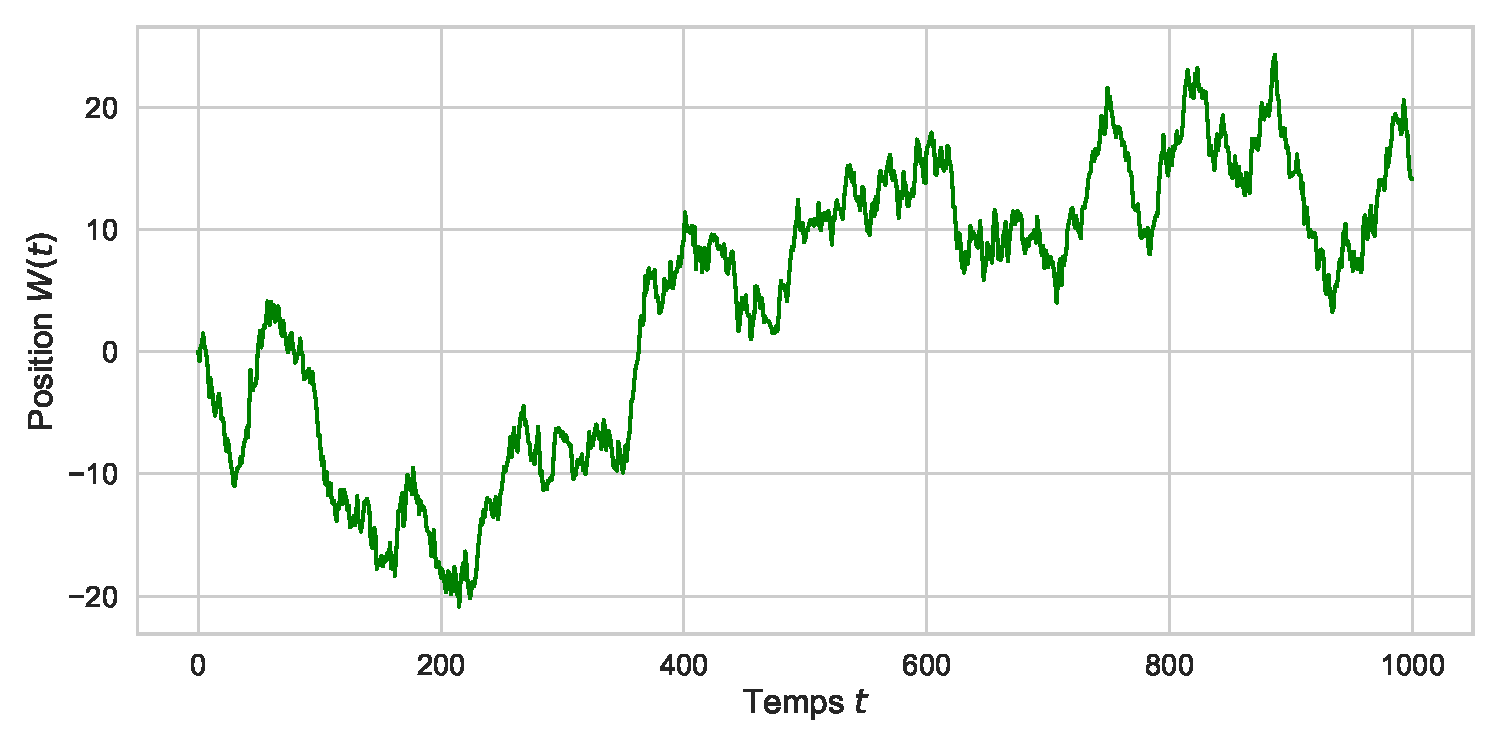
\includegraphics[width=0.9\linewidth]{img/intro/path_MBS.pdf}
    \caption{Une trajectoire du \acl{MBS}}\label{fig:TrajMBS}
\end{figure}
\FloatBarrier Le \acs{MBS} constitue la base de la construction des processus de diffusion employés dans de nombreux domaines tels que la finance, la physique ou la biologie. Ces processus sont modélisés par des \acf{EDS}, qui consistent à enrichir le mouvement brownien en y ajoutant un terme de dérive et un terme de diffusion. Il en résulte une classe de processus dits \textit{d'Itô}.
\paragraph{Définition: Processus d'Itô}\mbox{}\\
$\{X(t),\;t \geq 0\}$ est un processus d'Itô~\cite{ito1944} s'il satisfait une équation différentielle stochastique de la forme:
\begin{equation}
    dX(t) = \mu(t, X(t))\,dt + \sigma(t, X(t))\,dW(t)
\end{equation}\label{ito_eq}
où:
\begin{itemize}
    \item $\mu(t, X(t))$ et $\sigma(t, X(t))$ sont des fonctions mesurables et adaptées à la filtration brownienne standard $\mathcal{F}_t=\sigma\{W(s),\;s\leq t\}$;
    \item $\mathds{P}\left( \int_0^T |\mu(s, X(s))|\,ds < +\infty \right) = 1$;
    \item $\mathds{P}\left( \int_0^T \sigma^2(s, X(s))\,ds < +\infty \right) = 1$.
\end{itemize}
Dans cette formulation, $\mu(t, X(t))$ est appelé le \textit{terme de dérive} et $\sigma(t, X(t))$ le \textit{terme de diffusion}.
\begin{figure}[htb]
    \centering
    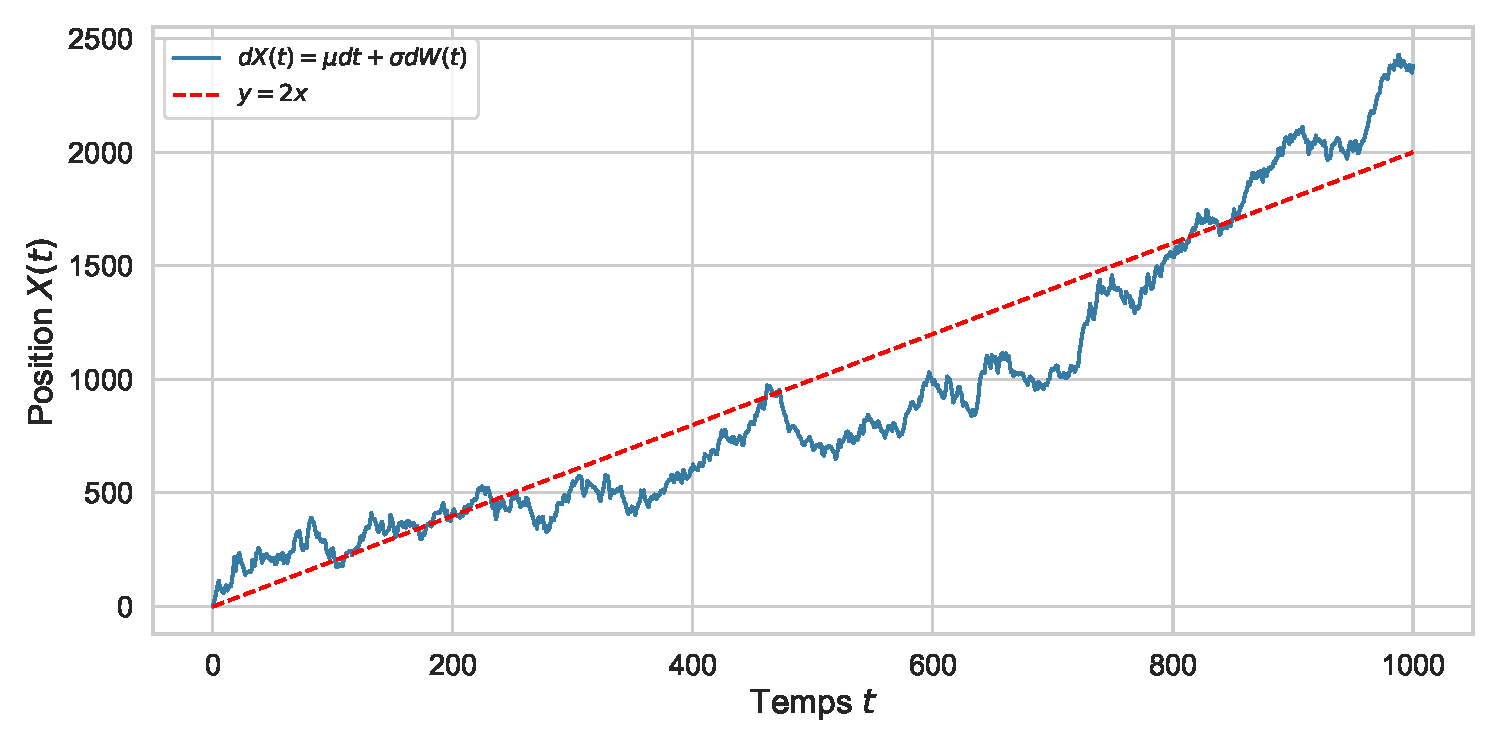
\includegraphics[width=0.9\linewidth]{img/intro/path_drift.pdf}
    \caption{Une trajectoire d'un processus d'Itô avec $\mu(t, X(t)) \equiv \mu = 2$}\label{fig:TrajIto}
\end{figure}
\FloatBarrier La figure~\ref{fig:TrajIto} illustre l'effet d'une dérive: la trajectoire du processus s'organise autour de la courbe moyenne \( y = 2x \), tout en étant perturbée par la composante aléatoire de la diffusion.

De plus, il est important de noter que les termes de dérive et de diffusion peuvent eux-mêmes dépendre de l'état du processus ou du temps, ce qui permet de capturer des dynamiques complexes, comme une volatilité ou une dérive variable. Cette flexibilité permet notamment de modéliser des phénomènes réalistes dans les systèmes financiers ou physiques.

Par ailleurs, Il est parfois intéressant d'enrichir les processus d'Itô en leur ajoutant une composante de sauts, gouvernée par un processus de Poisson (processus de comptage classique modélisant une file d'attente).
\paragraph{Définition: Processus de Poisson}\mbox{}\\
Un processus $\{N(t),\;t\geq0\}$ est un processus de Poisson de taux $\lambda$ s'il vérifie:
\begin{itemize}
    \item Pour des intervalles de temps disjoints, le nombre d'occurrences est indépendant: pour tout $0 \leq t_0 < t_1 < \cdots < t_n$, les variables aléatoires ${\left(N(t_i) - N(t_{i-1})\right)}_{i=1}^n$ sont indépendantes;
    \item La probabilité d'une occurrence dans un petit intervalle de temps dépend de la longueur de l'intervalle: $\underset{h\to0^+}{\lim}\mathds{P}[N(t+h)-N(t)=1]=\lambda h+o(h)$;
    \item La probabilité qu'il y ait plus d'une occurrence au sein d'un petit intervalle est négligeable: $\underset{h\to0^+}{\lim}\mathds{P}[N(t+h)-N(t)>1]=o(h)$;
    \item Le nombre d'occurrences dans un intervalle de longueur $t$ suit une loi poisson: $N(t)\sim \text{Poi}(\lambda t)$;
    \item Le temps d'arrivé du $n$-ème événement $T_n$ suis une loi exponentielle: $T_n\sim\text{Exp}(\lambda)$.
\end{itemize}
En utilisant un processus de Poisson, il est donc possible de définir un processus de sauts pur.
\paragraph{Définition: Processus de sauts purs}\mbox{}\\
Soit $\{N(t),\;t \geq 0\}$ un processus de Poisson de taux $\lambda > 0$ indépendant d'une suite de variables aléatoires indépendantes et identiquement distribuées $\{Y_i\}_{i \in \mathds{N}^*}$. On définit le processus de sauts purs $\{J(t),\;t \geq 0\}$ par:
\[
J(t) = \sum_{i=1}^{N(t)} Y_i
\]
Ce processus correspond à une somme aléatoire de sauts, où:
\begin{itemize}
    \item $N(t)$ représente le nombre de sauts survenus jusqu'au temps $t$;
    \item $Y_i$ est l'amplitude du $i$-ème saut;
    \item Les instants des sauts sont donnés par les temps d'arrivée du processus de Poisson;
    \item Entre deux sauts, le processus reste constant.
\end{itemize}
La figure ci-dessous visualise différentes réalisation d'un processus de sauts pur gouverné par un processus de Poisson de paramètre $\lambda=2$. La taille des sauts correspond à des réalisations d'une variable aléatoire exponentielle de paramètre $\nu=1.5$.
\begin{figure}[htb]
    \centering
    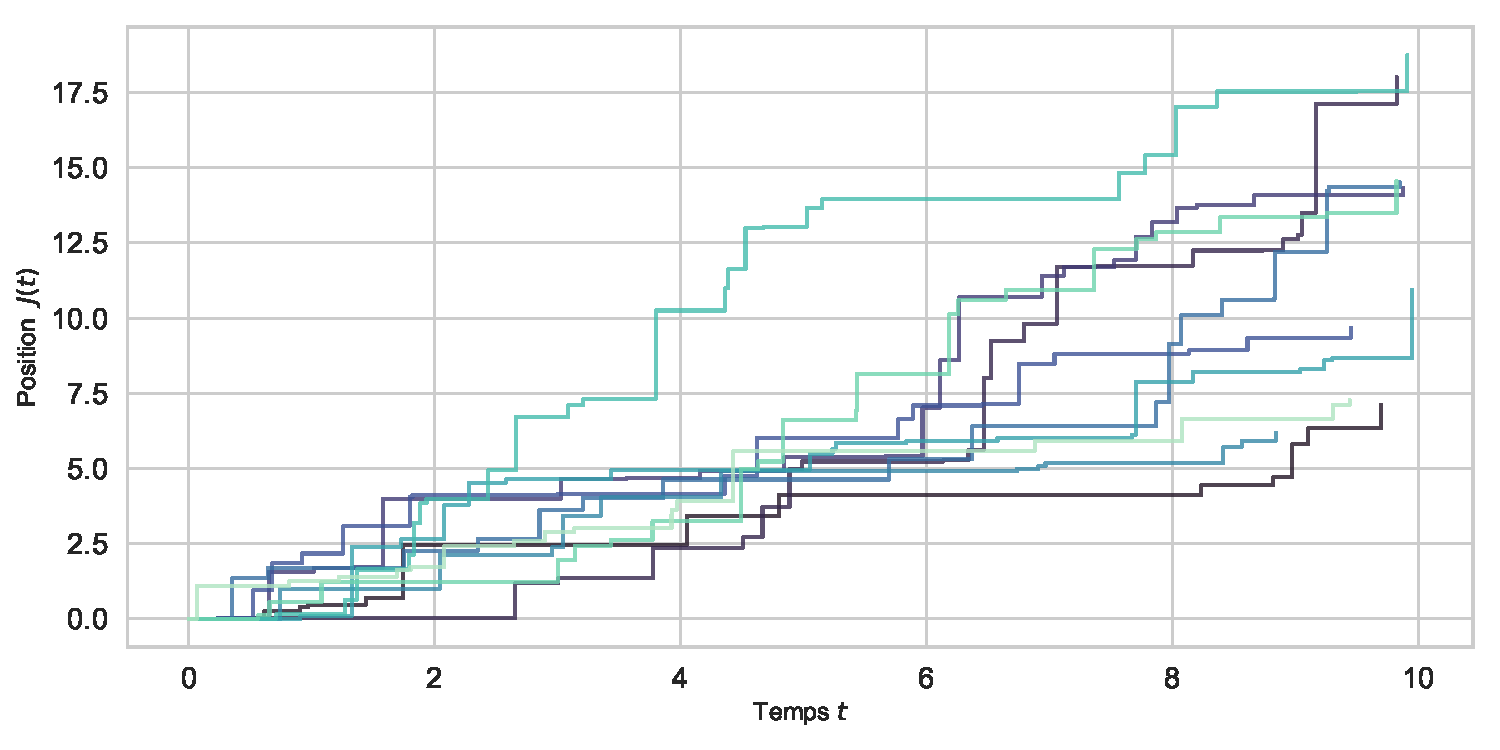
\includegraphics[width=0.9\linewidth]{img/intro/path_jump.pdf}
    \caption{Simulation de 10 trajectoire d'un processus de sauts pur $J(t)$}\label{fig:TrajJump}
\end{figure}
\FloatBarrier\clearpage

%%
%% ELEMENTS DE LA PROBLEMATIQUE
%%
\section{Éléments de la problématique}  % environ 3 pages

Comme évoqué précédemment, cette étude s'intéresse à des problèmes appliquées au processus \acl{CIR}. Il convient donc d'en donner une définition formelle.
\paragraph{Définition: Le processus \acl{CIR}}\mbox{}\\
Le processus \ac{CIR}~\cite{cox1985} est un processus d'Itô défini par l'équation différentielle stochastique suivante:
\begin{equation}
    dX(t) = a[b - X(t)]\,dt + \sigma \sqrt{X(t)}\,dW(t)
\end{equation}\label{cir_eq}
où:
\begin{itemize}
    \item $a \geq 0$ est le paramètre de vitesse;
    \item $b > 0$ représente la moyenne long-terme;
    \item $\sigma > 0$ est volatilité instantanée;
    \item $W(t)$ désigne un mouvement brownien standard.
\end{itemize}
Ce processus est particulièrement adapté à la modélisation des taux d'intérêt en raison de plusieurs propriétés clés:
\begin{itemize}
    \item Le terme de dérive $\mu(t, X(t)) \equiv \mu(X(t))= a[b - X(t)]$ induit un mécanisme de retour vers la moyenne $b$, avec une vitesse déterminée par $a$. Dans le contexte de modélisation des taux, cela reflète l'idée que ces derniers tendent à revenir vers un niveau de long terme après des déviations temporaires;
    \item Le terme de diffusion $\sigma(t, X(t))\equiv \sigma(X(t)) = \sigma \sqrt{X(t)}$ garantit la non-négativité du processus grâce à la racine carrée. Ceci est essentiel comme un taux négatif serait irréaliste dans de nombreux contextes économiques, en particulier pour les modèles de taux à court terme comme le CIR;
    \item Le comportement à proximité de zéro est gouverné par la \textit{condition de Feller}, selon laquelle:
    \[
    \mathds{P} \Big[ \exists\;t < \infty:X(t) = 0 \Big] = 1 \quad \text{si et seulement si} \quad \sigma^2 \geq 2ab
    \]
    Cela signifie que le processus peut atteindre zéro en un temps fini si la \textit{diffusion} domine la \textit{dérive}.
\end{itemize}
\begin{figure}[htb]
    \centering
    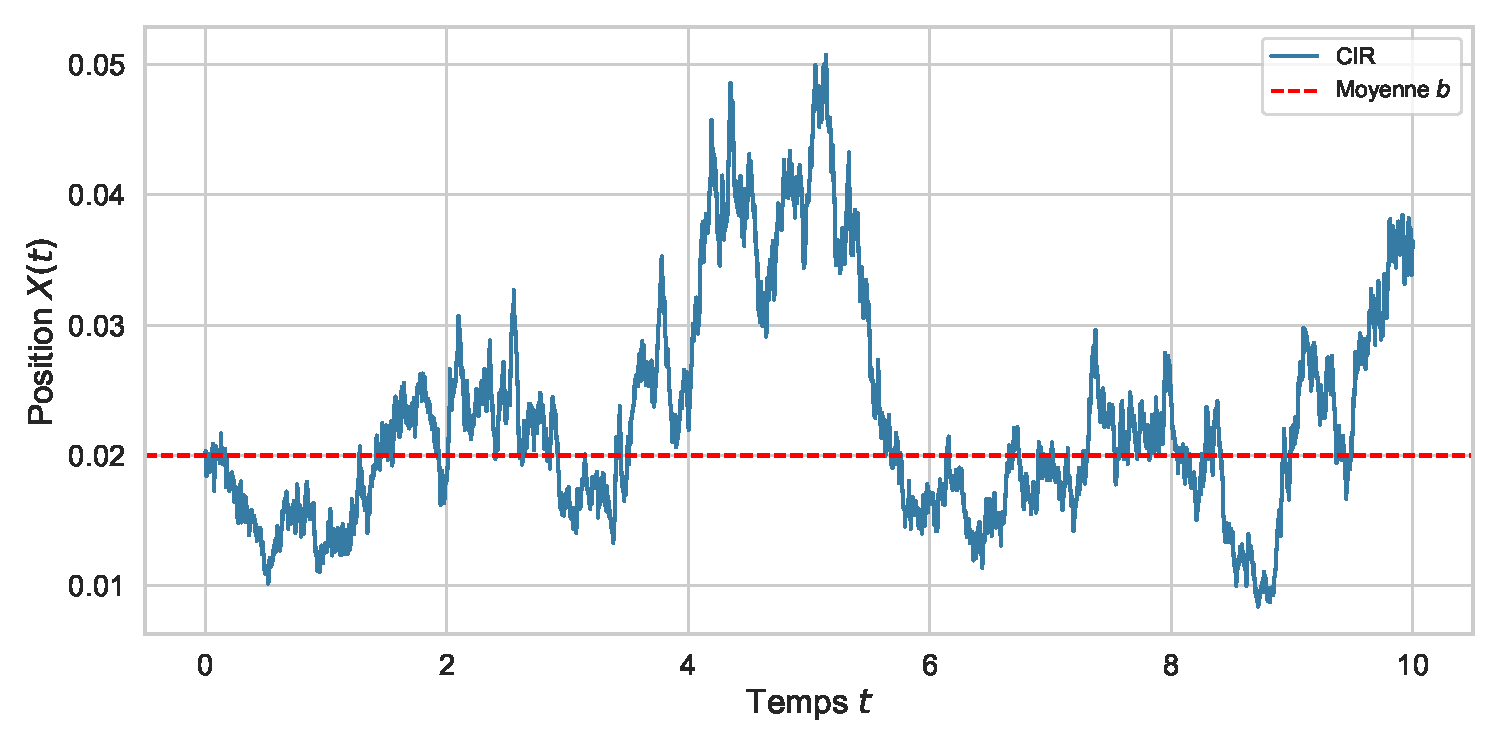
\includegraphics[width=0.9\linewidth]{img/intro/path_cir.pdf}
    \caption{Une trajectoire du processus \acs{CIR} avec $a=1$, $b=0.02$, $\sigma=0.1$}\label{fig:TrajCIR}
\end{figure}
\FloatBarrier Le prochain élément de problématique à introduire dans le cadre de cette étude est celui du \textit{temps de premier passage}.
\paragraph{Définition: Temps de premier passage}\mbox{}\\
Soit $\{X(t),\, t \geq 0\}$ un processus \acs{CIR}. Le \textit{temps de premier passage à deux frontières} est défini, pour un seuil $c > 0$, par:
\begin{equation}\label{fpt_definition}
    \tau(x) = \inf \left\{ t \geq 0: X(t) \notin (0, c) \,\middle|\, X(0) = x \in (0, c) \right\}
\end{equation}
Autrement dit, $\tau(x)$ correspond au premier instant où le processus atteint l'une des bornes de l'intervalle $(0, c)$. 

L'étude de ce temps d'arrêt est particulièrement pertinente dans le cadre du processus \acs{CIR}, pour plusieurs raisons:
\begin{itemize}
    \item \textbf{Modélisation du passage aux taux négatifs:} lors de la crise économique japonaise de 2016, des taux d'intérêt négatifs ont été instaurés pour stimuler l'activité. Or, le processus \acs{CIR}, à valeurs strictement positives, ne permet pas de modéliser ce phénomène. Introduire une barrière à zéro permet de considérer le franchissement de ce seuil, au-delà duquel les taux deviennent négatifs;
    \item \textbf{Surveillance des taux élevés:} en gestion des risques, il est crucial de modéliser l'éventualité d'une hausse brutale ou excessive des taux d'intérêt. L'introduction d'un seuil supérieur $c$ permet de caractériser ces situations critiques et de quantifier leur probabilité d'occurrence via le temps de franchissement.
\end{itemize}
\begin{figure}[htb]
    \centering
    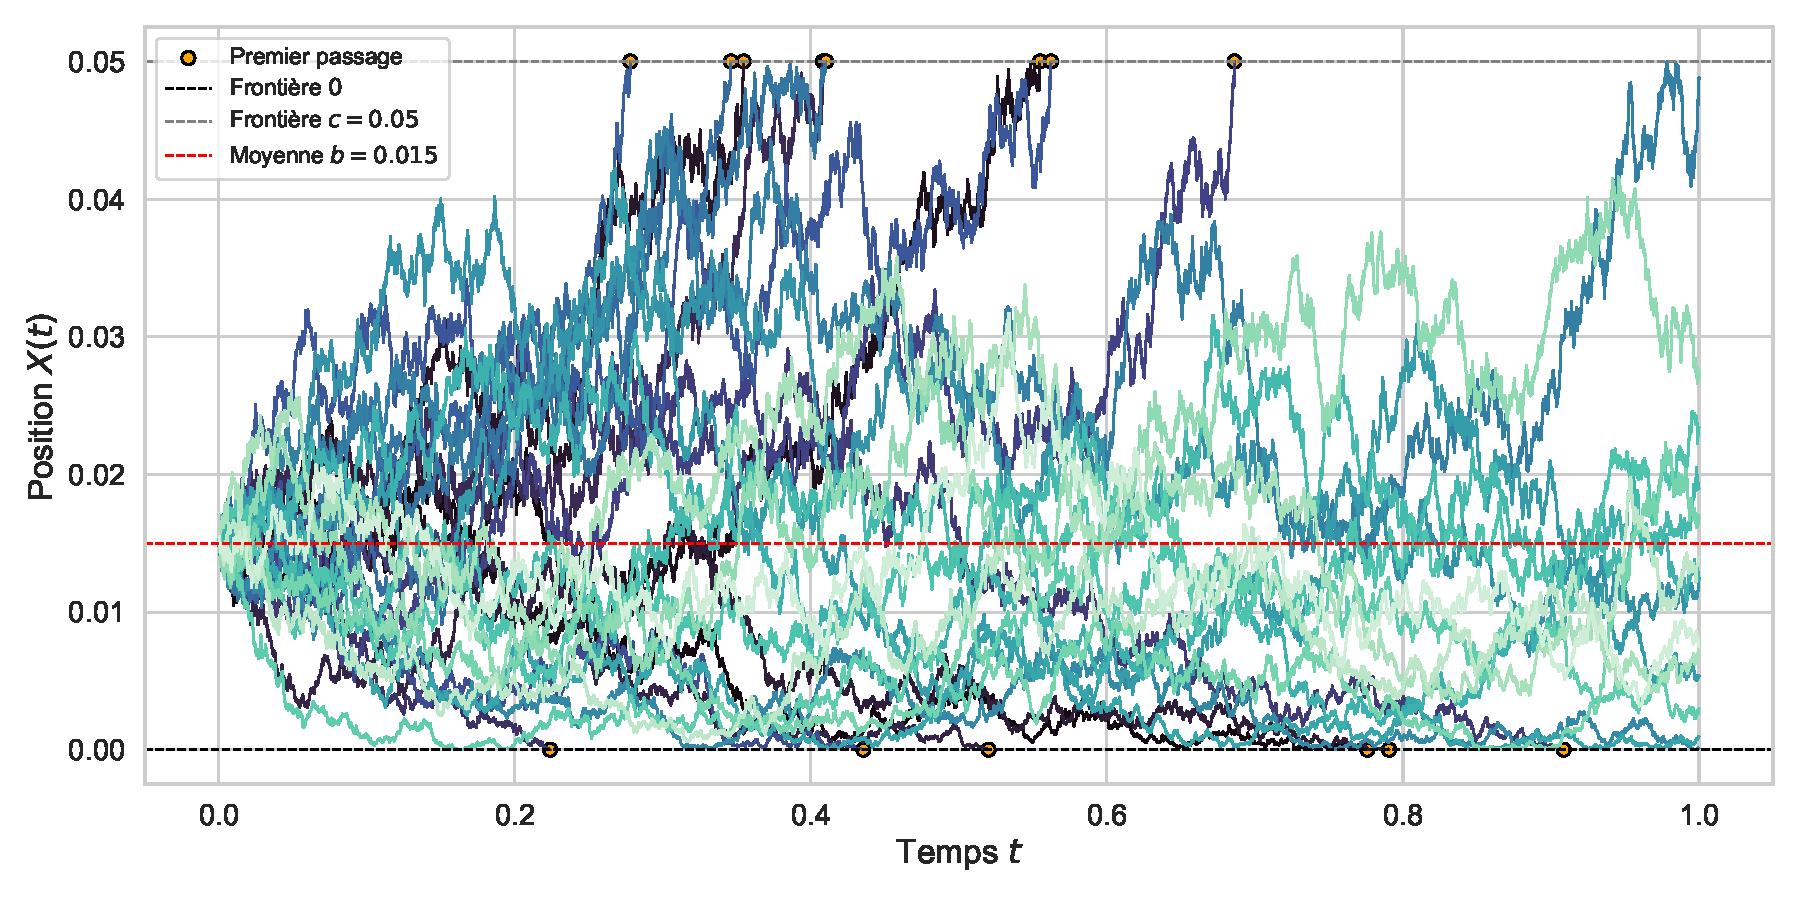
\includegraphics[width=0.9\linewidth]{img/intro/cir_first_passage.pdf}
    \caption{Simulations de 30 trajectoires du \acs{CIR} avec deux frontières absorbantes}\label{fig:FPTCIR}
\end{figure}
\FloatBarrier L'étude portera principalement sur le processus \acs{CIR}, noté $X(t)$, ainsi que sur la variable aléatoire associée au temps de premier passage $\tau(x)$.\\
Nous introduisons à présent les fonctions analytiques qui feront l'objet de l'analyse. La première est la \textit{fonction génératrice des moments}, outil central pour caractériser la distribution du temps d'arrêt.
\paragraph{Définition: \ac{FGM}}\mbox{}\\
La fonction génératrice des moments du temps de premier passage $\tau(x)$ est définie, pour tout $\alpha > 0$, par:
\begin{equation}\label{fgm}
    M(x;\alpha):= \mathds{E} \left[ e^{-\alpha \tau(x)} \right]
\end{equation}
Cette fonction permet de résumer l'information probabiliste sur la variable $\tau(x)$, en particulier sa distribution. De plus, elle encode l'ensemble des moments de $\tau(x)$, lorsque ceux-ci existent, via dérivation en $\alpha$. 

La deuxième fonction d'intérêt est celle du \textit{temps moyen de premier passage}, qui correspond à l'espérance de la variable aléatoire $\tau(x)$.
\paragraph{Définition: Temps Moyen de Premier Passage}\mbox{}\\
Le temps moyen de premier passage est défini par:
\begin{equation}\label{mean}
    m(x):= \mathds{E}[\tau(x)]
\end{equation}
Il représente le temps moyen que met le processus \acs{CIR}, partant d'un niveau initial $x \in (0,c)$, pour atteindre l'une des deux bornes de l'intervalle $(0,c)$.

La troisième fonction étudiée est celle de l'\textit{aire moyenne sous la trajectoire} jusqu'au temps de sortie.
\paragraph{Définition: Aire Moyenne}\mbox{}\\
La fonction d'aire moyenne est définie par:
\begin{equation}\label{area}
    A(x):= \mathds{E} \left[ \int_0^{\tau(x)} X(t)\,dt \right]
\end{equation}
En finance, l'aire moyenne peut représenter l'accumulation moyenne d'un taux d'intérêt à court terme jusqu'à un événement de sortie. Elle intervient également dans la tarification d'options asiatiques avec barrière, où le \textit{payoff} dépend de l'intégrale temporelle du sous-jacent avant la sortie d'un intervalle donné.

La quatrième fonction étudiée est celle de la \textit{probabilité toucher la frontière inférieure}.
\paragraph{Définition: Probabilité de Sortie en Zéro}\mbox{}\\
La fonction de probabilité de sortie est définie par:
\begin{equation}\label{zero_exit_probability}
    p(x):=\mathds{P}[X(\tau(x))=0]
\end{equation}
Elle caractérise la probabilité que le processus, partant d'une position initiale $x$, sorte de l'intervalle $(0,c)$ par le bas. Cette quantité peut être utilisée pour quantifier un risque de ruine, de défaut, ou encore d'apparition de taux négatifs (si le contexte économique le permet).

La cinquième fonction étudiée est celle du \textit{dépassement moyen}, en ajoutant des sauts au \acs{CIR}.
\paragraph{Définition: Dépassement Moyen}\mbox{}\\
La fonction dépassement moyen est définie par: 
\begin{equation}\label{overshoot}
    D(x)=\mathds{E}\left[(X(\tau(x))-c)_+\right]
\end{equation}
Elle quantifie le dépassement moyen au-dessus de la frontière \( c \), à partir d'une condition initiale \( X(0) = x \in (0, c) \). Il est essentiel de souligner que cette fonction ne présente un intérêt que dans le cas où le processus comporte des sauts. En effet, dans le cadre purement continu, la trajectoire atteint la frontière exactement, sans possibilité de la franchir.
\begin{figure}[htb]
    \centering
    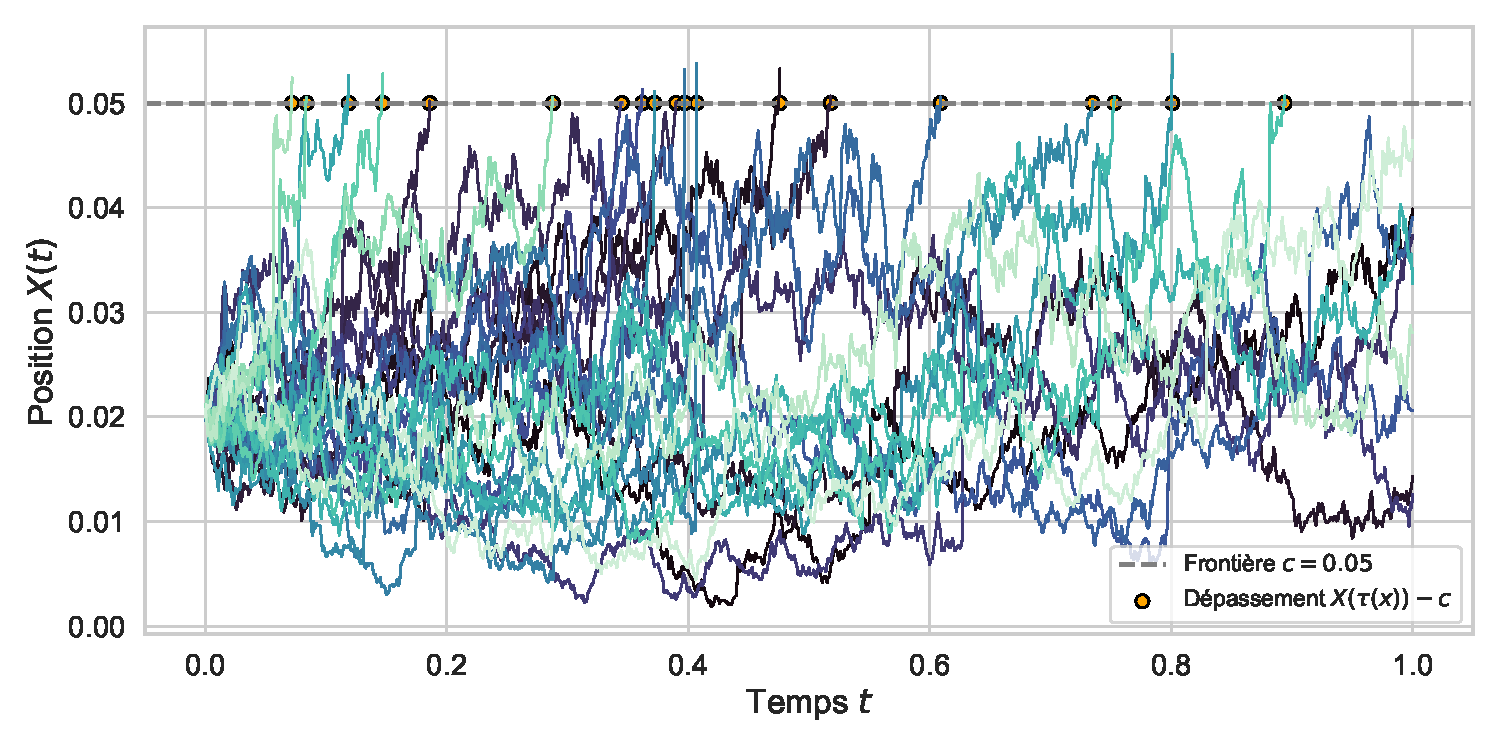
\includegraphics[width=0.9\linewidth]{img/intro/overshoot.pdf}
    \caption{Simulations de 30 trajectoires du \acs{CIR} avec sauts dépassants la frontière $c$}\label{fig:OvershootViz}
\end{figure}
\FloatBarrier Ce type de quantité apparaît notamment dans la valorisation de produits financiers path-dependent, tels que les options lookback ou les produits structurés à barrière, où le dépassement moyen modélise l'espérance de gain associée au franchissement d'un niveau critique par le sous-jacent. 

En complément de l'étude des temps de premier passage, ce mémoire s'intéresse également à un problème de \textit{commande optimale stochastique} appliqué au processus \acs{CIR}.
\paragraph{Définition: Problème de commande optimale \textemdash~Homing Problem}\label{definition_optimal_control}\mbox{}\\
Le \textit{Homing problem} consiste à piloter un processus stochastique dynamiquement jusqu'à ce qu'il atteigne un ensemble d'arrêt donné, tout en optimisant un objectif. La configuration étudiée dans ce mémoire correspond à un processus \acs{CIR} contrôlé \( \{X_u(t),\, t \geq 0\} \) évoluant dans l'intervalle \( (0, c) \), avec un arrêt déclenché dès que la trajectoire atteint l'une des deux frontières. Ce processus est défini par:
\begin{equation}\label{controlled_process}
    dX_u(t) = a[b - X_u(t)]dt + b[X_u(t)]u[X_u(t)]dt + \sigma \sqrt{X_u(t)} dW(t)
\end{equation}
où \( u(\cdot) \) est une stratégie de contrôle.

Le processus est contrôlé jusqu'à l'instant d'arrêt $\tau(x)$ défini précédemment (\ref{fpt_definition}).
Par ailleurs, l'objectif est de minimiser une fonction coût de type intégral, définie par:
\begin{equation}\label{cost_function}
    J(x) := \int_0^{\tau(x)} \left( \frac{1}{2}q[X_u(t)]u^2[X_u(t)] + r[X_u(t)] \right) dt
\end{equation}
où:
\begin{itemize}
    \item \( r(x) \neq 0 \) est le coût d'état (non associé au contrôle);
    \item \( b(x) \neq 0 \) est le coût du contrôle appliqué;
    \item \( q(x) > 0 \) est un poids pénalisant l'intensité du contrôle.
\end{itemize}
Le problème consiste à déterminer une stratégie optimale \( u^*(x) \) minimisant ce coût. La fonction valeur associée au problème s'écrit:
\begin{equation}\label{value_function}
    F(x) := \inf_{\underset{0 \leq t \leq \tau(x)}{u[X_u(t)]}} \mathds{E}[J(x)]
\end{equation}
La figure ci-dessous illustre l'effet d'une stratégie de contrôle sur la dynamique du processus. Dans cet exemple, la commande utilisée est constante et positive ($u(x)\equiv5$), ce qui génère une force dirigée vers la frontière supérieure \( c \) et accélère ainsi la sortie du processus par le haut.
\begin{figure}[htb]
    \centering
    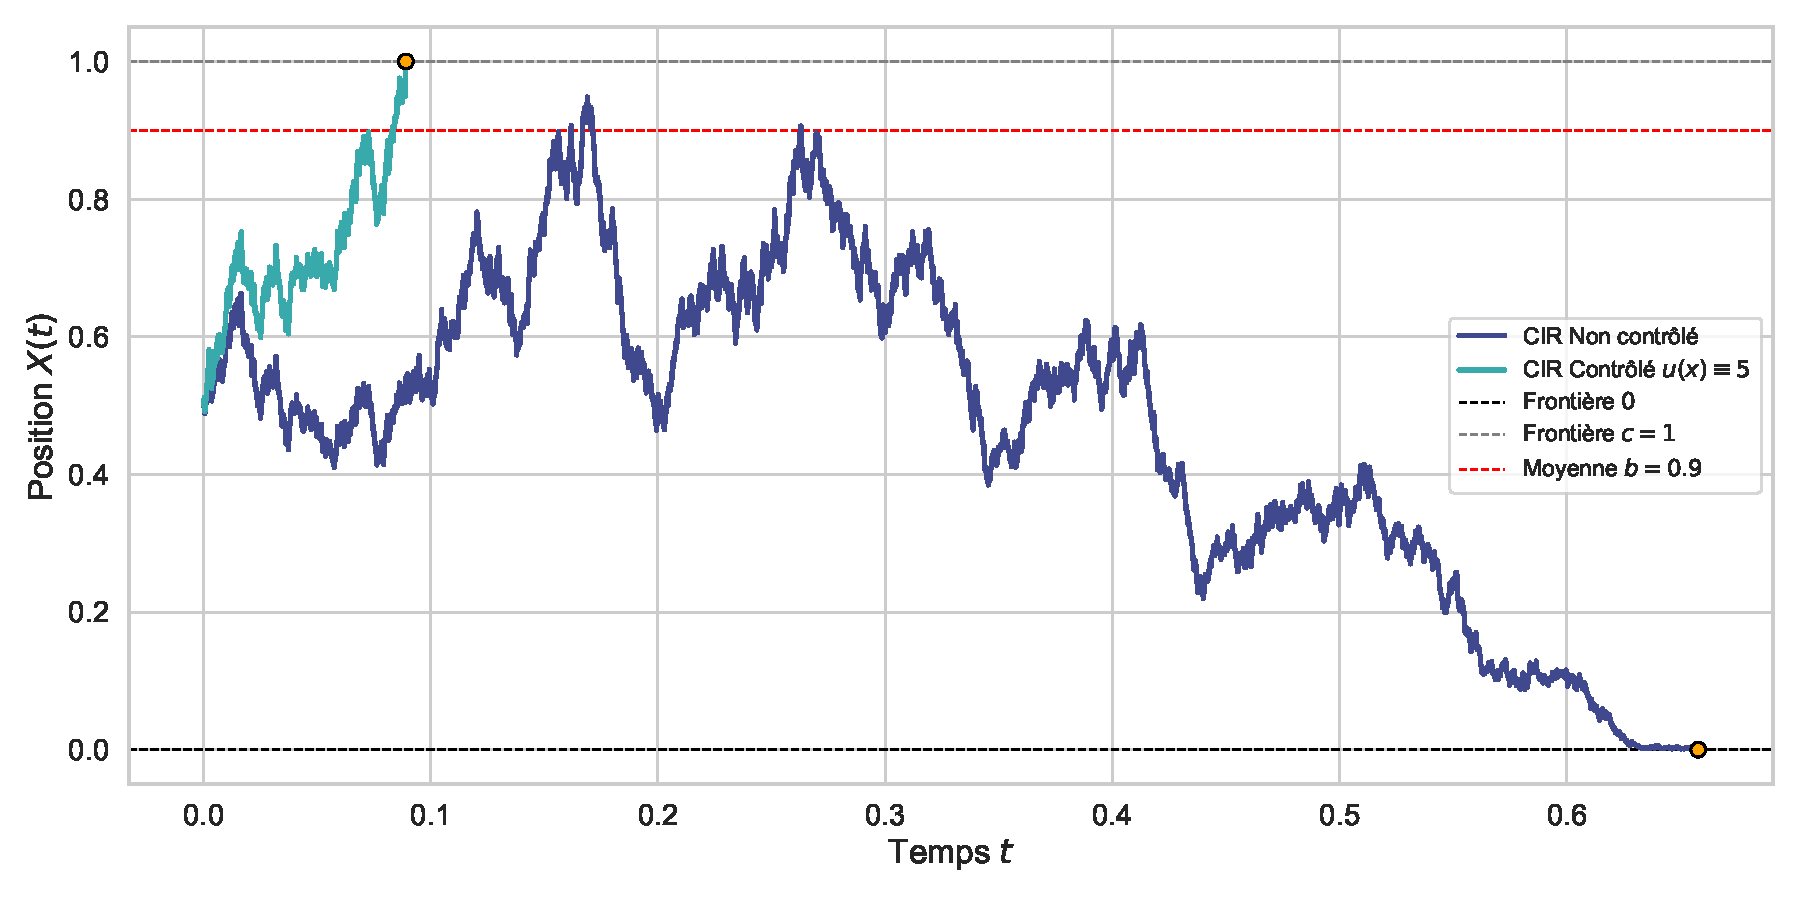
\includegraphics[width=0.9\linewidth]{img/intro/control.pdf}
    \caption{Simulations de deux trajectoires du CIR avec et sans contrôle}\label{fig:ControlViz}
\end{figure}
\FloatBarrier



\clearpage

%%
%% OBJECTIFS DE RECHERCHE / RESEARCH OBJECTIVES
%%
\section{Objectifs de recherche}  % 0.5 page

Après avoir exposé les fondements théoriques de l'étude, nous pouvons désormais énoncer précisément les objectifs poursuivis dans ce mémoire. Ceux-ci se répartissent en deux volets: l'analyse des temps de premier passage pour le processus \acs{CIR} en diffusion pure, puis l'étude de son extension avec sauts.
\paragraph{Objectifs pour le processus de diffusion}
\begin{itemize}
    \item Obtenir une expression explicite de la fonction génératrice des moments du temps de premier passage à deux frontières \( M(x;\alpha) = \mathds{E}[e^{-\alpha \tau(x)}] \);
    \item Expliciter une formule analytique pour le temps moyen de premier passage, \( m(x) = \mathds{E}[\tau(x)] \), pour une entrée initiale \( x \in (0,c) \);
    \item Déduire l'aire moyenne sous la trajectoire $A(x)$ jusqu'au franchissement de l'intervalle \( (0,c) \);
    \item Résoudre différentes formes d'un problème de commande optimale associé au processus, en déterminant la fonction valeur \( F(x) = \underset{u}{\inf}\,\mathds{E}[J(x)] \), ainsi que la politique de contrôle optimal $u^*(x)$.
\end{itemize}
\paragraph{Objectifs pour le processus de diffusion avec sauts}
\begin{itemize}
    \item Obtenir une expression analytique du temps moyen de sortie dans ce nouveau cadre, en tenant compte de l'impact des sauts sur la dynamique du processus;
    \item Établir une forme explicite de la probabilité de sortie par zéro:
    \(
    p(x) = \mathds{P}[X(\tau(x)) = 0],
    \)
    dans le cas de sauts uniformes descendants;
    \item Déterminer le dépassement moyen à l'instant du franchissement supérieur \( c \), défini par:
    \(
    D(x) = \mathds{E}[(X(\tau(x)) - c)_+]
    \)
    afin d'évaluer l'intensité des excursions au-delà de la borne supérieure, dans le cas de sauts exponentiels ascendants.
\end{itemize}


%%
%% PLAN DU MEMOIRE / THESIS OUTLINE
%%
\section{Plan du mémoire}  % 0.5 page
Afin de répondre aux objectifs de recherche définis précédemment, ce mémoire est structuré de la manière suivante.

Dans un premier temps, une revue de la littérature est proposée afin de replacer l'étude dans le cadre des travaux existants sur les temps de premier passage et les problèmes de dépassement, avec une attention particulière portée au processus \acs{CIR} et à ses extensions.

La suite du mémoire est consacrée à l'étude analytique des fonctions caractéristiques associées au processus. L'analyse se divise en trois parties distinctes: 
\begin{itemize}
    \item la première porte sur les problèmes de premier passage pour le processus \acs{CIR} en diffusion pure;
    \item la seconde examine sa version modifiée par l'introduction de sauts discrets;
    \item la troisième se consacre à l'étude de la commande optimale appliquée au \acs{CIR} diffusif.
\end{itemize}

Chaque section est accompagnée d'une analyse des résultats obtenus, permettant de vérifier la cohérence des solutions, d'en évaluer la sensibilité aux paramètres du modèle, et de comparer les dynamiques avec et sans sauts.

Enfin, la conclusion synthétise les contributions principales du mémoire, discute les limites de l'approche adoptée, et propose plusieurs pistes d'approfondissement pour des travaux futurs.

       % Introduction au sujet de recherche.
\Chapter{REVUE DE LITTÉRATURE}\label{sec:RevLitt}

Le problème du \textit{temps de premier passage} (\acs{TPP}) consiste à déterminer le moment où un processus stochastique atteint un seuil prédéfini pour la première fois. Ce concept joue un rôle central dans de nombreuses disciplines, notamment en physique, biologie, ingénierie, et particulièrement en mathématiques financières. Parmi les modèles les plus utilisés dans ce contexte, le processus de \ac{CIR}, également appelé processus racine-carrée de Feller (ou encore une transformation du processus de Bessel au carré), occupe une place importante en raison de sa propriété de non-négativité et de son comportement attractif autour d'une moyenne. Ce processus est notamment utilisé pour modéliser les dynamiques des taux d'intérêt.

Ce chapitre propose une synthèse des travaux existants sur les \acs{TPP} appliqués au processus \acs{CIR} (voir \cite{dinardo2021,dinardo2024,kepplinger2017,giorno2021,giorno2023,martin2011,masoliver2012}) ainsi que les problèmes de dépassement pour différents processus de diffusion (voir \cite{kou2003,yin2014,kluppelberg2004}), en mettant l'accent sur les méthodes analytiques, numériques et statistiques. L'objectif est de situer le présent mémoire dans l'état de l'art et de justifier les approches retenues par la suite.

\paragraph{Approche par cumulants et fonctions de Kummer}

Dans\cite{dinardo2021}, l'auteur développe une approche analytique du \acs{TPP} pour le processus \acs{CIR} en utilisant la transformée de Laplace de la densité de passage. Celle-ci s'exprime via la fonction hypergéométrique confluente de Kummer:
\[
\tilde{g}(z) = \frac{\Phi\left(\frac{z}{\tau}, s, \frac{2\tau(y_0-c)}{\sigma^2}\right)}{\Phi\left(\frac{z}{\tau}, s, \frac{2\tau(S-c)}{\sigma^2}\right)}, \quad z > 0.
\]
Les moments du \acs{TPP} sont ensuite obtenus à partir des cumulants, exprimés en fonction de polynômes logarithmiques et de nombres de Stirling. Cela permet, entre autres, de construire des développements en série à l'aide de polynômes de Bell. L'auteur propose également une approximation de la fonction de répartition à l'aide d'un développement en séries basé sur la densité Gamma et les polynômes de Laguerre.

\paragraph{Développement orthogonal basé sur la densité Gamma}

Dans\cite{dinardo2024}, cette approche est affinée par un développement tronqué de la densité du \acs{TPP}:
\[
g(t) \approx \hat{g}_n(t) = \frac{\beta {(\beta t)}^\alpha e^{-\beta t}}{\Gamma(\alpha+1)} \sum_{k=0}^n a_k^{(\alpha)} Q_k^{(\alpha)}(\beta t),
\]
où \( Q_k^{(\alpha)} \) sont des polynômes de Laguerre orthonormés, et \( a_k^{(\alpha)} \) des coefficients dépendant des moments. Cette méthode est accompagnée d'une analyse de convergence et d'un algorithme d'acceptation-rejet pour la simulation du \acs{TPP}.

\paragraph{Méthodes analytiques et intégrales de Volterra}

L'article\cite{kepplinger2017} traite le \acs{TPP} pour des processus de diffusion généraux en formulant une équation intégrale de Volterra du premier type. Pour le processus \acs{CIR}, l'auteur utilise un changement de mesure transformant le problème en celui du processus de Feller. Les moments sont ensuite dérivés à l'aide de la transformée de Laplace et des fonctions de Kummer.

\paragraph{Formules analytiques pour le processus de Feller}

Dans\cite{giorno2021}, les auteurs généralisent les résultats précédents à différents régimes de dérive du processus de Feller, en exprimant la densité du \acs{TPP} à travers la fonction de Kummer du second type \( \Psi \) ou la fonction de Bessel modifiée \( K_\nu \), selon la valeur du paramètre \( a \) (positif, nul ou négatif). Des expressions explicites pour la densité et l'espérance du \acs{TPP} sont fournies.

\paragraph{Comparaison avec les processus de Wiener et d'Ornstein-Uhlenbeck}

Dans\cite{giorno2023}, une comparaison est effectuée entre les comportements de \acs{TPP} pour les processus de Wiener, d'Ornstein-Uhlenbeck (OU) et de Feller. Pour chacun, la probabilité d'atteindre l'état zéro est analysée. Des formules explicites sont données pour la densité du \acs{TPP} avec absorption à zéro, et une étude asymptotique met en lumière les différences structurelles entre ces modèles.

\paragraph{Lien avec les processus de type Bessel}

L'article\cite{martin2011} s'intéresse à un processus de type Bessel gouverné par l'équation:
\[
dX_t = \left(\frac{nD}{X_t}\right) dt + \sqrt{2D}\, dW_t,
\]
présentant des similarités structurelles avec le processus \acs{CIR}. Selon le paramètre \( n \), le comportement au voisinage de zéro varie (absorbant, réfléchissant, ou entrée). Les auteurs proposent une résolution du problème de passage à l'aide de la théorie de Sturm-Liouville et des fonctions de Bessel, et obtiennent des densités de \acs{TPP} analytiques. Une validation par simulation de type Euler-Maruyama complète l'étude.

\paragraph{Temps de premier passage avec sauts}

Dans le cas de processus à sauts, le franchissement du seuil peut se faire par discontinuité, générant un dépassement (\textit{overshoot}) dont l'analyse complique considérablement le calcul du \acs{TPP}. Pour un processus de diffusion avec sauts doublement exponentiels, Kou et Wang\cite{kou2003} obtiennent des expressions fermées pour la transformée de Laplace du \acs{TPP} et de la distribution conjointe entre le temps de passage et l'overshoot. Ils montrent que l'overshoot est exponentiel conditionnellement à sa positivité, et que l'indépendance conditionnelle entre le \acs{TPP} et le dépassement peut être exploitée pour simplifier les calculs.

\paragraph{Extensions à des lois plus générales}

Yin et al.\cite{yin2014} généralisent ce cadre aux sauts suivant une loi mixte exponentielle, obtenant également des formules explicites pour la transformée de Laplace jointe du \acs{TPP} et de l'overshoot. Par ailleurs, Klüppelberg, Kyprianou et Maller\cite{kluppelberg2004} analysent le cas de processus de Lévy à queue lourde et dérivent une expression asymptotique explicite de l'overshoot conditionnellement au franchissement d'un niveau élevé. Ces résultats constituent les rares cas où des expressions analytiques sont disponibles, et fournissent un point de comparaison pour l'étude du processus de \acs{CIR} avec sauts.
  % Revue de littérature / Literature review
%\Chapter{DÉTAILS DE LA SOLUTION}\label{sec:Theme1}

Cette partie du mémoire est consacrée à la résolution analytique des équations associées aux différents objectifs formulés en introduction (\ref{sec:Introduction}).

\section{Diffusion pure}
D'abord, le processus \acs{CIR} sous forme de diffusion pure est considéré. 
\subsection{Fonction Génératrice des Moments}\label{subsection_fgm_eq}
\paragraph{Dérivation de l'équation à résoudre}\phantom{}\\
Soit un processus d'Itô défini par l'\ac{EDS} (\ref{ito_eq}).
Il est connu que la \acl{FGM} d'un temps de premier passage $\tau(x)$ satisfait l'équation du passé de Kolmogorov (voir~\cite{cox2017} ou~\cite{lefebvre2007}): 
\[
\frac{1}{2}\sigma{(t,x)}^2M''(x;\alpha)+\mu(t,x)M'(x;\alpha)-\alpha M(x;\alpha)=0
\]
avec $M(0;\alpha)=M(c;\alpha)=1$. 

En reprenant les termes de dérive et de diffusion du \acs{CIR} (\ref{cir_eq}), l'\ac{EDO} linéaire de second ordre à résoudre devient: 
\begin{equation}\label{ode_fgm}
    \frac{1}{2}\sigma^2xM''(x;\alpha)+a(b-x)M'(x;\alpha)-\alpha M(x;\alpha)=0
\end{equation}

\paragraph{Résolution}\phantom{}\\
D'abord, en multipliant les deux côtés par $2/\sigma^2$ l'équation ci-dessus (\ref{ode_fgm}) est mise sous forme canonique: 
\[
xM''(x;\alpha)-\left(\frac{2a}{\sigma^2}x-\frac{2ab}{\sigma^2}\right)M'(x;\alpha)-\frac{2\alpha}{\sigma^2} M(x;\alpha)=0
\]
Ensuite, un changement de variable $y=\beta x$ avec $M(x;\alpha)=G(y;\alpha)$ est introduit. L'équation devient: 
\[
yG''(y;\alpha)-\left(\frac{2a}{\sigma^2} \beta y - \frac{2ab}{\sigma^2}\right)G'(y;\alpha)-\beta\frac{2\alpha}{\sigma^2} G(y;\alpha) = 0
\]
Ce changement de variable a pour objectif de déterminer, en fonction des autres paramètres du problème, la valeur de $\beta$ qui permet de ramener l'équation à la forme générale de l'équation de Kummer (\ref{kummer_eq}): 
\begin{equation}\label{kummer_eq}
    xf''(x)-(x-\theta)f'(x)-s f(x)=0,\quad\quad \theta,s\in\mathds{R}
\end{equation}
dont la solution est connue. Pour ce faire, il faut que:
\[
\frac{2a}{\sigma^2} \beta=1\implies\beta=\frac{\sigma^2}{2a}
\]
L'équation devient:
\begin{equation}\label{kummer_eq2}
    yG''(y;\alpha)-\left(y-\frac{2ab}{\sigma^2}\right)G'(y;\alpha)-\frac{\alpha}{a}G(y;\alpha) = 0
\end{equation}
La solution générale de cette dernière (\ref{kummer_eq2}) est de la forme (voir~\cite{magnus1966}): 
\[G(y;\alpha) = C_1\Phi\left(\frac{\alpha}{a}, \frac{2ab}{\sigma^2}, y\right) + C_2\Psi\left(\frac{\alpha}{a}, \frac{2ab}{\sigma^2}, y\right)\]
avec $C_1$ et $C_2$ des constantes à déterminer, et $\Phi(\cdot, \cdot, \cdot)$ et $\Psi(\cdot, \cdot, \cdot)$ sont les fonctions hypergéométriques confluentes de première et seconde espèce (voir annexe~\ref{special_functions}).

Finalement, l'expression analytique de la \acs{FGM} de $\tau(x)$ est: 
\begin{equation}\label{sol_fgm}
    M(x;\alpha) = C_1\Phi\left(\frac{\alpha}{a}, \frac{2ab}{\sigma^2}, \frac{2ax}{\sigma^2}\right) + C_2\Psi\left(\frac{\alpha}{a}, \frac{2ab}{\sigma^2}, \frac{2ax}{\sigma^2}\right)
\end{equation}

\paragraph{Détermination des constantes}\phantom{}\\
Les conditions aux limites $M(0;\alpha)=M(c;\alpha)=1$ permettent de déterminer les deux constantes $C_1$ et $C_2$ en résolvant le système suivant:
\[
\begin{cases}
    C_1\Phi\left(\frac{\alpha}{a}, \frac{2ab}{\sigma^2}, 0\right) + C_2\Psi\left(\frac{\alpha}{a}, \frac{2ab}{\sigma^2}, 0\right) = 1 \\
C_1\Phi\left(\frac{\alpha}{a}, \frac{2ab}{\sigma^2}, \frac{2ac}{\sigma^2}\right) + C_2\Psi\left(\frac{\alpha}{a}, \frac{2ab}{\sigma^2}, \frac{2ac}{\sigma^2}\right) = 1
\end{cases}
\]
Il en découle les valeurs suivantes pour $C_1$ et $C_2$: 
\begin{equation}\label{fgm_constants}
    \begin{aligned}
        &C_1 = \frac{\Phi(\frac{\alpha}{a}, \frac{2ab}{\sigma^2}, 0)-\Psi(\frac{\alpha}{a}, \frac{2ab}{\sigma^2}, 0)}{\Phi(\frac{\alpha}{a}, \frac{2ab}{\sigma^2}, \frac{2ac}{\sigma^2})\Psi(\frac{\alpha}{a}, \frac{2ab}{\sigma^2}, 0)-\Psi(\frac{\alpha}{a}, \frac{2ab}{\sigma^2}, \frac{2ac}{\sigma^2})} \\
        &C_2 = \frac{\Phi(\frac{\alpha}{a}, \frac{2ab}{\sigma^2}, \frac{2ac}{\sigma^2})-1}{\Phi(\frac{\alpha}{a}, \frac{2ab}{\sigma^2}, \frac{2ac}{\sigma^2})\Psi(\frac{\alpha}{a}, \frac{2ab}{\sigma^2}, 0)-\Psi(\frac{\alpha}{a}, \frac{2ab}{\sigma^2}, \frac{2ac}{\sigma^2})}
    \end{aligned}
\end{equation}

\subsection{Fonction Temps Moyen}\label{subsection_mean_eq}

\paragraph{Dérivation de l'équation à résoudre}\phantom{}\\
En combinant le développement en série entière de l'exponentielle: 
\[
e^x=\sum_{k=0}^\infty\frac{x^k}{k!}
\]
et la définition de la \acl{FGM} (\ref{fgm}), il est possible d'écrire (en supposant que les moments de $\tau(x)$ existent et sont finis): 
\begin{equation}\label{taylor_fgm}
    \begin{aligned}
        M(x;\alpha)=\mathds{E}\left[e^{-\alpha \tau(x)}\right]&=\mathds{E}\left[\sum_{k=0}^\infty\frac{{(-\alpha\tau(x))}^k}{k!}\right] \\
        &= \sum_{k=0}^\infty\frac{{(-\alpha)}^k\mathds{E}\left[{\tau(x)}^k\right]}{k!}\\
        &=1-\alpha\mathds{E}[\tau(x)]+\frac{\alpha^2}{2}\mathds{E}\left[{\tau(x)}^2\right]-\ldots
    \end{aligned}
\end{equation}
En injectant (\ref{taylor_fgm}) dans l'équation (\ref{ode_fgm}), et en reprenant la définition (\ref{mean}), il découle l'\acs{EDO} linéaire de second ordre suivante: 
\begin{equation}\label{ode_mean}
    \frac{1}{2}\sigma^2xm''(x)+a(b-x)m'(x)=-1   
\end{equation}
avec $m(0)=m(c)=0$. En résolvant cette équation, une expression analytique de la fonction temps moyen est obtenue. 

\paragraph{Réduction d'ordre}\phantom{}\\
D'abord, afin d'alléger la notation, soit:
\begin{equation}\label{notation}
\begin{cases}
    \alpha = \frac{2a}{\sigma^2} \\
    \beta=\frac{2ab}{\sigma^2} \\
    \theta=-\frac{2}{\sigma^2}
\end{cases}
\end{equation}
L'équation peut donc être réécrite comme suit: 
\begin{equation}\label{simplified_ode_mean}
    xm''(x)+(\beta-\alpha x)m'(x)=\theta
\end{equation}
La réduction d'ordre $u(x)=m'(x)$ donne l'\acs{EDO} linéaire de premier ordre suivante:
\begin{equation}\label{order_reduction}
xu'(x)+(\beta-\alpha x)u(x)=\theta
\end{equation}
Pour procéder à sa résolution, il faut résoudre l'équation homogène associée puis déduire une solution particulière avec la méthode de variation de la constante. La solution générale obtenue est, avec $C_1$ une constante: 
\begin{equation}\label{sol_first_order_mean}
    u(x)=x^{-\beta}e^{\alpha x}(C_1-\theta \alpha^{-\beta}\Gamma(\beta, \alpha x))
\end{equation}
où $\Gamma(\cdot,\cdot)$ est la fonction Gamma incomplète (voir annexe~\ref{special_functions}).
Il suffit donc d'intégrer $u(x)$ et d'ajouter une constante $C_2$ pour obtenir l'expression de $m(x)$: 
\begin{equation}\label{intergration_sol_first_order}
    m(x)=\int u(x)dx+C_2
\end{equation}
Cependant, un problème survient lors de l'intégration du terme:
\begin{equation}\label{problematic_integral}
    \int\theta \underbrace{\phantom{|}{(\alpha x)}^{-\beta}\phantom{|}}_{P}\underbrace{\phantom{|}e^{\alpha x}\phantom{|}}_{E}\underbrace{\phantom{|}\Gamma(\beta, \alpha x)\phantom{|}}_{G}dx
\end{equation}
dans l'expression de $u(x)$ donnée par (\ref{sol_first_order_mean}). En effet, cette intégrale ne possède pas de solution analytique. Les logiciels de calcul symbolique tels que \textit{Mathematica} ou \textit{Maple} échouent également à en trouver une. Il est donc nécessaire d'explorer une autre approche afin de contourner cette difficulté.
\paragraph{Intégration}\phantom{}\\
L'intégrande de (\ref{problematic_integral}) présente des difficultés en raison de la présence du terme puissance $P:={(\alpha x)}^{-\beta}$ multiplié par le terme $E:=e^{\alpha x}$, ainsi que le terme $G:=\Gamma(\beta, \alpha x)$ (lui-même une intégrale). L'objectif est donc de reformuler cette expression afin de simplifier ou d'éliminer certains termes problématiques. C'est précisément ce qui sera abordé dans la suite de cette section. En effet, en combinant les deux expressions suivantes~\cite{NIST:DLMF}: 
\begin{align*}
    \left\{
    \begin{aligned}
        \Gamma(s,x) &= \Gamma(s)-\gamma(s,x) \\
        \gamma(s,x) &= x^s\Gamma(s)e^{-x}\sum_{k=0}^{\infty} \frac{x^k}{\Gamma(s+k+1)}
    \end{aligned}
    \right.
\end{align*}
avec $\gamma(\cdot,\cdot)$ une autre forme de la fonction gamma incomplète (voir annexe~\ref{special_functions}). 

Il est possible d'écrire:
\[
    \Gamma(s,x) = \Gamma(s)-x^s\Gamma(s)e^{-x}\sum_{k=0}^{\infty} \frac{x^k}{\Gamma(s+k+1)}
\]
et donc, en reprenant les termes de l'équation à résoudre (\ref{notation}) il découle l'expression suivante: 
\begin{equation}\label{incomplete_gamma_simplification}
    \Gamma(\beta, \alpha x) = \Gamma(\beta)-\Gamma(\beta)\underbrace{\phantom{|}{(\alpha x)}^\beta\phantom{|}}_{P'} \underbrace{\phantom{|}e^{-\alpha x}\phantom{|}}_{E'}\sum_{k=0}^{\infty} \frac{{(\alpha x)}^k}{\Gamma(\beta+k+1)}
\end{equation}
L'expression ci-dessus (\ref{incomplete_gamma_simplification}) est très intéressante. En effet, en remplaçant le terme $G$ dans (\ref{problematic_integral}) par (\ref{incomplete_gamma_simplification}), les termes $P$ et $P'$ ainsi que $E$ et $E'$ se simplifient comme suit:
\[
    \begin{aligned}
        &\int\theta \underbrace{\phantom{|}{(\alpha x)}^{-\beta}\phantom{|}}_{P}\underbrace{\phantom{|}e^{\alpha x}\phantom{|}}_{E}\overbrace{\left(\Gamma(\beta)-\Gamma(\beta)\underbrace{\phantom{|}{(\alpha x)}^\beta\phantom{|}}_{P'} \underbrace{\phantom{|}e^{-\alpha x}\phantom{|}}_{E'}\sum_{k=0}^{\infty} \frac{{(\alpha x)}^k}{\Gamma(\beta+k+1)}\right)}^{G}dx \\
        &= \int\theta\Gamma(\beta)\underbrace{\phantom{|}{(\alpha x)}^{-\beta}\phantom{|}}_{P}\underbrace{\phantom{|}e^{\alpha x}\phantom{|}}_{E}dx-\int\theta\Gamma(\beta)\underbrace{\phantom{|}{(\alpha x)}^{-\beta}\phantom{|}}_{P}\underbrace{\phantom{|}{(\alpha x)}^\beta\phantom{|}}_{P'}\underbrace{\phantom{|}e^{\alpha x}\phantom{|}}_{E} \underbrace{\phantom{|}e^{-\alpha x}\phantom{|}}_{E'}\sum_{k=0}^{\infty} \frac{{(\alpha x)}^k}{\Gamma(\beta+k+1)} \\
        &= \int\theta\Gamma(\beta)\underbrace{\phantom{|}{(\alpha x)}^{-\beta}\phantom{|}}_{P}\underbrace{\phantom{|}e^{\alpha x}\phantom{|}}_{E}dx-\theta\Gamma(\beta)\int\sum_{k=0}^{\infty} \frac{{(\alpha x)}^k}{\Gamma(\beta+k+1)}
    \end{aligned}
\]
En injectant dans (\ref{intergration_sol_first_order}), il découle: 
\[
m(x)=(C_1-\theta\alpha^{-\beta}\Gamma(\beta))\underbrace{\int x^{-\beta}e^{\alpha x}dx}_I + \,\theta\Gamma(\beta) \underbrace{\int\sum_{k=0}^{\infty} \frac{{(\alpha x)}^k}{\Gamma(\beta+k+1)}dx}_J + C_2
\]
avec $I$ et $J$ deux intégrales à résoudre: 
\begin{itemize}
    \item \textbf{Résolution de} $I$: \\
    \textit{Wolfram Mathematica} donne:
    \begin{equation}\label{exponential_integral}
        \int x^{-\beta}e^{\alpha x}dx = -x^{1-\beta}E_\beta(-\alpha x)
    \end{equation}
    où $E_n(x)$ est la fonction intégrale exponentielle généralisée (voir annexe~\ref{special_functions}).
    La relation suivante~\cite{abramowitz1964}:
    \[
    E_n(x)=x^{n-1}\Gamma(1-n,x)
    \]
    permet d'écrire: 
    \begin{equation}\label{exponential_integral_simplification}
        E_{\beta}(-\alpha x)={(-\alpha x)}^{\beta-1}\Gamma(1-\beta,-\alpha x)
    \end{equation}
    En combinant (\ref{exponential_integral}) et (\ref{exponential_integral_simplification}), l'expression analytique de la solution de $I$ est obtenue:
    \[
        I=-{(-\alpha)}^{\beta-1}\Gamma(1-\beta,-\alpha x)
    \]
    \item \textbf{Résolution de $J$}: \\
    La série à l'intérieur de l'intégrale converge uniformément grâce au terme factoriel au dénominateur. L'intégration terme-à-terme est donc possible: 
    \[
    \begin{aligned}
        \int\sum_{k=0}^{\infty} \frac{{(\alpha x)}^k}{\Gamma(\beta+k+1)}dx &= \sum_{k=0}^{\infty} \int \frac{{(\alpha x)}^k}{\Gamma(\beta+k+1)}dx \\
        &= \sum_{k=0}^{\infty} \frac{\alpha^k x^{k+1}}{(k+1)\Gamma(\beta+k+1)} \\
        &= \frac{x}{\Gamma(1+\beta)}\,_2F_2\left(\begin{bmatrix}1\\1\end{bmatrix},\begin{bmatrix}2\\1+\beta\end{bmatrix},\alpha x\right)
    \end{aligned}
    \]
    où $_p F_q(\cdot,\cdot,\cdot)$ est la fonction hypergéométrique généralisée (voir annexe~\ref{special_functions}).
    
\end{itemize}
La forme finale de l'expression de la fonction temps moyen est donc:
\begin{equation}\label{sol_mean}
    m(x)={(-\alpha)}^{\beta-1}\Gamma(1-\beta,-\alpha x)\left[\theta\alpha^{-\beta}\Gamma(\beta)-C_1\right]+\frac{\theta x}{\beta}\,{}_2F_2\left(\begin{bmatrix}1\\1\end{bmatrix},\begin{bmatrix}2\\1+\beta\end{bmatrix},\alpha x\right) + C_2
\end{equation}

\paragraph{Détermination des constantes}\phantom{}\\
Les conditions aux limites $m(0)=m(c)=0$ permettent de déterminer les deux constantes $C_1$ et $C_2$ en résolvant le système suivant: 
\begin{align*}
\left\{\begin{aligned}
(\theta\alpha^{-\beta}\Gamma(\beta)-C_1)\alpha^{\beta-1}\Gamma(1-\beta) + C_2 &= 0\\
(\theta\alpha^{-\beta}\Gamma(\beta)-C_1)\alpha^{\beta-1}\Gamma(1-\beta,\alpha c) + \frac{c\theta}{\beta}\,{}_2F_2\left(\begin{bmatrix}1\\1\end{bmatrix},\begin{bmatrix}2\\1+\beta\end{bmatrix},\alpha c\right)+ C_2 &= 0
\end{aligned}\right. \\
\end{align*}
Les expressions des constantes $C_1$ et $C_2$ sont donc:
\begin{equation}\label{mean_constants}
    \begin{aligned}
        C_1 &= \alpha^{-\beta}\theta\Gamma(\beta)+\frac{\alpha c \theta {(-\alpha)}^{-\beta}}{\beta\gamma(1-\beta,\alpha c)}\,{}_2F_2\left(\begin{bmatrix}1\\1\end{bmatrix},\begin{bmatrix}2\\1+\beta\end{bmatrix},\alpha c\right) \\
        C_2 &= -\frac{c\theta\Gamma(1-\beta)}{\beta\gamma(1-\beta,\alpha c)}\,{}_2F_2\left(\begin{bmatrix}1\\1\end{bmatrix},\begin{bmatrix}2\\1+\beta\end{bmatrix},\alpha c\right)
    \end{aligned}
\end{equation}
avec $\alpha$, $\beta$ et $\theta$ définis en (\ref{notation}).

\subsection{Fonction Aire Moyenne}

\paragraph{Dérivation de l'équation à résoudre}\phantom{}\\
Il est connu que l'\acs{EDO} de second ordre régissant la fonction (\ref{area}) est (voir~\cite{abundo2013}): 
\[\frac{1}{2}\sigma^2xA''(x)+a(b-x)A'(x)=-x\]
En reprenant les notations introduites en (\ref{notation}), l'équation devient: 
\[xA''(x)+(\beta-\alpha x)A'(x)=\theta x\]
Il convient de noter que cette équation ressemble beaucoup à celle dérivée en (\ref{simplified_ode_mean}). La résolution se fera donc de manière semblable.
\paragraph{Réduction d'ordre}\phantom{}\\
En procédant de façon identique à la résolution de l'équation du temps moyen (\ref{order_reduction},~\ref{sol_first_order_mean},~\ref{intergration_sol_first_order}), il est possible d'écrire: 
\[xu'(x)+(\beta-\alpha x)u(x)=\theta x\]
et donc: 
\[u(x)=C_1x^{-\beta} e^{\alpha x} -\theta\alpha^{-\beta-1}x^{-\beta} e^{\alpha x}\Gamma(\beta+1, \alpha x)\]
En combinant l'expression dérivée précédemment (\ref{incomplete_gamma_simplification}) et l'identité suivante~\cite{NIST:DLMF}: 
\[\Gamma(s+1, x)=s\Gamma(s, x)+x^s e^{-x}\]
il est possible de réécrire la solution sous la forme: 
\[
u(x)=C_1x^{-\beta} e^{\alpha x} -\theta\alpha^{-\beta-1}\left(\beta x^{-\beta}e^{\alpha x}\Gamma(\beta)\left(1-{(\alpha x)}^\beta e^{-\alpha x}\sum_{k=0}^{\infty} \frac{{(\alpha x)}^k}{\Gamma(\beta+k+1)}\right)+1\right)
\]

\paragraph{Intégration}\phantom{}\\
Pour obtenir la forme explicite de $A(x)$, il suffit d'intégrer $u(x)$ et d'ajouter une deuxième constante:
\[
\begin{aligned}
    A(x) &= \int u(x)dx+C_2 \\
    &= (C_1-\theta\alpha^{-\beta-1}\Gamma(\beta+1))\underbrace{\int x^{-\beta}e^{\alpha x}dx}_I +\frac{\theta\beta\Gamma(\beta)}{\alpha}\underbrace{\int\sum_{k=0}^{\infty} \frac{{(\alpha x)}^k}{\Gamma(\beta+k+1)}dx}_J-\theta\alpha^{-\beta-1}x +C_2 \\
\end{aligned}
\]
Les deux intégrales résolues précédemment $I$ et $J$ réapparaissent. En injectant leurs solutions, la forme finale de l'expression de la fonction Aire Moyenne est obtenue: 
\begin{equation}\label{sol_area}
    \begin{aligned}
            A(x) = {(-\alpha)}^{\beta-1}\Gamma(1-\beta,-\alpha x)[\theta\alpha^{-\beta-1}\Gamma(\beta+1)-C_1]\\+\frac{x\theta}{\alpha}\left[{}_2F_2\left(\begin{bmatrix}1\\1\end{bmatrix},\begin{bmatrix}2\\1+\beta\end{bmatrix},\alpha x\right)-\alpha^{-\beta}\right] +C_2 
    \end{aligned}
\end{equation}


\paragraph{Détermination des constantes}\phantom{}\\
Les conditions aux limites $A(0)=A(c)=0$ nous permettent de déterminer les deux constantes $C_1$ et $C_2$ en résolvant le système suivant: 
\begin{align*}
\left\{\begin{aligned}
    {(-\alpha)}^{\beta-1}\Gamma(1-\beta)(\theta\alpha^{-\beta-1}\Gamma(\beta+1)-C_1)+C_2 &= 0 \\
    {(-\alpha)}^{\beta-1}\Gamma(1-\beta,-\alpha c)[\theta\alpha^{-\beta-1}\Gamma(\beta+1)-C_1]\\+ \frac{c\theta}{\alpha}\left[{}_2F_2\left(\begin{bmatrix}1\\1\end{bmatrix},\begin{bmatrix}2\\1+\beta\end{bmatrix},\alpha c\right)-\alpha^{-\beta}\right] +C_2 &=0
\end{aligned}\right.
\end{align*}
Les constantes $C_1$ et $C_2$ s'écrivent donc: 
\begin{equation}\label{area_constants}
    \begin{aligned}
        C_1 =& \frac{1}{\gamma (1-\beta ,-\alpha c)}\Bigg[\theta  {(-\alpha)}^{-\beta } \alpha ^{-\beta -1} \Bigg\{c \alpha ^{\beta +1} \,{}_2F_2\left(\begin{bmatrix}1\\1\end{bmatrix},\begin{bmatrix}2\\1+\beta\end{bmatrix},\alpha c\right)\\&\quad\quad\quad\quad\quad\quad\quad\quad\quad\quad+
        {(-\alpha)}^{\beta } \Gamma(\beta +1)\gamma (1-\beta ,-c \alpha )-\alpha  c\Bigg\}\Bigg] \\
        C_2 =& -\frac{c \theta  \alpha ^{-\beta -1} \Gamma (1-\beta ) }{\gamma(1-\beta ,-c \alpha )}\left[\alpha ^{\beta } \,{}_2F_2\left(\begin{bmatrix}1\\1\end{bmatrix},\begin{bmatrix}2\\1+\beta\end{bmatrix},\alpha c\right)-1\right]
    \end{aligned}
\end{equation}

\subsection{Commande Optimale Stochastique}
Cette section est consacrée à l'étude du problème de commande optimale défini en (\ref{definition_optimal_control}).
\paragraph{Dérivation de l'équation de programmation dynamique}\phantom{}\\
En reprenant la définition (\ref{value_function}) et en appliquant le principe d'optimalité de Bellman, il découle:
\begin{equation}\label{Bellman_optimality}
        F(x) = \inf_u\mathds{E}\left[\int_0^{\delta t}\left(\frac{1}{2}q\left[X_u(s)\right]u^2\left[X_u(s)\right]+r\left[X_u(s)\right]\right)ds+F(X_u(\delta t))\right]
\end{equation}
D'une part, pour $\delta t$ petit, il est possible d'écrire:
\begin{equation}\label{cost_function_simplification}
    \int_0^{\delta t}\left(\frac{1}{2}q\left[X_u(s)\right]u^2\left[X_u(s)\right]+r\left[X_u(s)\right]\right)ds=\left(\frac{1}{2}q(x){u(x)}^2+r(x)\right)\delta t+o(\delta t)
\end{equation}
D'autre part, un développement de Taylor combiné avec la formule d'Itô~\cite{ito1944} (appliquée au processus contrôlé de dynamique (\ref{controlled_process})) permet d'écrire (en supposant que $F\in C^2$):
\begin{equation}\label{taylor_ito}
    \begin{aligned}
        \mathds{E}[F(X_u(\delta t))]&=F(x)+\mathds{E}[dF(X_u(\delta t))]+o(\delta t)\\
        &=F(x)+\mathds{E}\left[F'(X_u(\delta t))dX_u(t)+\frac{1}{2}F''(X_u(\delta t))d\langle X_u\rangle_{\delta t} \right]+o(\delta t)\\
        &=F(x)+\left[a(b-x)+b(x)u(x)\right]F'(x)\delta t+\frac{1}{2}\sigma^2xF''(x)\delta t+o(\delta t)
    \end{aligned}
\end{equation}
En injectant (\ref{cost_function_simplification}) et (\ref{taylor_ito}) dans (\ref{Bellman_optimality}), il découle:
\begin{equation}\label{initial_minimisation problem}
    \begin{aligned}
        F(x)&=\inf_u\Bigg\{\left(\frac{1}{2}q(x){u(x)}^2+r(x)\right)\delta t+F(x)+\left[a(b-x)+b(x)u(x)\right]F'(x)\delta t\\&\quad\quad\quad\quad\quad\quad\quad\quad\quad\quad\quad\quad\quad\quad\quad\quad\quad\quad\quad\quad+\frac{1}{2}\sigma^2xF''(x)\delta t+o(\delta t)\Bigg\}
    \end{aligned}
\end{equation}
Ensuite, en retranchant $F(x)$ des deux côtés, en divisant partout par $\delta t$ et en prenant la limite lorsque $\delta t\to0$, l'équation de programmation dynamique est obtenue:
\begin{equation}\label{minimisation_problem}
    0=\min_u\left\{r(x)+\frac{1}{2}q(x)u^2(x)+[a(b-x)+b(x)u(x)]F'(x)+\frac{1}{2}\sigma^2xF''(x)\right\}
\end{equation}
\paragraph{Détermination de la commande optimale et dérivation de l'équation associée}\phantom{}\\
La minimisation à faire dans (\ref{minimisation_problem}) est en fonction de $u(x)$. Le terme à minimiser est:
\[
f(u(x))=\frac{1}{2}q(x){u(x)}^2+b(x)u(x)F'(x)
\]
La minimisation donne:
\begin{equation}\label{optimal_control}
    \begin{aligned}
        f'(u^*(x))&=0\\
        q(x)u^*(x)+b(x)F'(x)&=0\\
    u^*(x)&=-\frac{b(x)}{q(x)}F'(x)
    \end{aligned}
\end{equation}
Par ailleurs, la dérivée seconde est: 
\[
f''(u(x))=q(x)\quad\forall\;u(x)
\]
Puisque \( q(x) > 0 \) par hypothèse (\ref{definition_optimal_control}), la dérivée seconde par rapport au contrôle est strictement positive. L'expression de \( u^*(x) \) obtenue en (\ref{optimal_control}) réalise donc bien un minimum global. Il s'agit ainsi du contrôle optimal.

En injectant ce dernier (\ref{optimal_control}) dans (\ref{minimisation_problem}), l'équation \acl{HJB} est obtenue, régissant la fonction valeur associée à la commande optimale:
\begin{equation}\label{control_equation}
    r(x) - \frac{{b(x)}^2}{2q(x)}{\left[F'(x)\right]}^2 + a(b - x)F'(x) + \frac{1}{2}\sigma^2 x F''(x) = 0
\end{equation}
avec $F(0)=F(c)=0$ et $r(x)\neq0, b(x)\neq0, q(x)>0$.


\subsubsection{Problème linéarisable}

Il faut donc procéder à la résolution de l'équation (\ref{control_equation}). Whittle~\cite{whittle1982} a montré que la transformation: 
\[F(x)=-K\log(\varphi(x))\]
avec $\varphi(0)=\varphi(c)=1$ permet de linéariser l'équation en posant:
\[
K=\frac{\sigma^2xq(x)}{{b(x)}^2}
\]
L'équation devient:
\begin{equation}\label{linearised_equation}
    \frac{1}{2}\sigma^2 x\varphi''(x) + a(b - x)\varphi'(x) - \frac{r(x)}{K}\varphi(x) = 0
\end{equation}
Dans le cas où le terme suivant est constant:
\begin{equation}\label{condition}
    \frac{r(x)}{K}\equiv k\in\mathds{R}\;\forall\;x
\end{equation}
l'équation (\ref{linearised_equation}) est identique à celle de la \acl{FGM} $M(x;\alpha)$ pour:
\[
\alpha=\frac{r(x)}{K}
\]
Cela permet de résoudre une multitude de problèmes en supposant différentes formes pour $r(x)$, $b(x)$ et $q(x)$ tout en satisfaisant la condition (\ref{condition}). 
Deux exemples de problèmes sont donnés dans les sous-parties suivantes.

\paragraph{Problème 1 \textemdash~P1}\label{p1}\phantom{}\\
\noindent Soit le problème suivant: 
\begin{itemize}
    \item $r(x) = \rho$: coût immédiat constant, indépendant de l'état $x$ et du contrôle.
    \item $b(x) = \beta x$: coût du contrôle proportionnel à $x$ sur la dynamique.
    \item $q(x) = \kappa x$: poids pénalisant l'intensité du contrôle, linéaire avec $x$.
\end{itemize}

Cela donne:
\[
K=\frac{\kappa \sigma^2}{\beta^2}
\]
L'équation devient:
\begin{equation}\label{eq_exemple1}
    \frac{1}{2}\sigma^2 x\varphi''(x) + a(b - x)\varphi'(x) - \frac{\rho\beta^2}{\kappa \sigma^2}\varphi(x) = 0
\end{equation}
La solution est:
\[
\varphi(x)=C_1\Phi\left(\frac{\rho\beta^2}{a\kappa \sigma^2},\frac{2ab}{\sigma^2},\frac{2ax}{\sigma^2}\right) + C_2\Psi\left(\frac{\rho\beta^2}{a\kappa \sigma^2},\frac{2ab}{\sigma^2},\frac{2ax}{\sigma^2}\right)
\]
Les conditions aux limites $\varphi(0)=\varphi(1)=1$ permettent de déterminer les constantes $C_1$ et $C_2$:
\begin{equation}\label{control_constants}
    \begin{aligned}
        C_1=\frac{\Psi\left(\frac{\beta ^2 \rho }{a \kappa  \sigma ^2},\frac{2 a b}{\sigma ^2},0\right)-\Psi\left(\frac{\beta ^2 \rho }{a \kappa  \sigma ^2},\frac{2 a b}{\sigma ^2},\frac{2 a c}{\sigma ^2}\right)}{\Psi\left(\frac{\beta ^2 \rho }{a \kappa  \sigma ^2},\frac{2 a b}{\sigma ^2},0\right) \, \Phi\left(\frac{\beta ^2 \rho }{a \kappa  \sigma ^2};\frac{2 a b}{\sigma ^2};\frac{2 a c}{\sigma ^2}\right)-\Psi\left(\frac{\beta ^2 \rho }{a \kappa  \sigma ^2},\frac{2 a b}{\sigma ^2},\frac{2 a c}{\sigma ^2}\right)} \\
        C_2= \frac{\, \Phi\left(\frac{\beta ^2 \rho }{a \kappa  \sigma ^2};\frac{2 a b}{\sigma ^2};\frac{2 a c}{\sigma ^2}\right)-1}{\Psi\left(\frac{\beta ^2 \rho }{a \kappa  \sigma ^2},\frac{2 a b}{\sigma ^2},0\right) \, \Phi\left(\frac{\beta ^2 \rho }{a \kappa  \sigma ^2};\frac{2 a b}{\sigma ^2};\frac{2 a c}{\sigma ^2}\right)-\Psi\left(\frac{\beta ^2 \rho }{a \kappa  \sigma ^2},\frac{2 a b}{\sigma ^2},\frac{2 a c}{\sigma ^2}\right)}
    \end{aligned}
\end{equation}
L'expression analytique de la fonction valeur est donc:
\begin{equation}\label{sol_control_1}
    F(x)=-\frac{\kappa \sigma^2}{\beta^2} \log\left[C_1\Phi\left(\frac{\rho\beta^2}{a\kappa \sigma^2},\frac{2ab}{\sigma^2},\frac{2ax}{\sigma^2}\right) + C_2\Psi\left(\frac{\rho\beta^2}{a\kappa \sigma^2},\frac{2ab}{\sigma^2},\frac{2ax}{\sigma^2}\right)\right]
\end{equation}
Par ailleurs, le contrôle optimal est
\begin{equation}\label{optimal_control_1}
    u^*(x)=-\frac{\beta}{\kappa}F'(x)
\end{equation}

\paragraph{Problème 2 \textemdash~P2}\label{p2}\phantom{}\\
\noindent Soit le problème suivant: 
\begin{itemize}
    \item $r(x) = \rho x$: coût immédiat linéaire en $x$, indépendant du contrôle.
    \item $b(x) = \beta \sqrt{x}$: coût du contrôle proportionnel à $\sqrt{x}$.
    \item $q(x) = \kappa x$: poids pénalisant l'intensité du contrôle, linéaire avec $x$.
\end{itemize}
Cela donne: 
\[
K=\frac{x\kappa \sigma^2}{\beta^2}
\]
L'équation obtenue est identique à celle du premier problème (\ref{eq_exemple1}): 
\[
\frac{1}{2}\sigma^2 x\varphi''(x) + a(b - x)\varphi'(x) - \frac{\rho\beta^2}{\kappa \sigma^2}\varphi(x) = 0
\]
L'expression de $\varphi(x)$ est donc la même. Il en découle alors l'expression de la solution $F(x)$: 
\begin{equation}\label{sol_control_2}
    F(x)=-\frac{x\kappa \sigma^2}{\beta^2}\left[C_1\Phi\left(\frac{\rho\beta^2}{a\kappa \sigma^2},\frac{2ab}{\sigma^2},\frac{2ax}{\sigma^2}\right) + C_2\Psi\left(\frac{\rho\beta^2}{a\kappa \sigma^2},\frac{2ab}{\sigma^2},\frac{2ax}{\sigma^2}\right)\right]
\end{equation}

Par ailleurs, le contrôle optimal est
\begin{equation}\label{optimal_control_2}
    u^*(x)=-\frac{\beta}{\kappa\sqrt{x}}F'(x)
\end{equation}

\subsubsection{Problème non linéarisable \textemdash~P3}\label{p3}
Soit le problème suivant:
\begin{itemize}
    \item $r(x) = x^2$: coût immédiat quadratique en $x$, indépendant du contrôle.
    \item $b(x) = x$: coût du contrôle linéaire égal à $x$.
    \item $q(x) \equiv 1$: poids pénalisant l'intensité du contrôle constant.
\end{itemize}
En éliminant le retour à la moyenne ($a=0$) et en posant $\sigma=1$, l'équation (\ref{control_equation}) se réduit à:
\begin{equation}\label{reduced_control_equation}
    x^2-\frac{x^2}{2}{F'(x)}^2+\frac{1}{2}xF''(x)=0
\end{equation}
Le logiciel de calcul symbolique \textit{Maple} donne comme solution pour $F(0)=0$ (avec $C_1$ une constante à déterminer):
\[
    F(x)=\int_0^x-\sqrt{2}\tanh\left(\frac{\sqrt{2}z^2}{2}+C_1\sqrt{2}\right)dz
\]
En posant $c=1$, la valeur de $C_1$ qui satisfait $F(c)=F(1)=0$ est $C_1\simeq -0.1652$. Donc, la forme finale de la fonction valeur est obtenue:
\begin{equation}\label{sol_control_3}
    F(x)\simeq \int_0^x-\sqrt{2}\tanh\left(\frac{\sqrt{2}z^2}{2}-0.1652\sqrt{2}\right)dz
\end{equation}
La commande optimale est donc:
\begin{equation}\label{optimal_control_3}
    u^*(x)\simeq x\sqrt{2}\tanh\left(\frac{\sqrt{2}x^2}{2}-0.1652\sqrt{2}\right)
\end{equation}

\section{Diffusion avec sauts}
Pour la suite, la variante discontinue du \acs{CIR} est portée à l'étude. Le processus est défini comme suit:
\begin{equation}\label{jump_cir_sde}
    X(t)=X(0)+\int_0^t a(b-X(s))ds+\int_0^t\sigma\sqrt{X(s)}dW(s)+J(t)
\end{equation}
avec
\begin{itemize}
    \item $X(0)=x$;
    \item $W(t)$ un \acs{MBS};
    \item $J(t)$ un processus de sauts pur:
    \[
    J(t)=\sum_{i=1}^{N(t)}Y_i
    \]
    où:
    \begin{itemize}
        \item $N(t)$ est un processus de poisson de paramètre $\lambda$;
        \item $Y_i$ des variables indépendantes et distribuées suivant une certaine loi.
    \end{itemize}
\end{itemize}

\subsection{Fonction Temps moyen \textemdash~Sauts uniformes}\label{subsection_mean_jumps}
Dans cette sous-section, la variante du \ac{CIR} avec sauts considérée est celle avec des sauts négatifs modélisés par des variables uniformément distribuées $Y_i\sim U[-x,0]$.

\paragraph{Dérivation de l'équation à résoudre}\phantom{}\\
En reprenant ce qui avait été fait en (\ref{subsection_fgm_eq}) pour dériver l'\acs{EDO} régissant la \acl{FGM} de $\tau(x)$ (voir, par exemple,~\cite{cox2017} ou~\cite{lefebvre2007}), il est possible d'écrire:
\[
\frac{1}{2}\sigma^2 xM''(x;\alpha)+a(b-x)M'(x;\alpha)+\lambda\left\{\frac{1}{x}\int_{-x}^0M(x+y;\alpha)dy-M(x;\alpha)\right\}-\alpha M(x;\alpha)=0
\]
avec $M(0;\alpha)=M(c;\alpha)=1$.

Ensuite, en procédant comme dans (\ref{subsection_mean_eq}), il découle l'équation du temps moyen de sortie de l'intervalle pour le processus avec sauts:
\begin{equation}\label{mean_ide}
    \frac{1}{2}\sigma^2 xm''(x)+a(b-x)m'(x)+\lambda\left\{\frac{1}{x}\int_{-x}^0m(x+y)dy-m(x)\right\}=-1
\end{equation}
avec $m(0)=m(c)=0$.

Soit le changement de variable suivant:
\begin{equation}\label{variable_change_mean}
    \int_{-x}^0m(x+y)dy=\int_0^x m(z)dz
\end{equation}
La formule de Leibniz permet d'écrire:
\[
\frac{d}{dx}\left(\int_0^x m(z)dz\right)=m(x)
\]
Donc, en dérivant les deux côtés de l'équation (\ref{mean_ide}) et en éliminant le retour à la moyenne ($a=0$), il découle une \acs{EDO} d'ordre 3:
\begin{equation}\label{mean_3rd_order}
    \frac{1}{2}\sigma^2xm'''(x)+\sigma^2m''(x)-\lambda m'(x)=-\frac{1}{x}
\end{equation}

\paragraph{Résolution}\phantom{}\\
Soit les valeurs suivantes des paramètres: $\sigma=\sqrt{2}$, $\lambda=1$ et $c=1$. \textit{Maple} donne comme solution:
\begin{equation}\label{sol_mean_with_jumps}
    m(x)=C_1I_0(2\sqrt{x})+C_2K_0(2\sqrt{x})+2\ln(2\sqrt{x})+C_3
\end{equation}
avec $C_1$, $C_2$, $C_3$ des constantes à déterminer et $I_0(\cdot)$, $K_0(\cdot)$ les fonctions de Bessel modifiées de première et seconde espèce respectivement (voir annexe~\ref{special_functions}).

Les constantes $C_1$, $C_2$ et $C_3$ sont déterminées en imposant les conditions aux limites $m(0)=m(1)=0$ ainsi qu'une condition supplémentaire $m(0.5)=r$. Ensuite, la valeur de $r$ permettant de satisfaire l'équation originale (\ref{mean_ide}) est trouvée: $r\simeq0.3281$.

\paragraph{Étude du cas sans sauts}\phantom{}\\
Afin de comparer l'effet de la présence des sauts, il est intéressant de résoudre le même problème en retirant ces derniers. Soit $m_0(x)$ le temps moyen de sortie du processus sans sauts. En considérant les mêmes valeurs des paramètres, l'équation à résoudre devient:
\begin{equation}\label{mean_3rd_order_without_jumps}
    xm_0''(x)=-1
\end{equation}
La solution qui satisfait $m_0(0)=m_0(1)=0$ est:
\begin{equation}\label{sol_mean_with_0_jumps}
    m_0(x)=-x\ln(x)
\end{equation}

\subsection{Fonction Probabilité de sortie en zéro \textemdash~Sauts uniformes}\label{subsection_probability_jumps}
Dans cette sous-section, la variante du \ac{CIR} avec sauts considérée est identique à la précédente (sauts négatifs modélisés par des variables uniformément distribuées $Y_i\sim U[-x,0]$).

\paragraph{Dérivation de l'équation à résoudre}\phantom{}\\
Il est possible de montrer que la fonction probabilité de sortie en zéro satisfait l'\acs{EDO}:
\begin{equation}\label{probability_ide}
    \frac{1}{2}\sigma^2xp''(x)+a(b-x)p'(x)+\lambda\left\{\frac{1}{x}\int_{-x}^0p(x+y)dy-p(x)\right\}=0
\end{equation}
sous les conditions $p(0)=1$ et $p(c)=0$.

Ensuite, en effectuant le même changement de variable que pour la fonction temps moyen (\ref{variable_change_mean}), en dérivant les deux membres de l'équation et en éliminant le retour à la moyenne ($a=0$), il découle:
\begin{equation}\label{probability_3rd_order}
    \frac{1}{2}\sigma^2xp'''(x)+\sigma^2p''(x)-\lambda p'(x)=0
\end{equation}
\paragraph{Résolution}\phantom{}\\
En reprenant les mêmes valeurs des paramètres ($\sigma=\sqrt{2}$, $\lambda=1$ et $c=1$) et en imposant les conditions $p(0)=1$, $p(1)=0$ et $p(0.5)=r$, \textit{Maple} donne la solution suivante:
\begin{equation}\label{sol_probability_with_jumps}
    p(x)=\frac{I_0(2)-I_0(2\sqrt{x})}{I_0(2)-1}
\end{equation}
avec $I_0(\cdot)$ la fonction de Bessel modifiée de première espèce (voir annexe~\ref{special_functions}) et $r\simeq0.5567$.
\paragraph{Étude du cas sans sauts}\phantom{}\\
Dans la même logique, le même problème en absence des sauts est résolu pour $p_0(x)=\mathds{P}[X(\tau(x))=0]$. L'équation (\ref{probability_3rd_order}) devient:
\[
xp_0''(x)=0
\]
La solution qui satisfait $p(0)=1$ et $p(1)=0$ est:
\begin{equation}\label{sol_probability}
    p_0(x)=1-x
\end{equation}

\subsection{Fonction Dépassement Moyen \textemdash~Sauts exponentiels}
Dans cette sous-section, la variante du \ac{CIR} avec sauts considérée est celle avec des sauts positifs modélisés par des variables aléatoires exponentielles $Y_i\sim \text{Exp}(\nu)$.

\paragraph{Dérivation de l'équation à résoudre}\phantom{}\\
Soit $f(x)=(x-c)_+$ la fonction mesurant un dépassement. En appliquant la formule de Dynkin (voir~\cite{dynkin1965}), il est possible d'écrire:
\begin{equation}\label{initial_dynkin}
    \mathds{E}[f(X(\tau(x)))]=f(x)+\mathds{E}\left[\int_0^{\tau(x)}\mathcal{L}f(X(s))ds\right]
\end{equation}
D'abord, en développant le terme de gauche, l'expression de la fonction $D(x)$ définie en (\ref{overshoot}) est retrouvée:
\begin{equation}\label{dynkin_left_simplification}
    \begin{aligned}
        \mathds{E}[f(X(\tau(x)))]&=\mathds{E}\left[(X(\tau(x))-c)_+\right]\\
        &=D(x)
    \end{aligned}
\end{equation}
Ensuite, le terme de droite peut être simplifié: 
\begin{equation}\label{dynkin_right_simplification_1}
    X(0)=x\in(0,c)\implies f(x)=0
\end{equation}
Par ailleurs, en développant le générateur infinitésimal (voir annexe~\ref{infinitesimal_generator}) appliqué à la fonction $f(x)$, il découle que:
\begin{equation}\label{dynkin_right_simplification_2}
    \begin{aligned}
        \mathcal{L}f(x)&=\frac{1}{2}\sigma^2xf''(x)+a(b-x)f'(x)+\lambda\int_0^{+\infty}\left[f(x+y)-f(x)\right]\nu e^{-\nu y}dy \\
        &=\lambda\int_{c-x}^{+\infty}(x+y-c)\nu e^{-\nu y}dy \\
        &=\frac{\lambda}{\nu e^{\nu c}}e^{\nu x}
    \end{aligned}
\end{equation}
En prenant en compte (\ref{dynkin_left_simplification},~\ref{dynkin_right_simplification_1},~\ref{dynkin_right_simplification_2}), l'équation (\ref{initial_dynkin}) devient:
\begin{equation}\label{simplified_dynkin}
    D(x)=\frac{\lambda}{\nu e^{\nu c}}\mathds{E}\left[\int_0^{\tau(x)}e^{\nu X(s)}ds\right]
\end{equation}
Soit la fonction $g(x)$ définie par:
\begin{equation}\label{g_defintion}
    g(x):=\mathds{E}\left[\int_0^{\tau(x)}e^{\nu X(s)}ds\right]
\end{equation}
Comme les coefficients de dérive et de diffusion du processus \acs{CIR} vérifient les conditions d'unicité trajectorielle (voir annexe~\ref{trajecotry_uniqueness}) et les sauts exponentiels ont des moments finis, le travail présenté dans~\cite{abundo2013} peut être utilisé pour établir l'\acs{EID} du second ordre associée:
\begin{equation}\label{initial_overshoot_ide}
    \frac{1}{2}\sigma^2xg''(x)+a(b-x)g'(x)+\lambda\int_0^{+\infty}\left[g(x+y)-g(x)\right]\nu e^{-\nu y}dy=-e^{\nu x}
\end{equation}
En séparant l'intégrale, il découle:
\begin{equation}\label{overshoot_ide}
        \frac{1}{2}\sigma^2xg''(x)+a(b-x)g'(x)+\lambda\int_0^{+\infty}g(x+y)\nu e^{-\nu y}dy-\lambda g(x)=-e^{\nu x}
\end{equation}
Le changement de variable $z=x+y$ permet d'écrire:
\[
\int_0^{+\infty}g(x+y)\nu e^{-\nu y}dy=\nu e^{\nu x}\int_x^{+\infty}g(z)e^{-\nu z}dz
\]
Soit:
\begin{equation}\label{phi_simplification}
    \Phi(x):=\int_x^{+\infty}g(z)e^{-\nu z}dz
\end{equation}
La formule de Leibniz donne:
\begin{equation}\label{phi_derivation}
        \Phi'(x)=-g(x)e^{-\nu x}\implies g(x)=-e^{\nu x}\Phi'(x)
\end{equation}
En injectant (\ref{phi_simplification},~\ref{phi_derivation}) dans (\ref{overshoot_ide}), l'équation devient:
\begin{equation}\label{Phi_equation}
    \begin{aligned}
        \frac{1}{2}\sigma^2x\Phi'''(x)+\Phi''(x)\left[\nu\sigma^2x+a(b-x)\right]\\+\Phi'(x)\left[\frac{1}{2}\sigma^2\nu^2x+a\nu(b-x)-\lambda\right]-\lambda\nu \Phi(x)=1
    \end{aligned}
\end{equation}
Le fonction recherchée $g(x)$ ne dépend que de $\Phi'(x)$. En posant $\phi(x)=\Phi'(x)$ et en dérivant l'équation (\ref{Phi_equation}), il découle l'\acs{EDO} homogène linéaire d'ordre 3:
\begin{equation}\label{phi_equation}
    \begin{aligned}
        x \phi'''(x)+\phi''(x) \left[\left(\frac{2(\nu\sigma^2-a)}{\sigma^2}\right)x+\left(\frac{2ab+\sigma^2}{\sigma^2}\right)\right]\\+\phi'(x) \left[\left(\frac{\sigma^2\nu^2-2a\nu}{\sigma^2}\right)x+\left(\frac{2(\nu\sigma^2-a-\lambda+ab\nu)}{\sigma^2}\right)\right]\\+\phi(x) \left[\frac{\nu^2  \sigma ^2-2\nu(a+\lambda )}{\sigma^2}\right]=0
    \end{aligned}
\end{equation}
Les conditions $g(0)=g(c)=0$ deviennent $\phi(0)=\phi(c)=0$. Enfin
\[
\begin{aligned}
    D(x) &= \frac{\lambda}{\nu e^{\nu c}}g(x)\\
    &=-\frac{\lambda}{\nu e^{\nu c}}e^{\nu x}\phi(x)
\end{aligned}
\]
Cependant, une expression explicite pour $\phi(x)$, si elle existe, est très difficile à obtenir. Cela rend donc la résolution du problème général assez compliqué. 

\paragraph{Résolution approximative pour $a=0$}\phantom{}\\
En remplaçant $g(x+y)$ dans (\ref{initial_overshoot_ide}) par un développement de Taylor, il est possible de réécrire l'intégrale comme suit:
\[
\begin{aligned}
    \lambda\int_0^{+\infty}\left[g(x+y)-g(x)\right]\nu e^{-\nu y}dy&=\lambda\int_0^{+\infty}\left[\sum_{n=0}^{+\infty}\frac{y^n}{n!}\frac{d^n}{dx^n}g(x)-g(x)\right]\nu e^{-\nu y}dy\\
    &=\lambda\int_0^{+\infty}\left[\sum_{n=1}^{+\infty}\frac{y^n}{n!}\frac{d^n}{dx^n}g(x)\right]\nu e^{-\nu y}dy
\end{aligned}
\]
Ensuite, en échangeant la série et l'intégrale, le $n$-ème moment de $Y_i$ apparaît, permettant ainsi de simplifier l'expression:
\[
\begin{aligned}
    \lambda\int_0^{+\infty}\left[\sum_{n=1}^{+\infty}\frac{y^n}{n!}\frac{d^n}{dx^n}g(x)\right]\nu e^{-\nu y}dy&=\lambda\sum_{n=0}^{+\infty}\left[\frac{1}{n!}\frac{d^n}{dx^n}g(x)\int_0^{+\infty}y^n\nu e^{-\nu y}dy\right]\\
    &=\lambda\sum_{n=0}^{+\infty}\frac{1}{n!}\frac{d^n}{dx^n}g(x)\mathds{E}\left[Y_i^n\right]\\
    &=\lambda\sum_{n=0}^{+\infty}\frac{1}{\nu^n}\frac{d^n}{dx^n}g(x)
\end{aligned}
\]
Par ailleurs, en supposant que les sauts sont petits ($\nu$ est grand), il est possible d'approximer la somme obtenue de la façon suivante:
\[
\sum_{n=0}^{+\infty}\frac{1}{\nu^n}\frac{d^n}{dx^n}g(x)\approx\frac{1}{\nu}g'(x)+\frac{1}{\nu^2}g''(x)
\]
L'équation (\ref{initial_overshoot_ide}) devient:
\begin{equation}\label{final_overshoot_ode}
    \left(\frac{1}{2}\sigma^2x+\frac{\lambda}{\nu^2}\right)g''(x)+\left[a(b-x)+\frac{\lambda}{\nu}\right]g'(x) =-e^{\nu x}
\end{equation}
Cette \acs{EDO} de second ordre est non homogène avec des coefficients polynomiaux et un terme exponentiel. La solution explicite, si elle existe, est difficile à obtenir. Dans la suite, un cas particulier du problème est considéré.

En éliminant le retour à la moyenne ($a=0$), l'\acs{EDO} (\ref{final_overshoot_ode}) devient:
\begin{equation}\label{particular_overshoot_ode}
    \left(\frac{1}{2}\sigma^2x+\frac{\lambda}{\nu^2}\right)g''(x)+\frac{\lambda}{\nu}g'(x) =-e^{\nu x}
\end{equation}
\textit{Wolfram Mathematica} donne:
\[
\begin{aligned}
    g(x)=\frac{1}{{\nu\sigma^2(2\lambda-\nu\sigma^2)}}\Bigg[\sigma^2\left(-C_1 \left(2 \lambda +\nu ^2 \sigma ^2 x\right)^{1-\frac{2 \lambda }{\nu  \sigma ^2}}+C_2 \nu  \left(2 \lambda -\nu  \sigma ^2\right)-2 \nu  e^{\nu  x}\right) \\-2 e^{-\frac{2 \lambda }{\nu  \sigma ^2}} \left(2 \lambda +\nu ^2 \sigma ^2 x\right) E_{1-\frac{2 \lambda }{\nu  \sigma ^2}}\left(-\frac{2 \lambda }{\nu  \sigma ^2}-x \nu \right)\Bigg]
\end{aligned}
\]
avec $E_n(x)$ la fonction intégrale exponentielle (voir annexe~\ref{special_functions}). \\
La forme finale de l'expression de la fonction Dépassement Moyen est obtenue:
\begin{equation}\label{sol_overshoot}
    \begin{aligned}
            D(x)=\frac{\lambda}{{\nu^2\sigma^2e^{\nu c}(2\lambda-\nu\sigma^2)}}\Bigg[\sigma^2\left(-C_1 \left(2 \lambda +\nu ^2 \sigma ^2 x\right)^{1-\frac{2 \lambda }{\nu  \sigma ^2}}+C_2 \nu  \left(2 \lambda -\nu  \sigma ^2\right)-2 \nu  e^{\nu  x}\right) \\-2 e^{-\frac{2 \lambda }{\nu  \sigma ^2}} \left(2 \lambda +\nu ^2 \sigma ^2 x\right) E_{1-\frac{2 \lambda }{\nu  \sigma ^2}}\left(-\frac{2 \lambda }{\nu  \sigma ^2}-x \nu \right)\Bigg]
    \end{aligned}
\end{equation}

\paragraph{Détermination des constantes}\phantom{}\\
Les conditions aux limites $g(0)=g(c)=0$ (et donc $D(0)=D(c)=0$) permettent de déterminer les deux constantes $C_1$ et $C_2$. Étant donné la longueur des expressions obtenues, celles-ci ne seront pas détaillées dans le présent document.

             % Premier thème (Doctorat) ou "Détails de la Solution" (Maîtrise) / First topic (PhD) or "Details of the Solution" (Master's).
%\Chapter{RÉSULTATS THÉORIQUES}\label{sec:Theme2}

Après avoir déterminé des expressions analytiques pour les différentes fonctions étudiées, il est essentiel d'analyser les résultats obtenus afin de vérifier leur validité et leur cohérence avec le modèle théorique. 

Pour évaluer le comportement des fonctions obtenues, il est nécessaire de se placer dans un cadre particulier du processus étudié. En se basant sur la définition du processus \acs{CIR} (\ref{cir_eq}) et du problème de premier passage (\ref{fpt_definition}), les paramètres suivants sont considérés pour l'ensemble des analyses:

\begin{itemize}
    \item Vitesse de retour à la moyenne du \acs{CIR}: $a=0.1$
    \item Niveau moyen du \acs{CIR}: $b=0.9$
    \item Volatilité instantanée du \acs{CIR}: $\sigma=1$
    \item Frontière supérieure pour le \acs{TPP}: $c=2$
\end{itemize}

\section{Diffusion pure}

D'abord, les résultats trouvés pour le processus de diffusion pure sont abordés.

\subsection{Fonction Génératrice des Moments}

\paragraph{Visualisation}\phantom{}\\
Pour commencer, il convient de valider le comportement de la \acl{FGM} $M(x;\alpha)$ définie par (\ref{fgm}), (\ref{sol_fgm}) et (\ref{fgm_constants}). À cet effet, il faut tracer son évolution sur l'intervalle $[0, c]$ pour plusieurs valeurs du paramètre $\alpha \in \{1, 2, 5, 10\}$. 


\begin{figure}[htb]
    \centering
    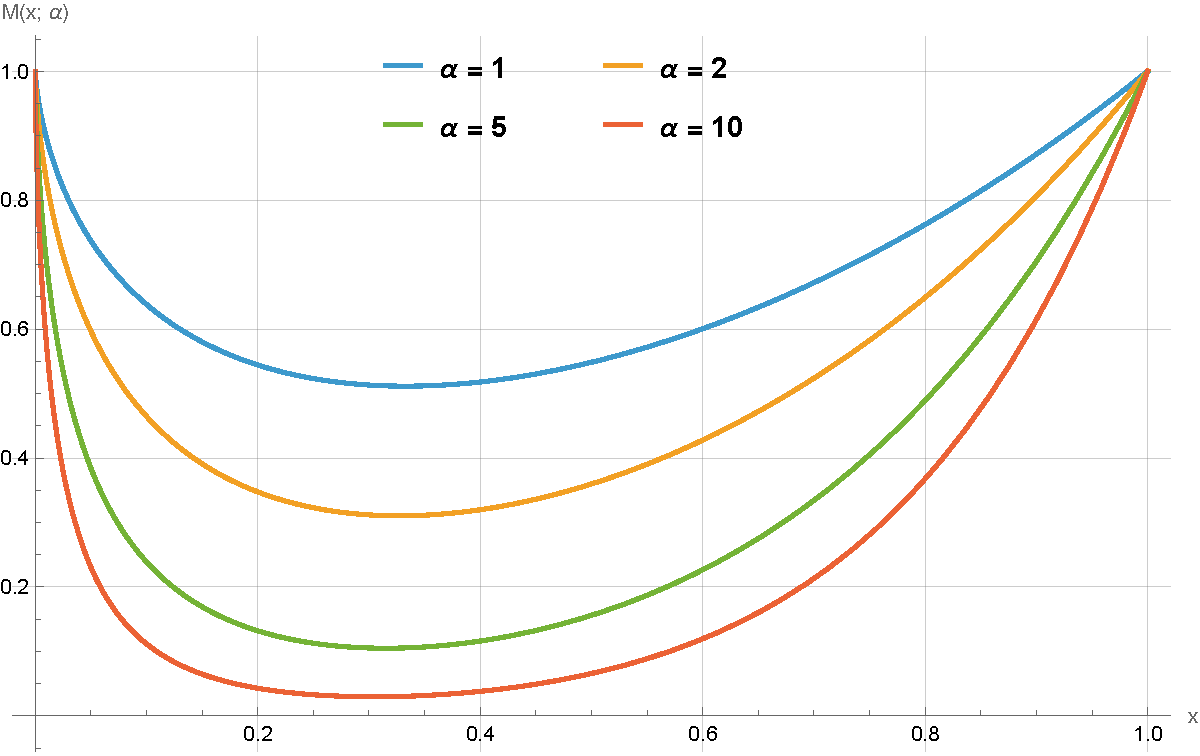
\includegraphics[width=0.5\linewidth]{img/validation/fgm.pdf}
    \caption{Visualisation de la \acl{FGM} $M(x;\alpha)$}\label{fig:FGMVisualisation}
\end{figure}
\FloatBarrier\paragraph{Analyse}\phantom{}\\
Il est important de souligner les points suivants:
\begin{itemize}
    \item Les conditions aux limites $M(0; \alpha) = M(c; \alpha) = 1$ sont respectées;
    \item Puisque $\alpha$ est par définition un paramètre positif (\ref{fgm}), la fonction est bien comprise dans l'intervalle $(0, 1)$, car elle correspond à l'exponentielle d'un nombre négatif; 
    \item Par ailleurs, et pour la même raison, lorsque $\alpha$ augmente, la fonction diminue.
\end{itemize}

L'expression obtenue pour la \acl{FGM} est ainsi validée. 


\subsection{Fonction Temps Moyen}

\paragraph{Visualisation}\phantom{}\\
Ensuite, il est nécessaire de valider le comportement de la fonction Temps Moyen $m(x)$ définie par (\ref{mean}), (\ref{sol_mean}) et (\ref{mean_constants}). La fonction est donc tracée pour différentes valeurs des paramètres $a,\;\forall\;a\in\{0.1,0.2,0.4\}$ et $\sigma,\;\forall\;\sigma\in\{1,\sqrt{2},2\}$.


\begin{figure}[htb]
    \centering
    \begin{subfigure}{0.45\linewidth}
        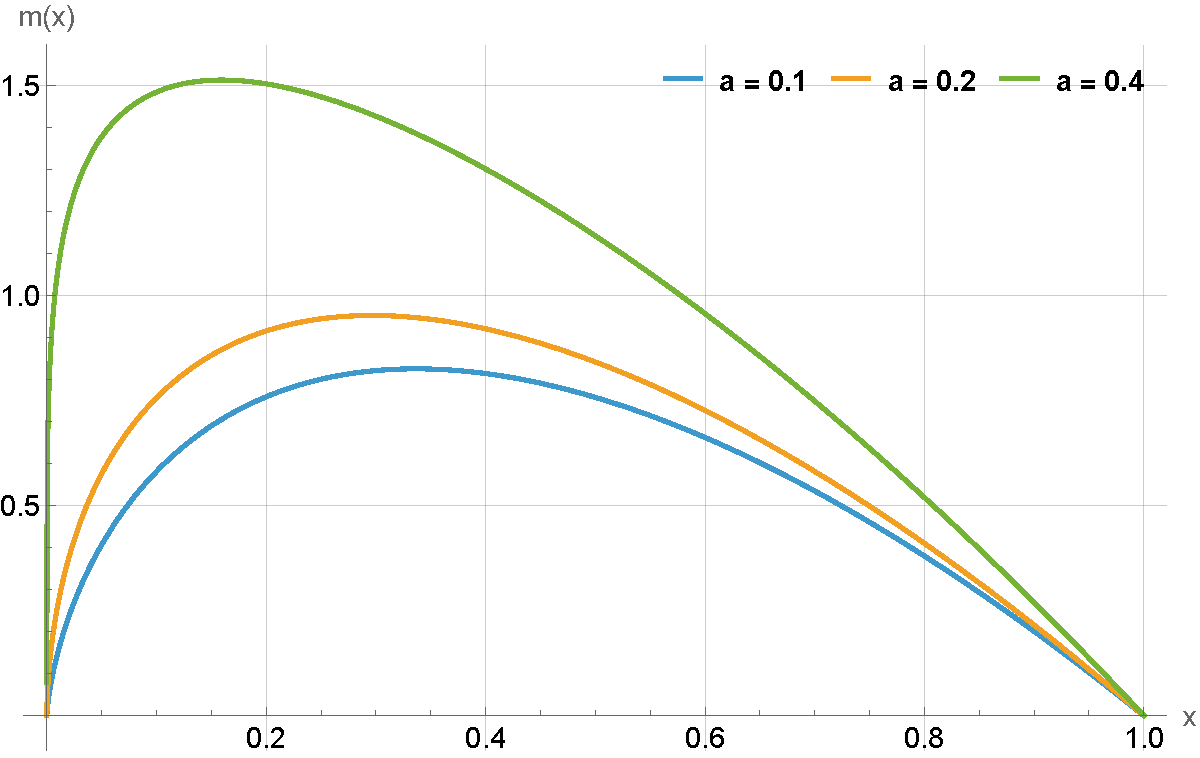
\includegraphics[width=\linewidth]{img/validation/Mean/mean_a.pdf}
        \caption{Sensibilité de la vitesse $a$}\label{fig:Mean_a_visualisation}
    \end{subfigure}
    \hfill
    \begin{subfigure}{0.45\linewidth}
        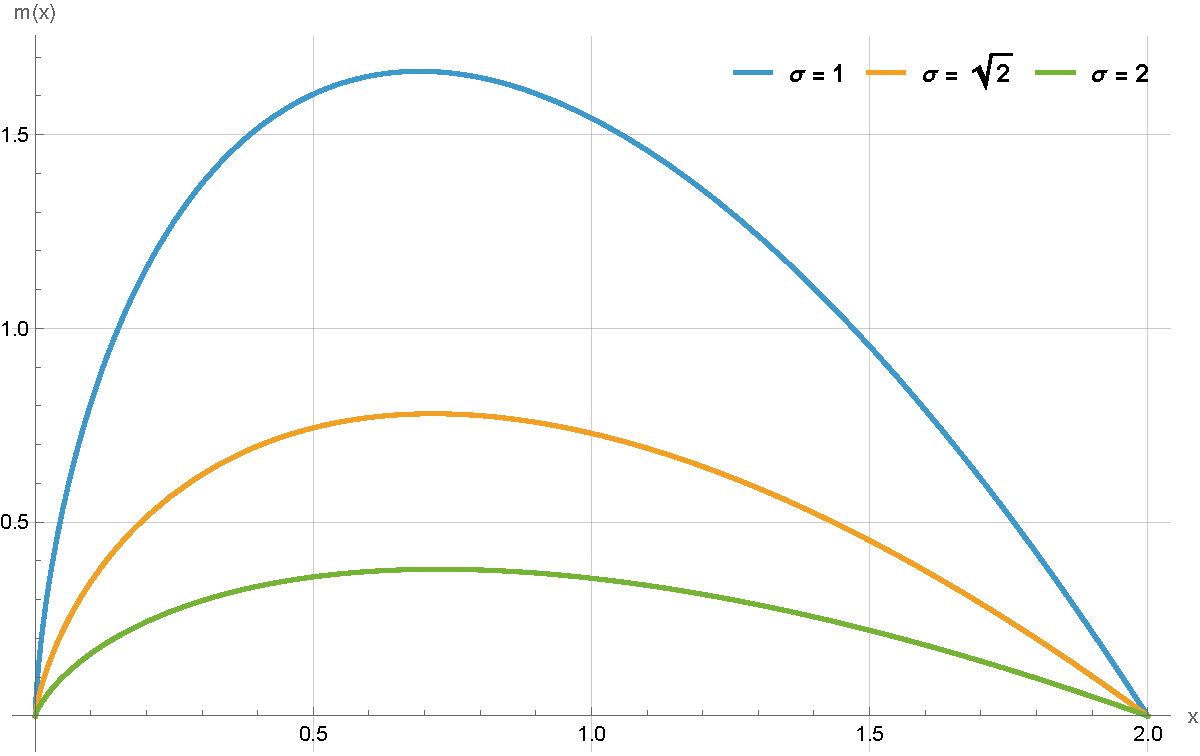
\includegraphics[width=\linewidth]{img/validation/Mean/mean_sigma.pdf}
        \caption{Sensibilité de la volatilité infinitésimale $\sigma$}\label{fig:Mean_sigma_visualisation}
    \end{subfigure}
    \caption{Visualisation de la fonction Temps Moyen $m(x)$}\label{fig:MeanVisualisation}
\end{figure}
\FloatBarrier\paragraph{Analyse}\phantom{}\\
Il est important de noter les points suivants concernant toutes les valeurs différentes des paramètres:
\begin{itemize}
    \item Les conditions aux limites $m(0)=m(c)=0$ sont respectées;
    \item Cette fonction représente un \textit{temps moyen de premier passage}, elle doit donc être positive pour toute valeur de $x$ dans $[0,c]$;
    \item Une augmentation de la vitesse de retour $a$ entraîne une hausse du temps moyen de sortie de l'intervalle. En effet, plus la force de rappel vers la moyenne est forte (i.e., $a$ élevé), plus une déviation significative et peu probable est nécessaire pour franchir les bornes de l'intervalle;
    \item À l'inverse, une augmentation de la volatilité infinitésimale $\sigma$ diminue le temps moyen de sortie. Cela s'explique naturellement: des fluctuations plus intenses accroissent la probabilité de quitter rapidement l'intervalle.
\end{itemize}

L'expression obtenue pour la fonction de temps moyen de premier passage est ainsi validée.

\subsection{Fonction Aire Moyenne}

\paragraph{Visualisation}\phantom{}\\
Par ailleurs, la même démarche de validation est effectuée pour la fonction Aire Moyenne $A(x)$ définie par (\ref{area}), (\ref{sol_area}) et (\ref{area_constants}).

\begin{figure}[htb]
    \centering
    \begin{subfigure}{0.45\linewidth}
        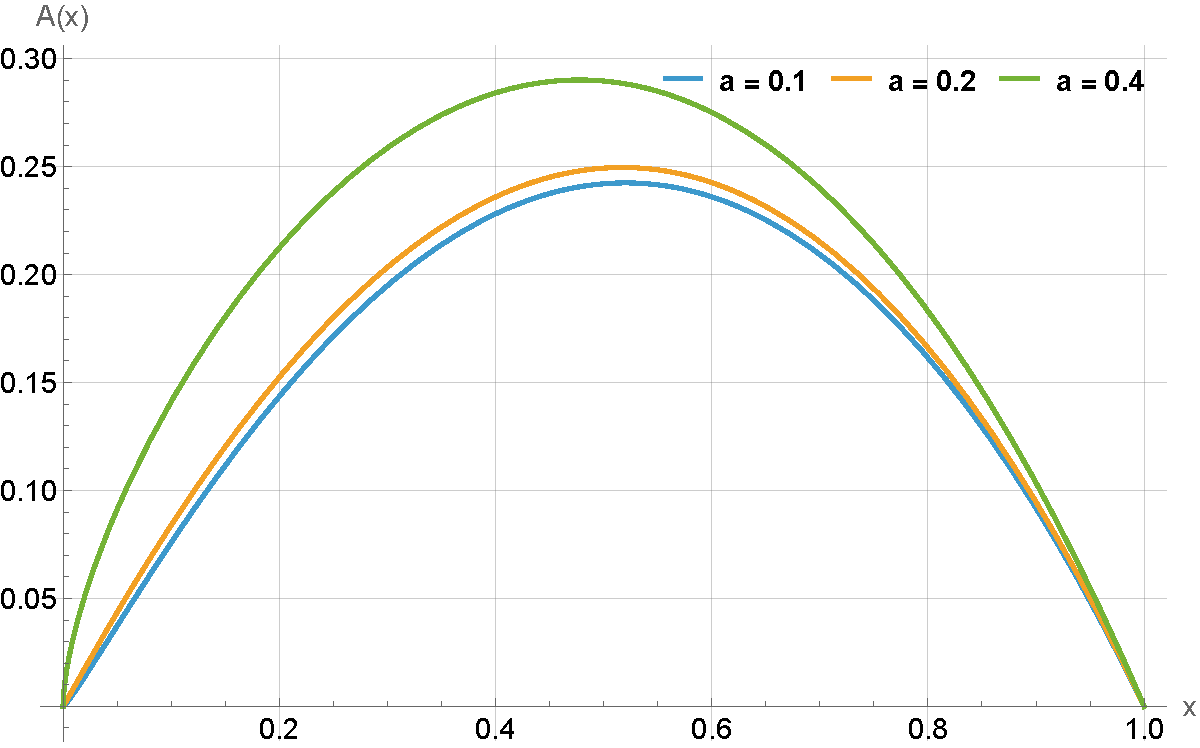
\includegraphics[width=\linewidth]{img/validation/Area/area_a.pdf}
        \caption{Sensibilité de la vitesse $a$}\label{fig:Area_a_visualisation}
    \end{subfigure}
    \hfill
    \begin{subfigure}{0.45\linewidth}
        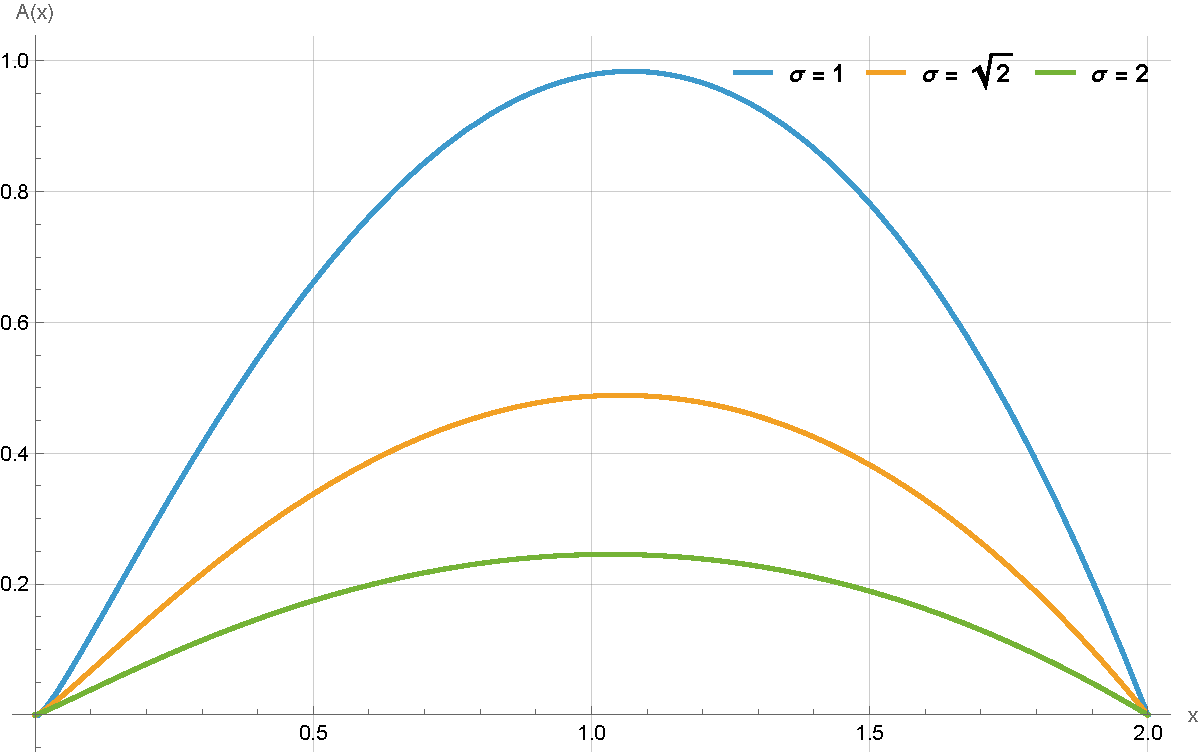
\includegraphics[width=\linewidth]{img/validation/Area/area_sigma.pdf}
        \caption{Sensibilité de la volatilité infinitésimale $\sigma$}\label{fig:Area_sigma_visualisation}
    \end{subfigure}
    \caption{Visualisation de la fonction Aire Moyenne $A(x)$}\label{fig:AreaVisualisation}
\end{figure}
\FloatBarrier\paragraph{Analyse}\phantom{}\\
Il convient de souligner les points suivants:
\begin{itemize}
    \item Les conditions aux limites $A(0)=A(c)=0$ sont respectées;
    \item Cette fonction représente une \textit{aire moyenne} sous un processus positif, elle doit donc être positive pour toute valeur de $x$ dans $[0,c]$;
    \item Une augmentation de la vitesse de retour $a$ entraîne une augmentation de l'aire moyenne sous le processus avant la sortie de l'intervalle. En effet, une force de rappel plus intense maintient le processus autour de sa moyenne plus longtemps, retardant la sortie et augmentant ainsi l'accumulation totale;
    \item À l'inverse, une augmentation de la volatilité infinitésimale $\sigma$ réduit l'aire moyenne. Des fluctuations plus fortes rendent les sorties plus précoces, limitant la durée pendant laquelle le processus peut contribuer à l'intégrale.
\end{itemize}

L'expression obtenue pour la fonction Aire Moyenne est ainsi validée.

\subsection{Commande Optimale Stochastique}

Enfin, il est nécessaire de valider les expressions obtenues dans le cadre des trois problèmes de commande optimale étudiés. Pour cela, il convient de tracer la fonction valeur $F(x)$ ainsi que le contrôle optimal $u^*(x)$, et s'il est possible, pour plusieurs valeurs des différents paramètres des coûts. Afin d'isoler l'influence d'un paramètre lors de l'analyse, les autres seront fixés à $1$.

\subsubsection{Problème linéarisable 1 \textemdash~P1}\phantom{}\\
Le problème (\ref{p1}) est considéré. D'un côté, les fonctions $r(x)$, $b(x)$ et $q(x)$ sont définies en (\ref{p1}). D'un autre côté, la fonction valeur $F(x)$ est définie par (\ref{sol_control_1},~\ref{control_constants}) et le contrôle optimal est défini par (\ref{optimal_control_1}). D'abord, tous les paramètres de coûts sont: $\rho=\beta=\kappa=1$.
\begin{figure}[htb]
    \centering
    \begin{subfigure}{0.45\linewidth}
        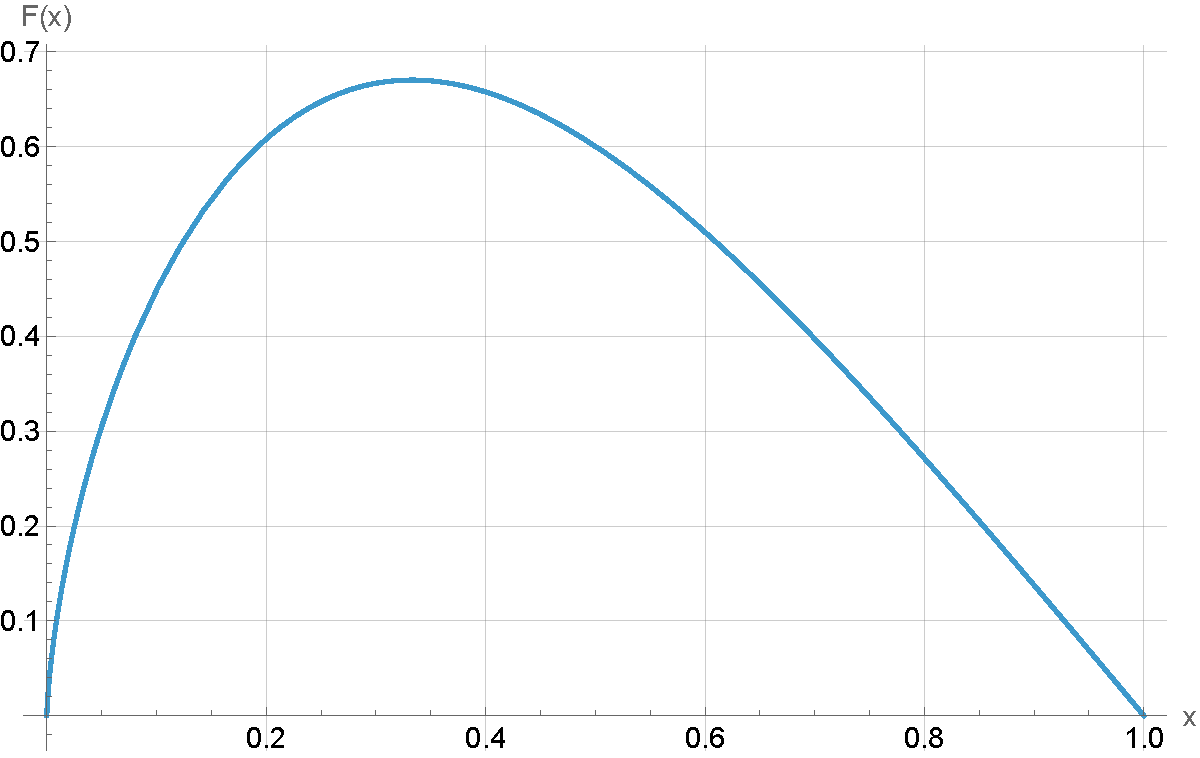
\includegraphics[width=\linewidth]{img/validation/P1/p1_value.pdf}
        \caption{P1 \textemdash~Fonction Valeur $F(x)$}\label{fig:ValueVisualisation1}
    \end{subfigure}
    \hfill
    \begin{subfigure}{0.45\linewidth}
        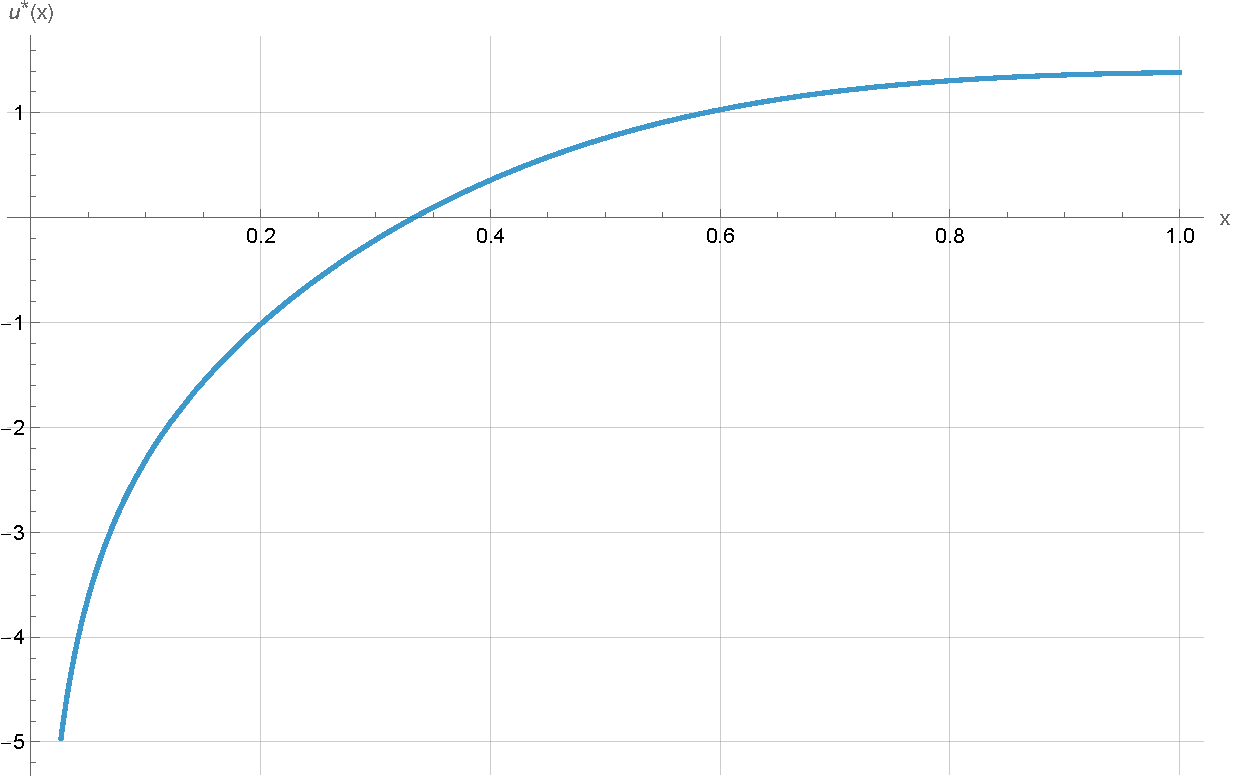
\includegraphics[width=\linewidth]{img/validation/P1/p1_control.pdf}
        \caption{P1 \textemdash~Contrôle Optimal $u^*(x)$}\label{fig:ControlVisualisation1}
    \end{subfigure}
    \caption{P1 \textemdash~Visualisation de la fonction valeur et du contrôle optimal}\label{fig:ValueControlComparison1}
\end{figure}\FloatBarrier De plus, il est intéressant d'analyser la sensibilité de ces fonctions par rapport à la variation des coûts. Les différentes valeurs des paramètres suivants sont évaluées:
\begin{itemize}
    \item Paramètre du coût immédiat $\rho,\;\forall\;\rho\in\{1,2,5,10\}$
    \item Paramètre du coût de contrôle $\beta,\;\forall\;\beta\in\{1,2,3,4\}$
    \item Paramètre du poids pénalisant l'intensité du contrôle $\kappa,\;\forall\;\kappa\in\{1,2,5,10\}$
\end{itemize}
\begin{figure}[htb]
    \centering
    \begin{subfigure}{0.45\linewidth}
        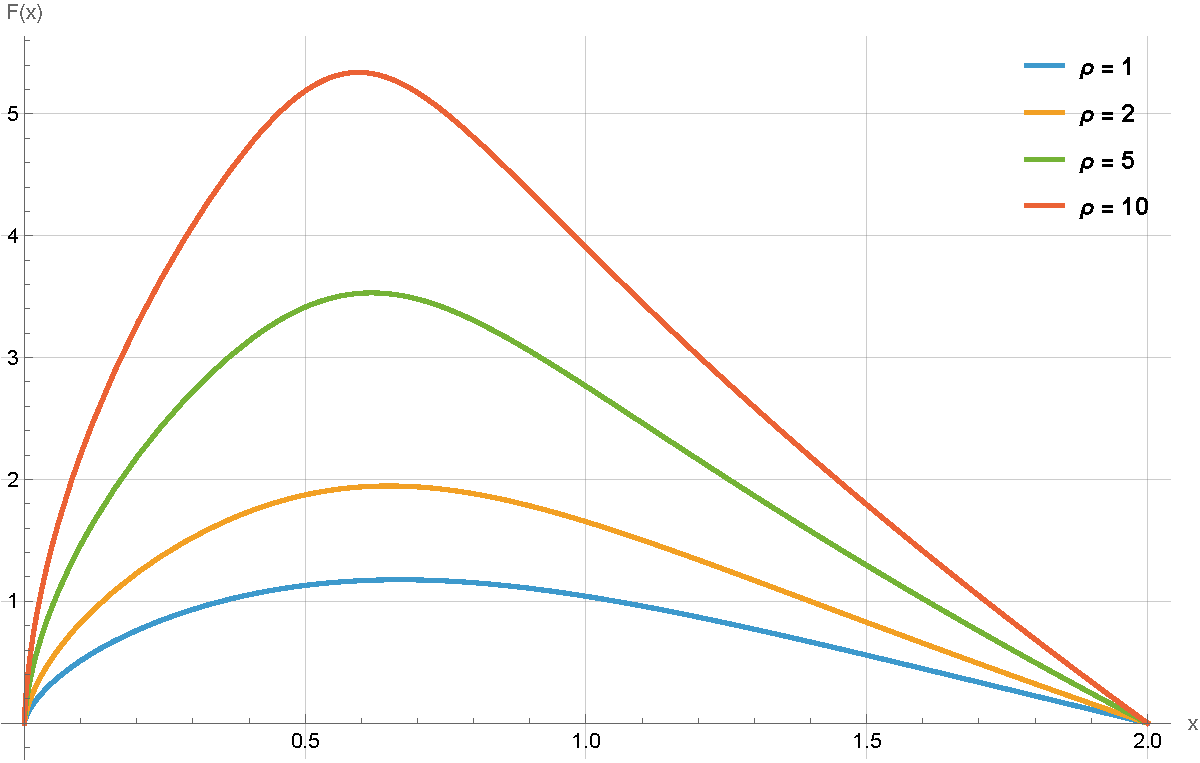
\includegraphics[width=\linewidth]{img/validation/P1/p1_R_value.pdf}
        \caption{P1 \textemdash~Fonction Valeur $F(x)$}\label{fig:RhoValueVisualisation1}
    \end{subfigure}
    \hfill
    \begin{subfigure}{0.45\linewidth}
        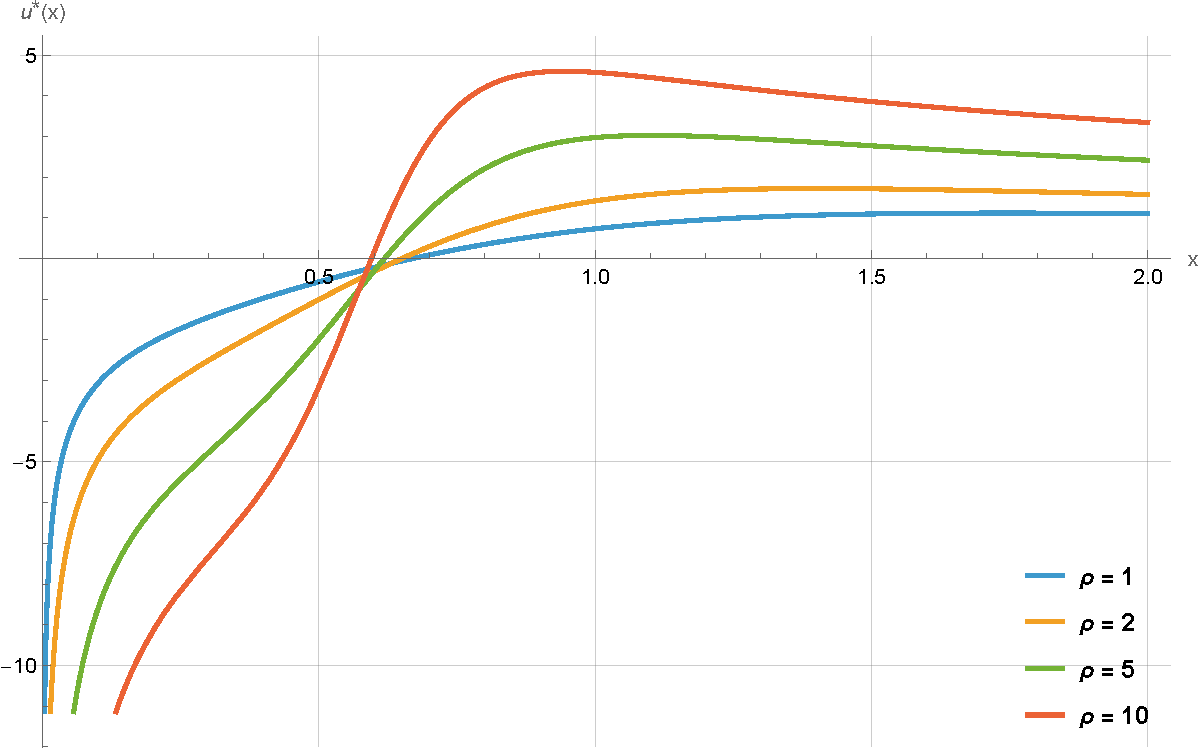
\includegraphics[width=\linewidth]{img/validation/P1/p1_R_control.pdf}
        \caption{P1 \textemdash~Contrôle Optimal $u^*(x)$}\label{fig:RhoControlVisualisation1}
    \end{subfigure}
    \caption{P1 \textemdash~Sensibilité du coût immédiat $r(x)=\rho$}\label{fig:RhoValueControlComparison1}
\end{figure}
\FloatBarrier\begin{figure}[htb]
    \centering
    \begin{subfigure}{0.45\linewidth}
        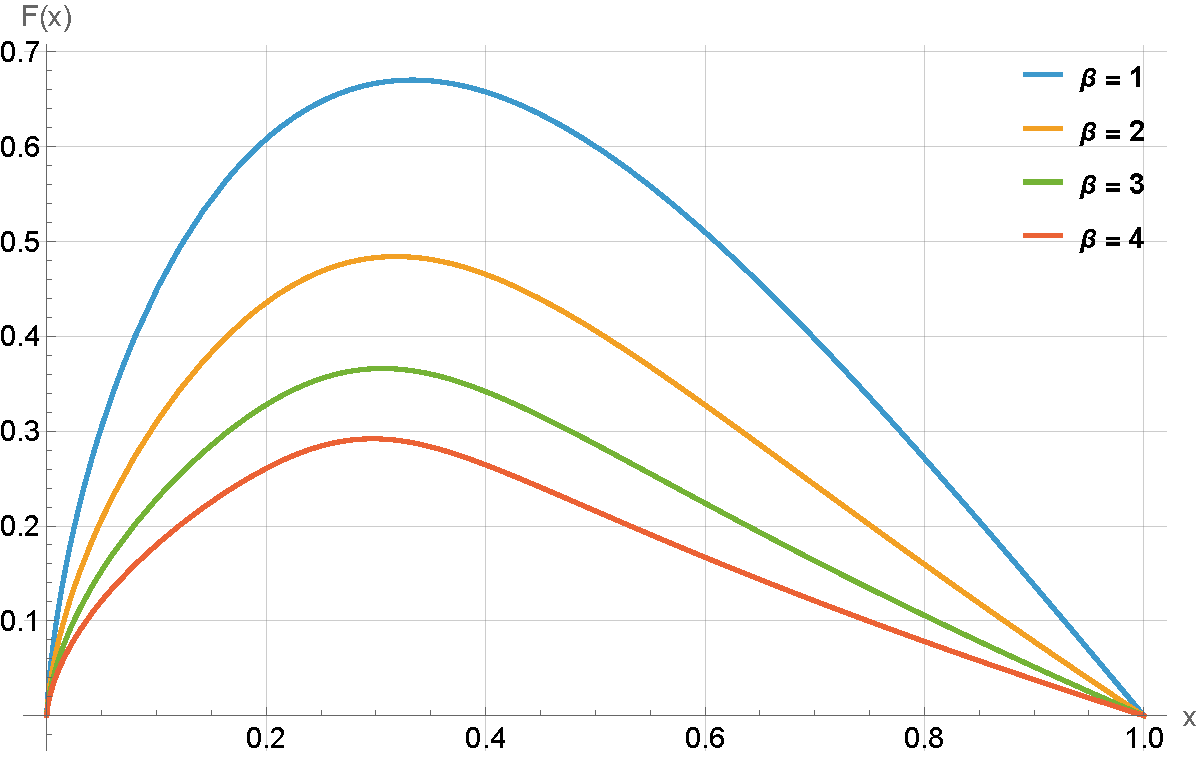
\includegraphics[width=\linewidth]{img/validation/P1/p1_B_value.pdf}
        \caption{P1 \textemdash~Fonction Valeur $F(x)$}\label{fig:BetaValueVisualisation1}
    \end{subfigure}
    \hfill
    \begin{subfigure}{0.45\linewidth}
        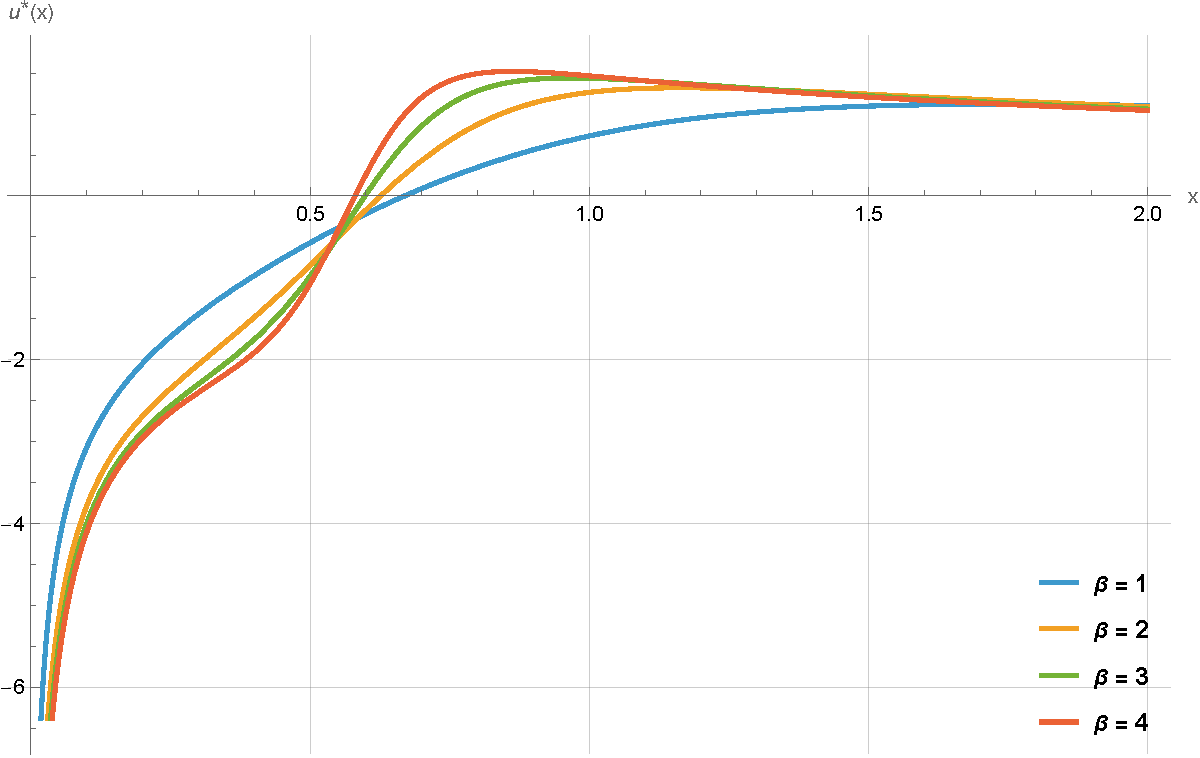
\includegraphics[width=\linewidth]{img/validation/P1/p1_B_control.pdf}
        \caption{P1 \textemdash~Contrôle Optimal $u^*(x)$}\label{fig:BetaControlVisualisation1}
    \end{subfigure}
    \caption{P1 \textemdash~Sensibilité du coût du contrôle $b(x)=\beta x$}\label{fig:BetaValueControlComparison}
\end{figure}
\FloatBarrier\begin{figure}[htb]
    \centering
    \begin{subfigure}{0.45\linewidth}
        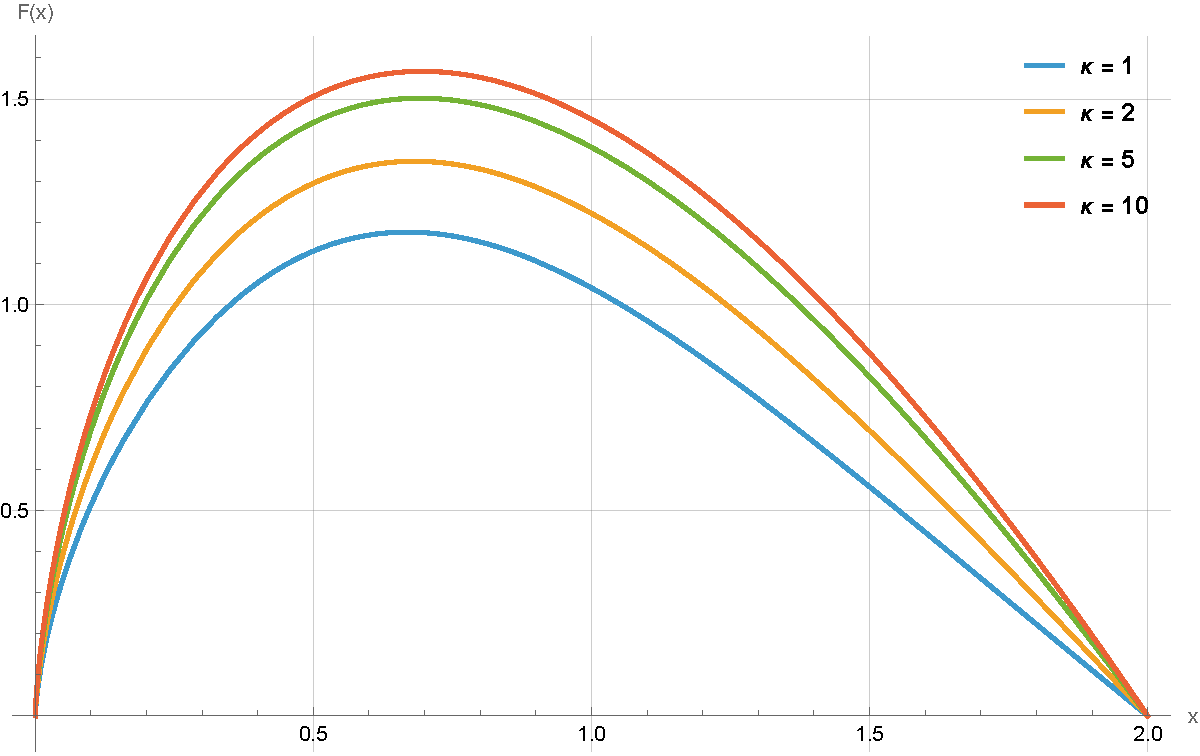
\includegraphics[width=\linewidth]{img/validation/P1/p1_K_value.pdf}
        \caption{P1 \textemdash~Fonction Valeur $F(x)$}\label{fig:KappaValueVisualisation1}
    \end{subfigure}
    \hfill
    \begin{subfigure}{0.45\linewidth}
        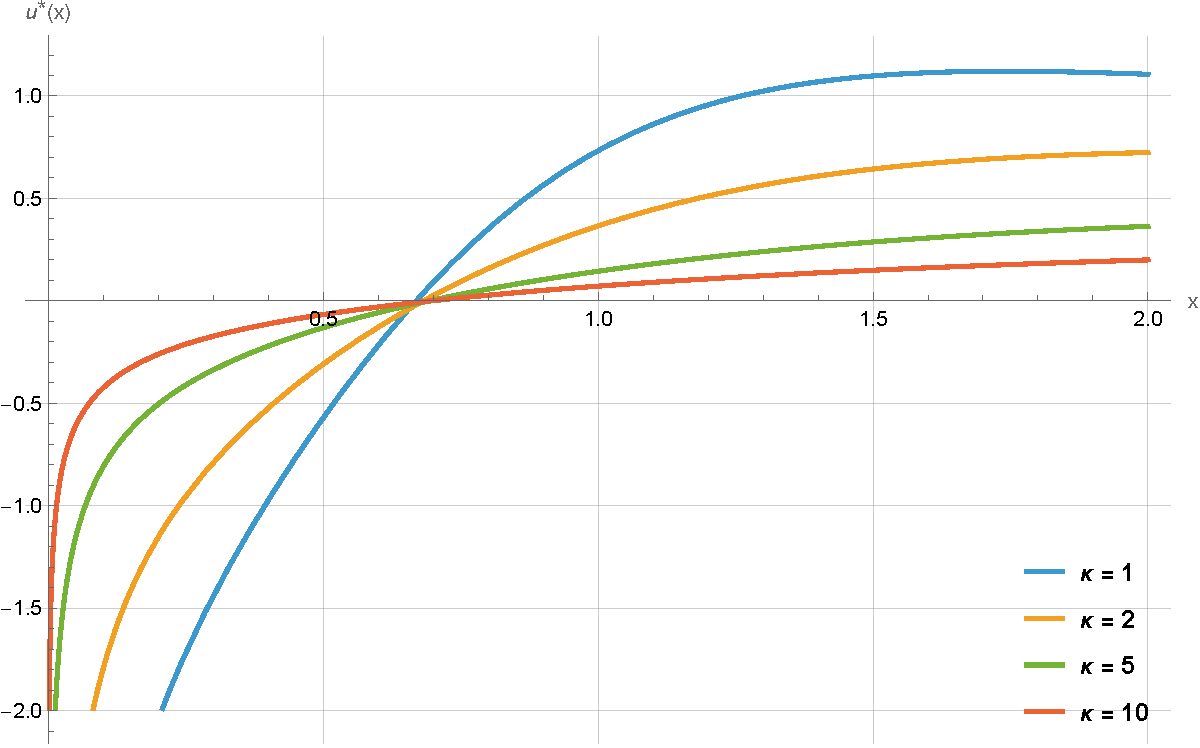
\includegraphics[width=\linewidth]{img/validation/P1/p1_K_control.pdf}
        \caption{P1 \textemdash~Contrôle Optimal $u^*(x)$}\label{fig:KappaControlVisualisation1}
    \end{subfigure}
    \caption{P1 \textemdash~Sensibilité de la pondération du contrôle $q(x)=\kappa x$}\label{fig:KappaValueControlComparison1}
\end{figure}
\FloatBarrier Une simulation d'une trajectoire contrôlée et d'une trajectoire non contrôlée est effectuée en utilisant un même tirage aléatoire, afin de permettre une comparaison pertinente entre les deux dynamiques. Les paramètres du processus \acs{CIR} sont ceux introduits en début de section, avec $\rho = \beta = \kappa = 1$.
\begin{figure}[htb]
    \centering
    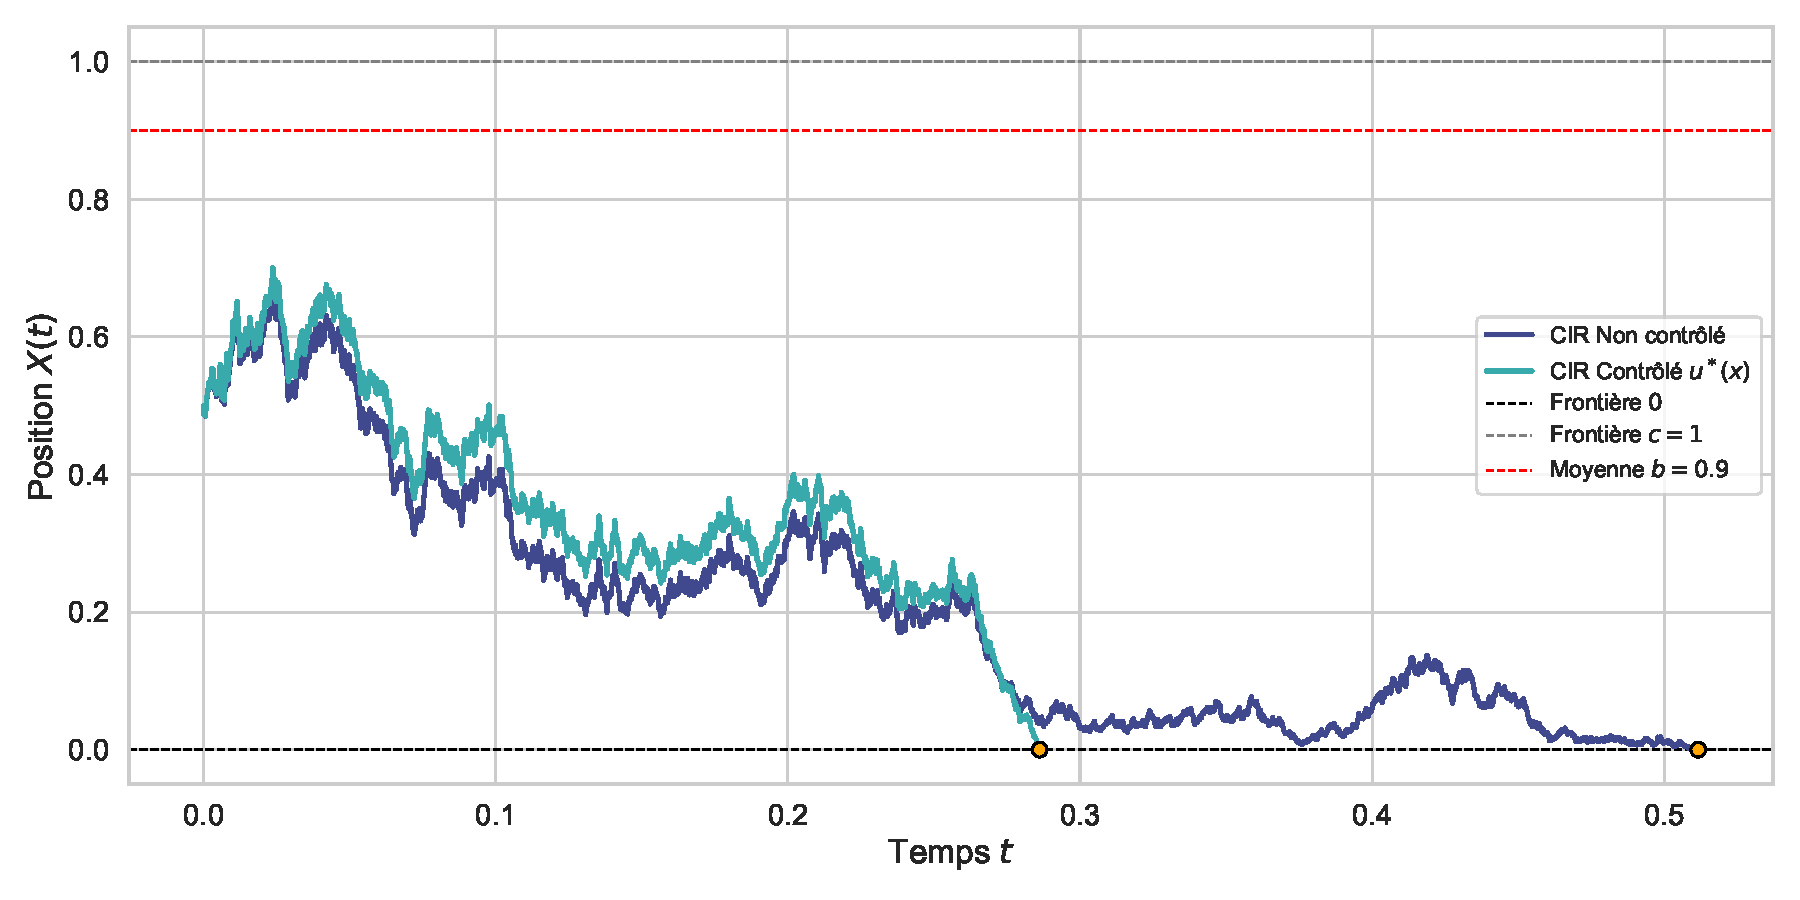
\includegraphics[width=0.9\linewidth]{img/validation/P1/p1_control_simulation.pdf}
    \caption{P1 \textemdash~Visualisation de l'effet de la commande optimale}
\end{figure}
\FloatBarrier\subsubsection{Problème linéarisable 2 \textemdash~P2}\phantom{}\\
Les résultats du problème (\ref{p2}) sont analysés. D'un côté, les fonctions $r(x)$, $b(x)$ et $q(x)$ sont définies en (\ref{p2}). D'un autre côté, la fonction valeur $F(x)$ est définie par (\ref{sol_control_2},~\ref{control_constants}) et le contrôle optimal est défini par (\ref{optimal_control_2}). Dans un premier temps, les coûts sont fixés: $\rho=\beta=\kappa=1$.
\begin{figure}[htb]
    \centering
    \begin{subfigure}{0.45\linewidth}
        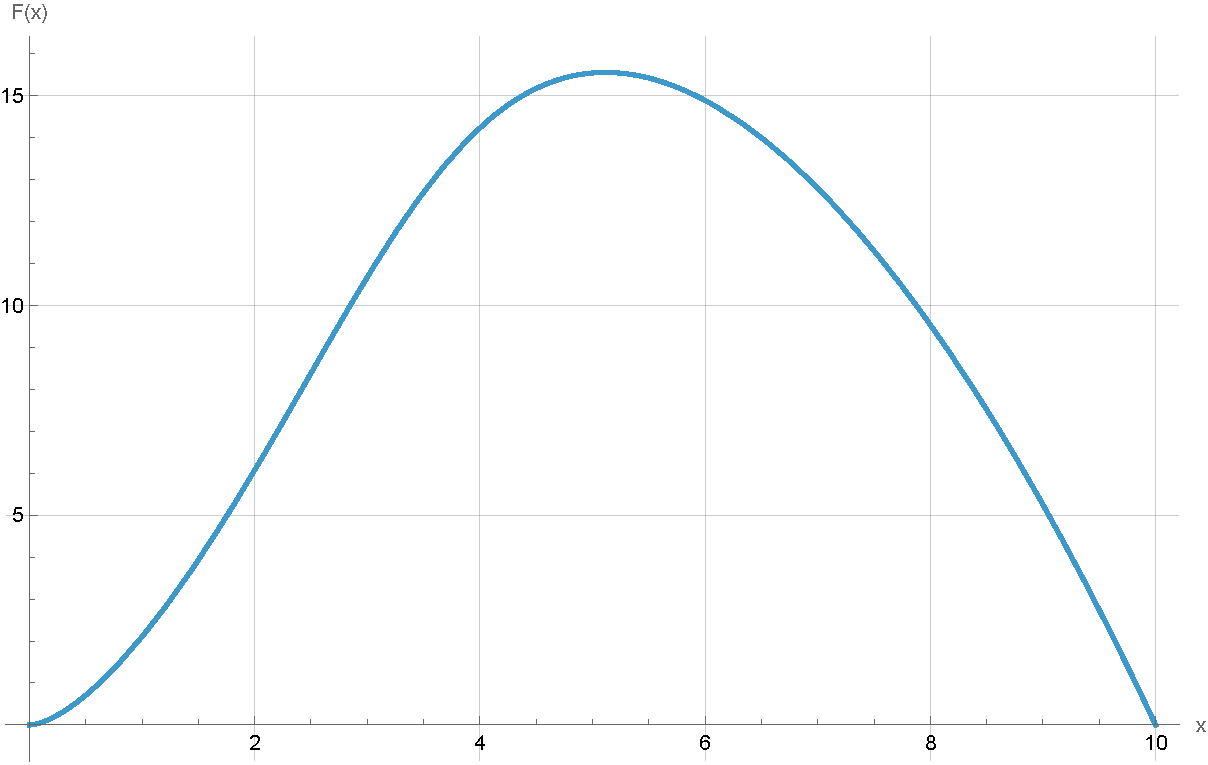
\includegraphics[width=\linewidth]{img/validation/P2/p2_value.pdf}
        \caption{P2 \textemdash~Fonction Valeur $F(x)$}\label{fig:ValueVisualisation2}
    \end{subfigure}
    \hfill
    \begin{subfigure}{0.45\linewidth}
        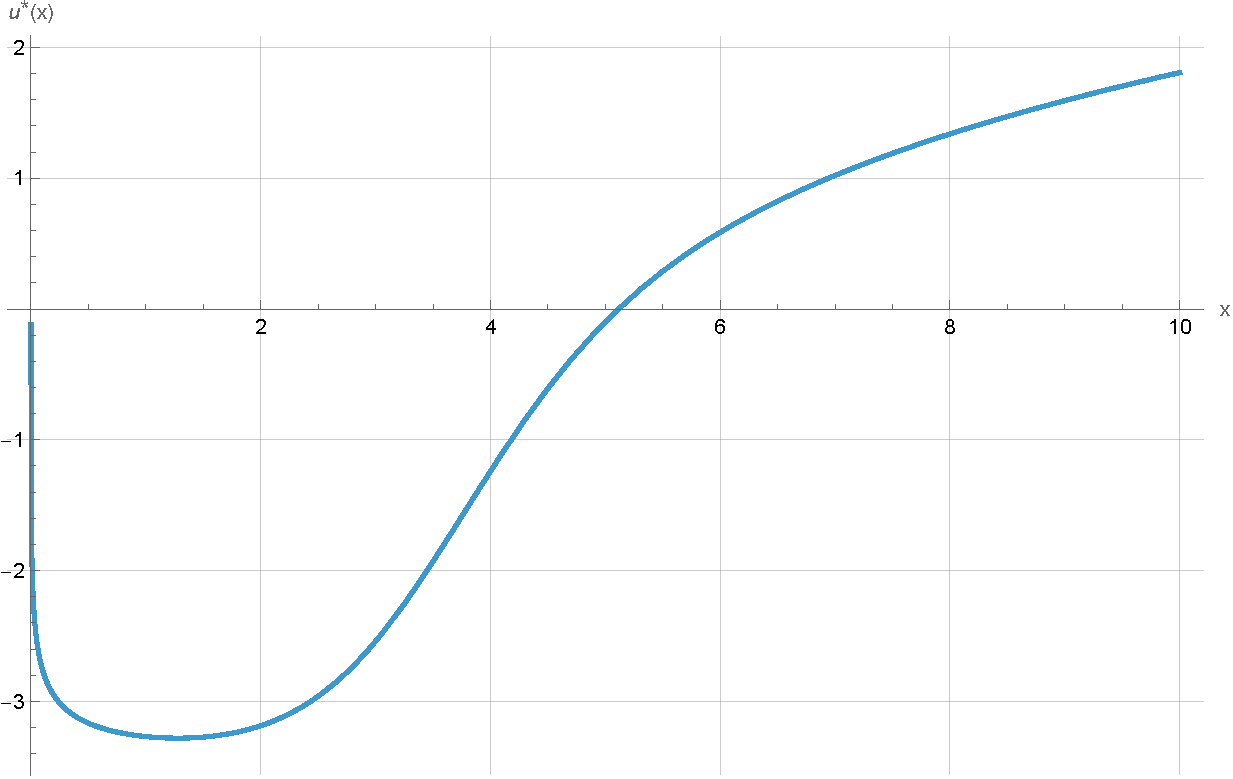
\includegraphics[width=\linewidth]{img/validation/P2/p2_control.pdf}
        \caption{P2 \textemdash~Contrôle Optimal $u^*(x)$}\label{fig:ControlVisualisation2}
    \end{subfigure}
    \caption{P2 \textemdash~Visualisation de la fonction valeur et du contrôle optimal}\label{fig:ValueControlComparison2}
\end{figure}\FloatBarrier Dans un second temps, et comme ce qui précède, la sensibilité des coûts est analysée, en fonction des mêmes valeurs paramètres $\rho$, $\beta$ et $\kappa$.
\begin{figure}[htb]
    \centering
    \begin{subfigure}{0.45\linewidth}
        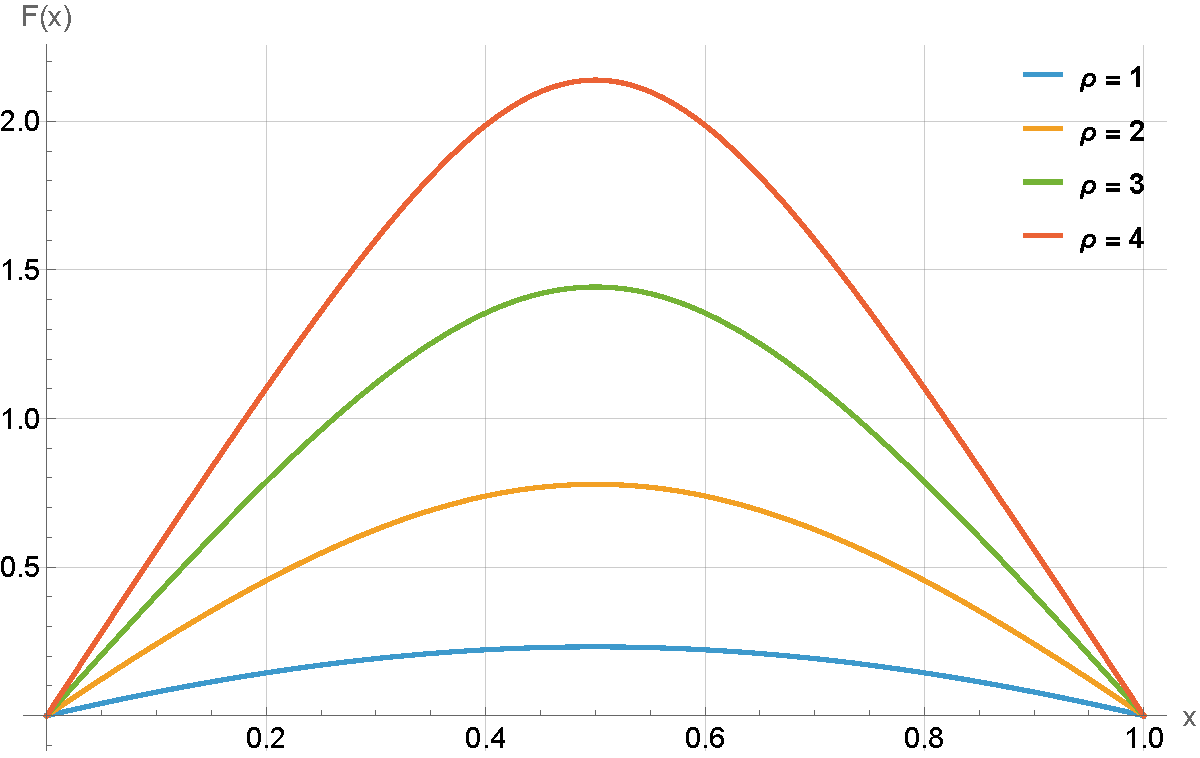
\includegraphics[width=\linewidth]{img/validation/P2/p2_R_value.pdf}
        \caption{P2 \textemdash~Fonction Valeur $F(x)$}\label{fig:RhoValueVisualisation2}
    \end{subfigure}
    \hfill
    \begin{subfigure}{0.45\linewidth}
        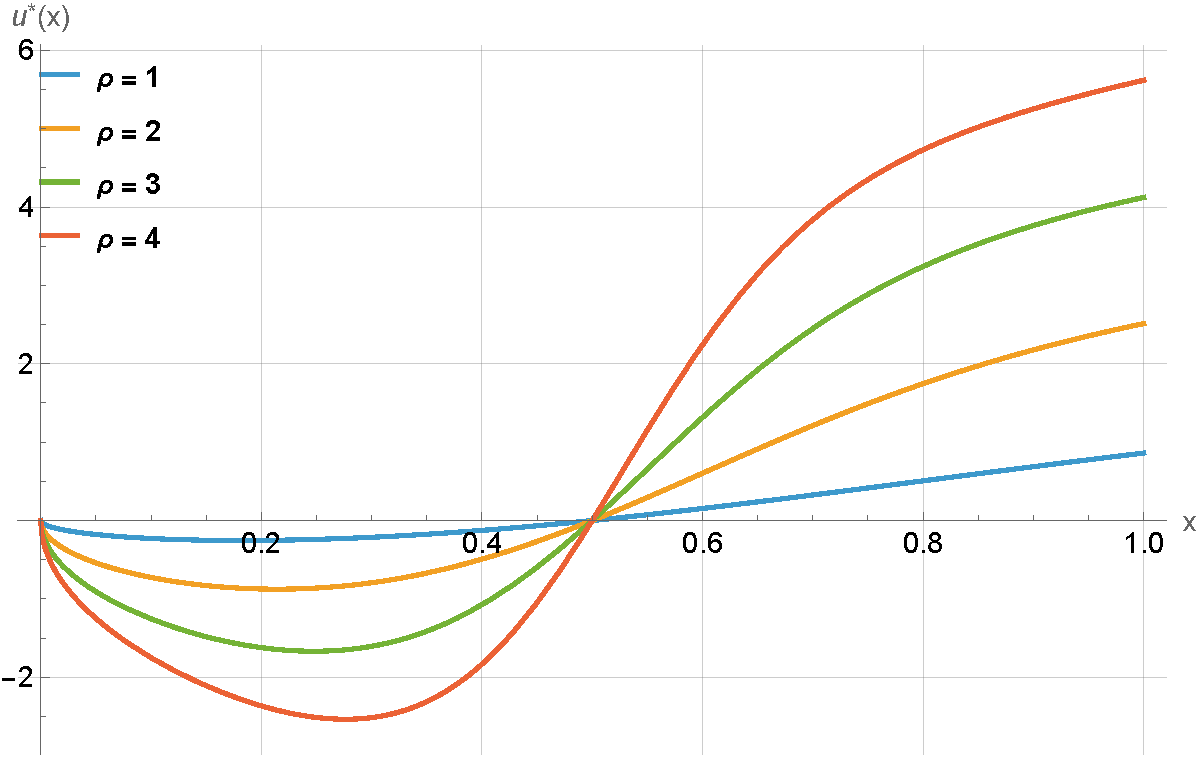
\includegraphics[width=\linewidth]{img/validation/P2/p2_R_control.pdf}
        \caption{P2 \textemdash~Contrôle Optimal $u^*(x)$}\label{fig:RhoControlVisualisation2}
    \end{subfigure}
    \caption{P2 \textemdash~Sensibilité du coût immédiat $r(x)=\rho x$}\label{fig:RhoValueControlComparison2}
\end{figure}
\FloatBarrier\begin{figure}[htb]
    \centering
    \begin{subfigure}{0.45\linewidth}
        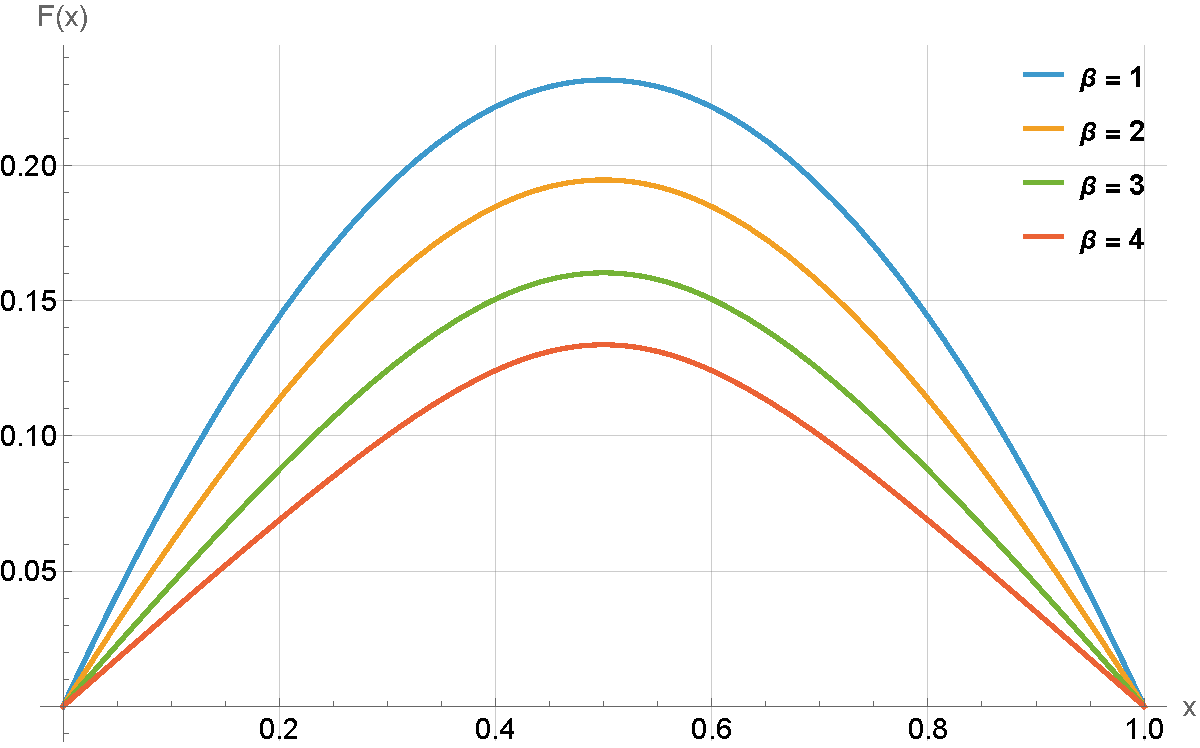
\includegraphics[width=\linewidth]{img/validation/P2/p2_B_value.pdf}
        \caption{P2 \textemdash~Fonction Valeur $F(x)$}\label{fig:BetaValueVisualisation2}
    \end{subfigure}
    \hfill
    \begin{subfigure}{0.45\linewidth}
        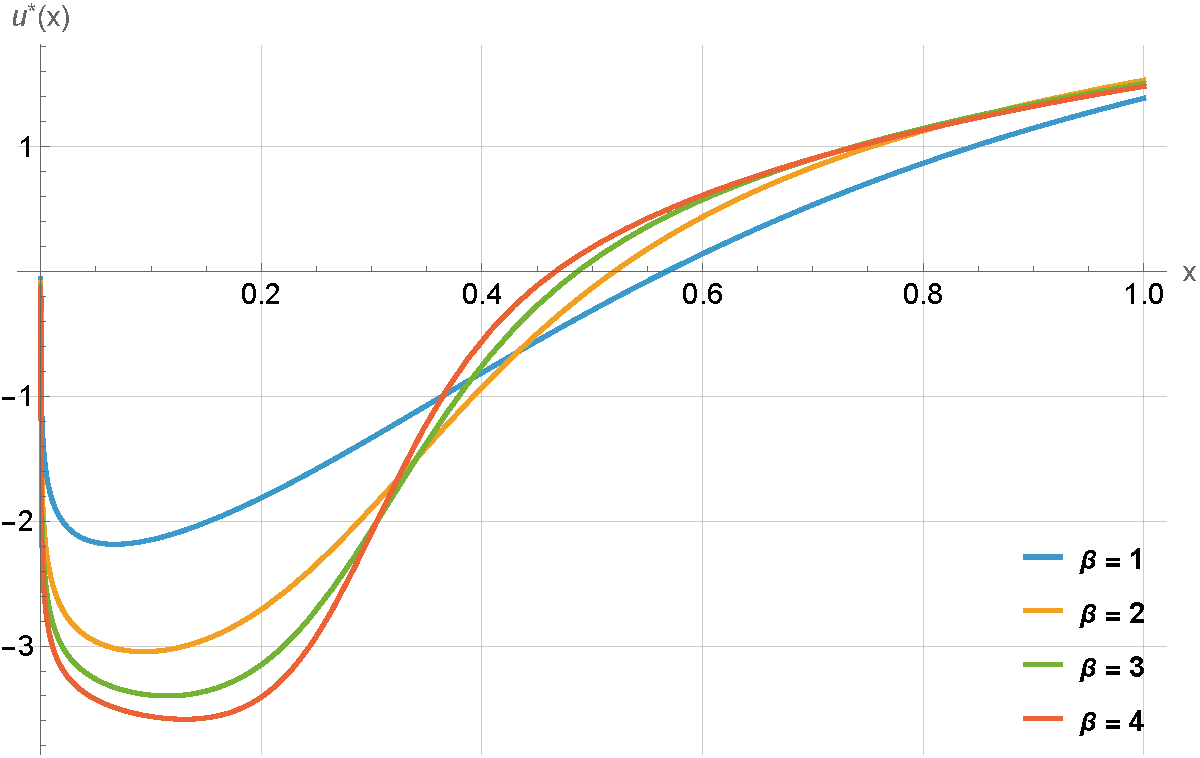
\includegraphics[width=\linewidth]{img/validation/P2/p2_B_control.pdf}
        \caption{P2 \textemdash~Contrôle Optimal $u^*(x)$}\label{fig:BetaControlVisualisation2}
    \end{subfigure}
    \caption{P2 \textemdash~Sensibilité du coût du contrôle $b(x)=\beta \sqrt{x}$}\label{fig:BetaValueControlComparison1}
\end{figure}
\FloatBarrier\begin{figure}[htb]
    \centering
    \begin{subfigure}{0.45\linewidth}
        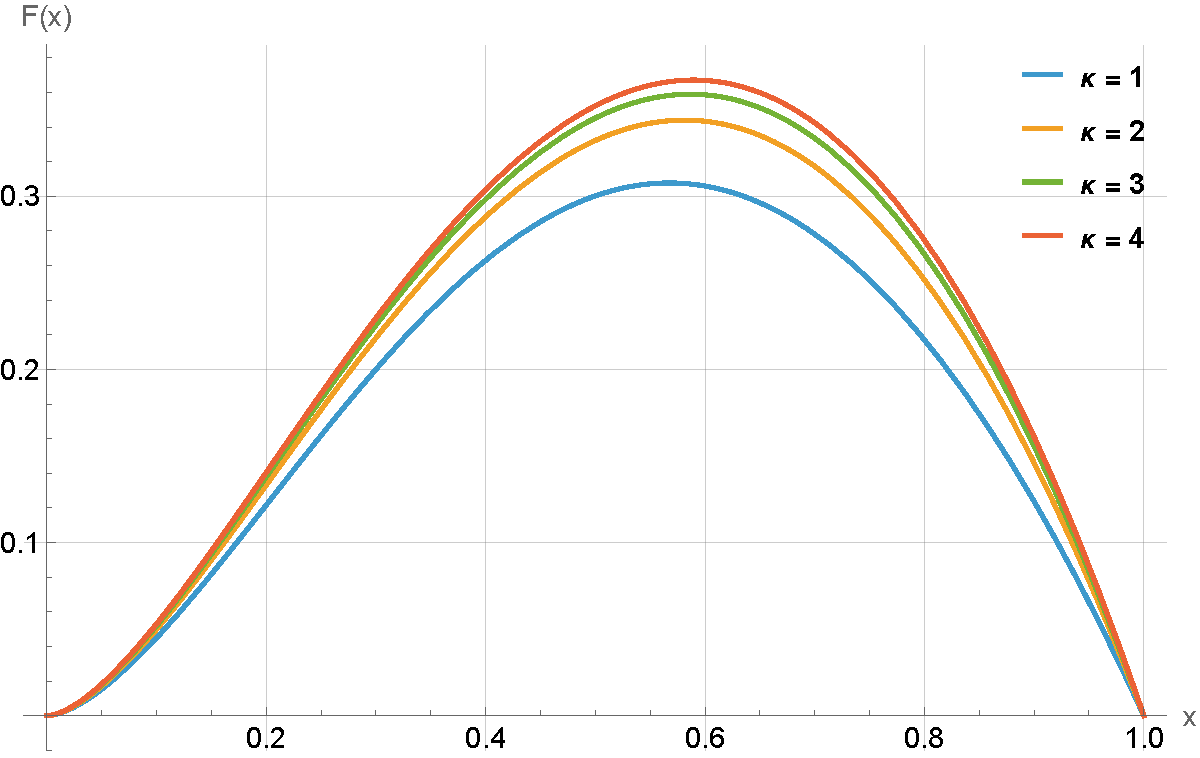
\includegraphics[width=\linewidth]{img/validation/P2/p2_K_value.pdf}
        \caption{P2 \textemdash~Fonction Valeur $F(x)$}\label{fig:KappaValueVisualisation2}
    \end{subfigure}
    \hfill
    \begin{subfigure}{0.45\linewidth}
        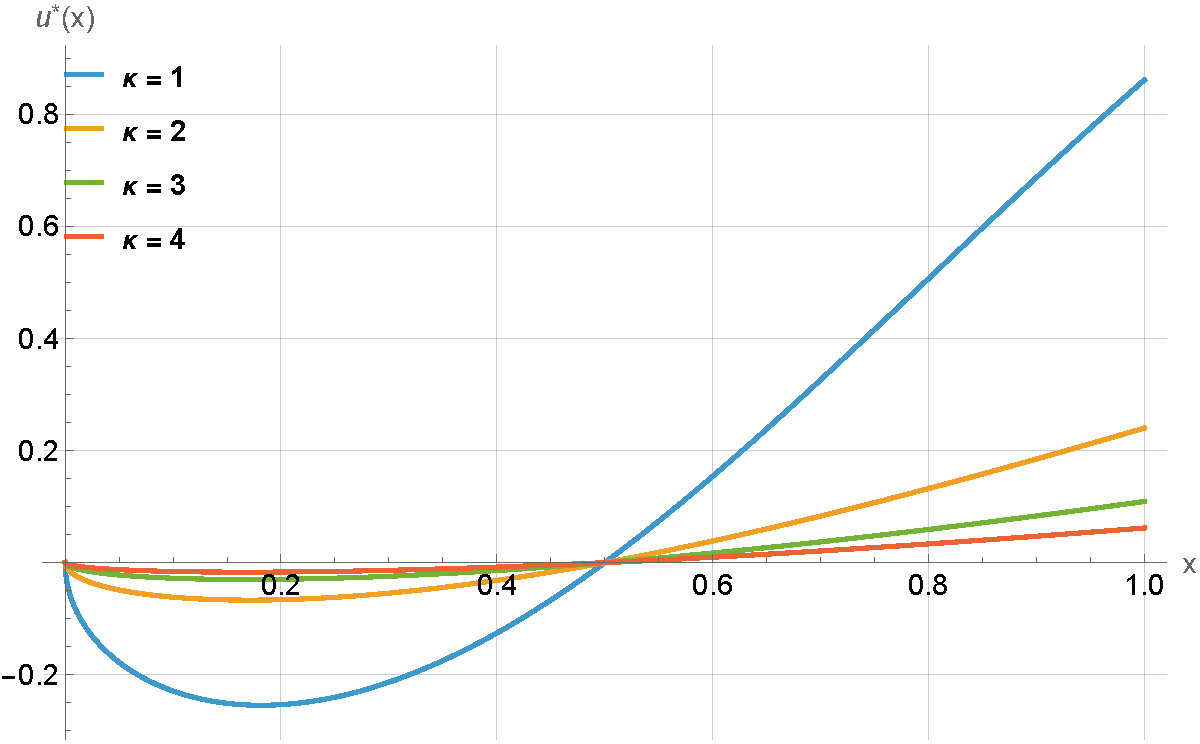
\includegraphics[width=\linewidth]{img/validation/P2/p2_K_control.pdf}
        \caption{P2 \textemdash~Contrôle Optimal $u^*(x)$}\label{fig:KappaControlVisualisation2}
    \end{subfigure}
    \caption{P2 \textemdash~Sensibilité de la pondération du contrôle $q(x)=\kappa x$}\label{fig:KappaValueControlComparison2}
\end{figure}
\FloatBarrier Comme précédemment, une trajectoire contrôlée est comparée à une trajectoire non contrôlée à partir d'un même tirage aléatoire. Les paramètres utilisés sont identiques à ceux de la dernière simulation.
\begin{figure}[htb]
    \centering
    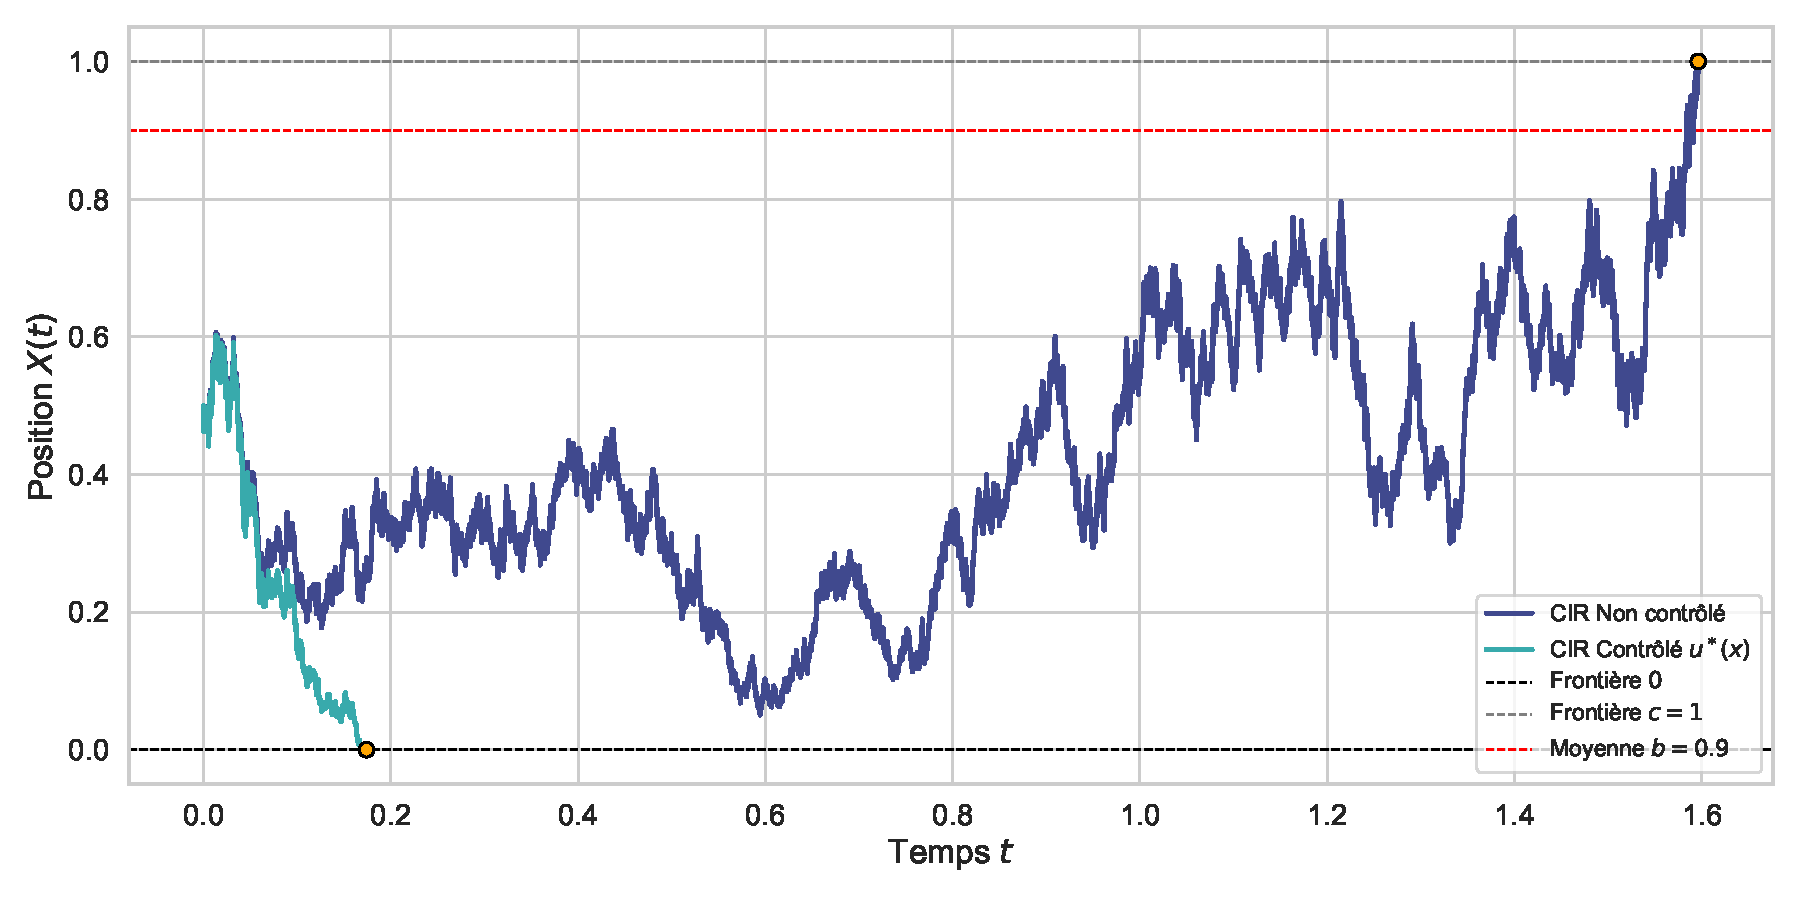
\includegraphics[width=0.9\linewidth]{img/validation/P2/p2_control_simulation.pdf}
    \caption{P2 \textemdash~Visualisation de l'effet de la commande optimale}
\end{figure}
\subsubsection{Problème non linéarisable \textemdash~P3}\phantom{}\\
Le problème (\ref{p3}) est porté à l'étude. L'expression de la fonction valeur (\ref{sol_control_3}) ainsi que la commande optimale (\ref{optimal_control_3}) sont tracés.
\begin{figure}[htb]
    \centering
    \begin{subfigure}{0.45\linewidth}
        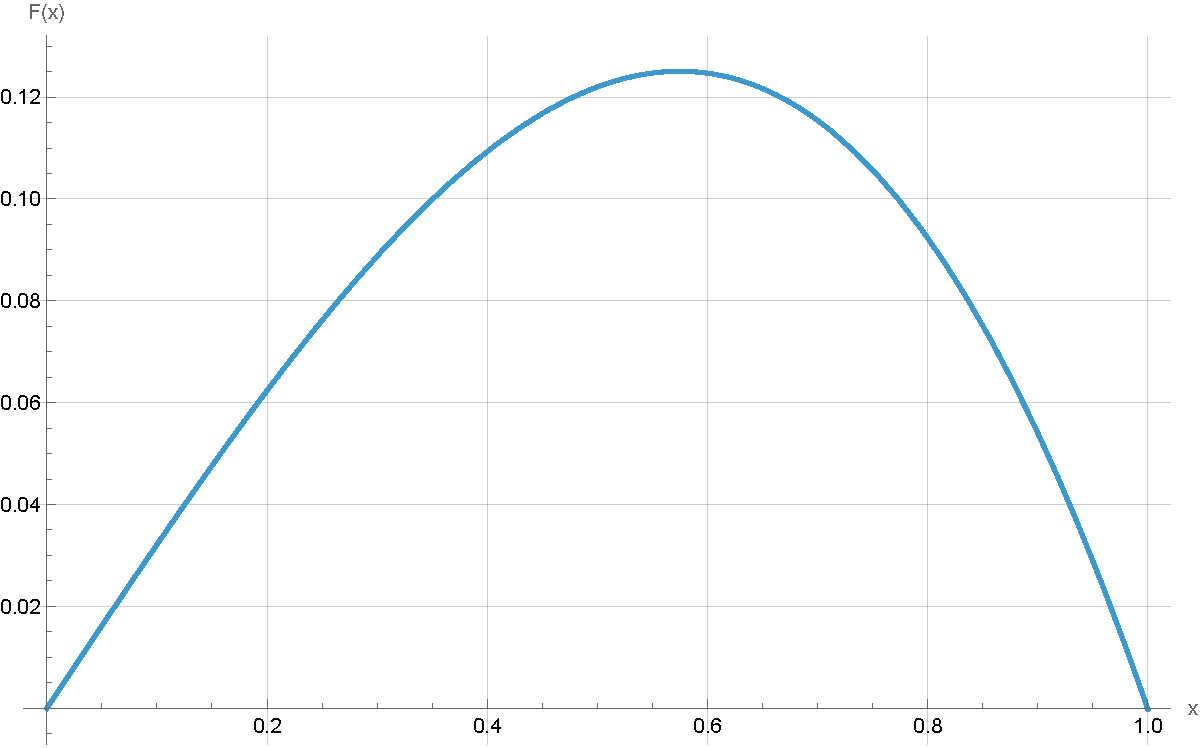
\includegraphics[width=\linewidth]{img/validation/P3/p3_value.pdf}
        \caption{P3 \textemdash~Fonction Valeur $F(x)$}\label{fig:ValueVisualisation3}
    \end{subfigure}
    \hfill
    \begin{subfigure}{0.45\linewidth}
        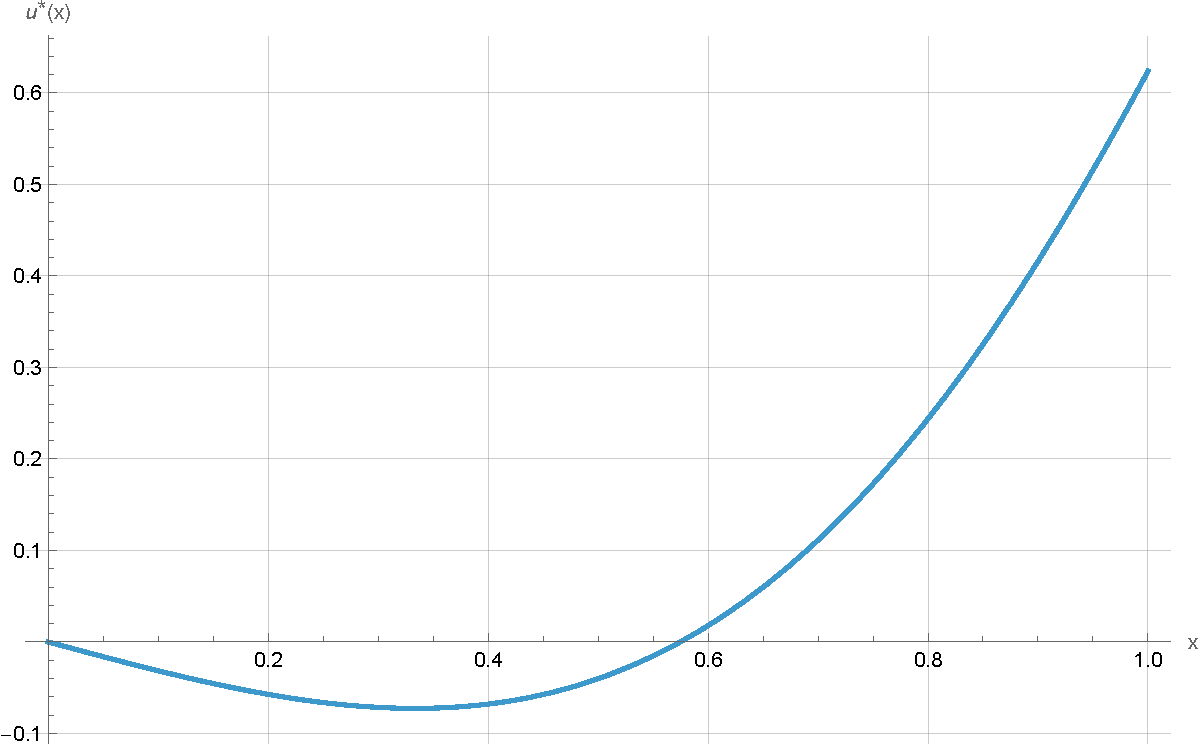
\includegraphics[width=\linewidth]{img/validation/P3/p3_control.pdf}
        \caption{P3 \textemdash~Contrôle Optimal $u^*(x)$}\label{fig:ControlVisualisation3}
    \end{subfigure}
    \caption{P3 \textemdash~Visualisation de la fonction valeur et du contrôle optimal}\label{fig:ValueControlComparison3}
\end{figure}
\FloatBarrier Toujours dans la même optique de visualisation de l'effet du contrôle, une simulation est effectuée. 
\begin{figure}[htb]
    \centering
    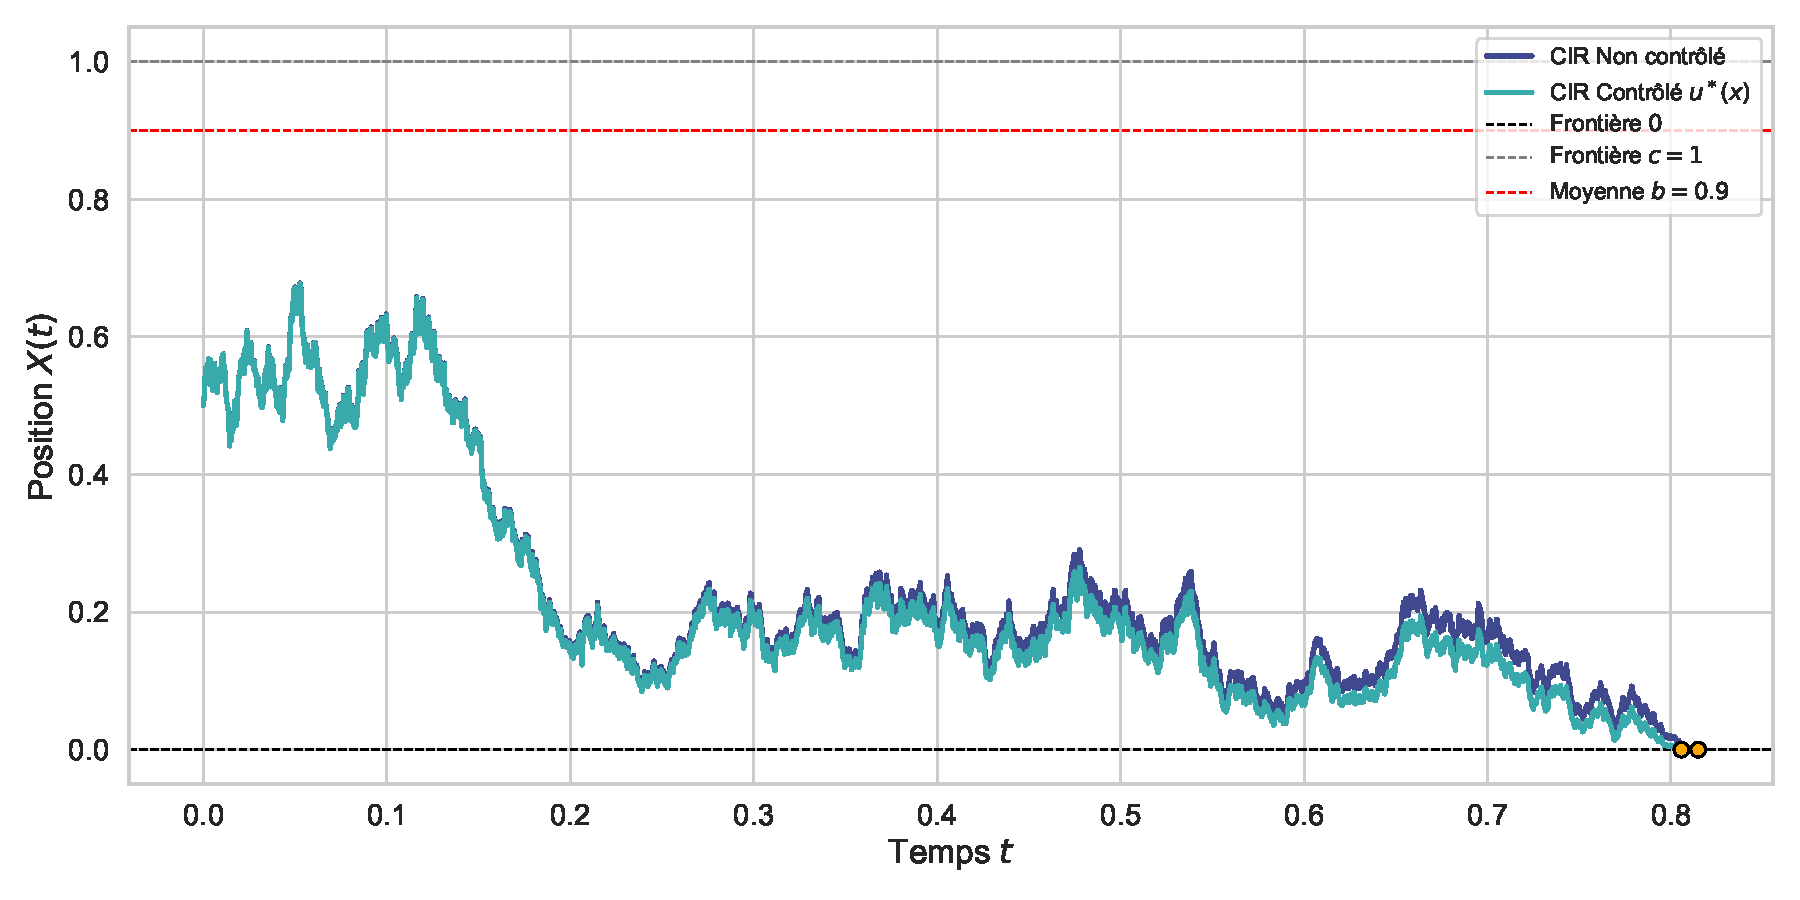
\includegraphics[width=0.9\linewidth]{img/validation/P3/p3_control_simulation.pdf}
    \caption{P3 \textemdash~Visualisation de l'effet de la commande optimale}\label{fig:Simulation3}
\end{figure}
\paragraph{Analyse}\phantom{}\\
Il est important de souligner que, dans les trois problèmes étudiés et pour les différentes valeurs des paramètres considérés:
\begin{itemize}
    \item Les conditions aux limites $F(0)=F(c)=0$ sont toujours respectées;
    \item La fonction valeur est toujours positive, le coût encouru étant nécessairement positif;
    \item Le contrôle optimal est généralement négatif sur \( x \in \left(0, \frac{c}{2}\right) \), l'optimiseur cherchant à diriger rapidement le processus vers la frontière \( 0 \), plus proche. Inversement, pour \( x \in \left(\frac{c}{2}, c\right) \), le contrôle devient positif afin d'accélérer l'atteinte de la frontière supérieure \( c \);
    \item Une augmentation du coût immédiat $\rho$, induisant une hausse du coût encouru, entraîne un renforcement du contrôle optimal ($|u^*(x)|$ augmente), traduisant ainsi une volonté accrue de quitter l'intervalle aussi rapidement que possible;
    \item Une hausse du coût du contrôle $\beta$ incite à intensifier le contrôle optimal afin de quitter l'intervalle plus rapidement. Cette stratégie réduit la durée d'exposition au coût instantané, ce qui compense partiellement le surcoût du contrôle et diminue le coût total encouru $F(x)$;
    \item Une augmentation du poids pénalisant le contrôle $\kappa$, induisant une hausse du coût encouru, entraîne une relaxation du contrôle optimal. En effet, plus le poids du contrôle est élevé, moins il est intéressant d'appliquer un contrôle fort;
    \item Les simulations mettent en évidence l'effet du contrôle optimal, qui accélère la sortie du processus par rapport au cas non contrôlé. Pour valider cette observation, 1000 trajectoires sont simulées pour chaque problème, et la durée moyenne jusqu'à la sortie est comparée. Un facteur d'accélération est ensuite estimé:
    \begin{table}[htb]
        \centering
        \caption{Comparaison des accélérations moyennes du temps de sortie}\label{tab:acceleration_results}
        \renewcommand{\arraystretch}{1.1}
        \begin{tabular}{||c|c||}
        \hline
        Problème de Commande & Accélération Moyenne \\\hline\hline
        P1 & 2.660552 \\
        P2 & 2.690582 \\
        P3 & 1.065163 \\\hline
        \end{tabular}
    \end{table}\FloatBarrier Voir annexe~\ref{control_simulations} pour les détails du calcul; 
    \item La suppression du retour à la moyenne entraîne une réduction de l'intensité du contrôle (voir~\ref{fig:ControlVisualisation3},~\ref{fig:Simulation3}). En l'absence de force de rappel, le processus est naturellement plus enclin à atteindre une des deux frontières, ce qui permet d'intervenir avec une commande de faible amplitude.
\end{itemize}
Ainsi, les expressions obtenues pour la fonction valeur $F(x)$ et le contrôle optimal $u^*(x)$ sont validées.
\paragraph{Caractérisation des stratégies optimales}\phantom{}\\
En effectuant plusieurs simulations, il est possible de caractériser les différentes stratégies optimales dans le cadre de chaque problème étudié:
\begin{itemize}
    \item \textbf{Stratégie P1}\\
    La stratégie optimale consiste à moduler l'intensité du contrôle selon la position. Le contrôle est faible au centre de l'intervalle et augmente modérément près des frontières. L'optimiseur suit la dynamique naturelle du processus: il accompagne les tendances favorables avec un contrôle modéré, puis intervient davantage à l'approche d'une frontière. Lors d'un retournement, il retarde volontairement sa réponse, espérant une reprise. Ce comportement vise à limiter les coûts de contrôle (\( b(x) = x \), \( q(x) = x \)) tout en assurant la sortie.

    \item \textbf{Stratégie P2}\\
    La stratégie commence par une phase d'observation sans intervention, les trajectoires contrôlée et non contrôlée se superposant au départ. Lorsqu'une tendance claire apparaît, le contrôle devient rapidement agressif pour provoquer la sortie. Contrairement au cas P1, l'optimiseur n'attend pas en cas d'inversion mais renforce aussitôt son action. Les sorties s'effectuent souvent par le bas, ce qui est cohérent avec les coûts faibles dans cette zone (\( r(x) = x \), \( b(x) = \sqrt{x} \), \( q(x) = x \)). Il s'agit d'une stratégie opportuniste suivie d'une action déterminée.

    \item \textbf{Stratégie P3}\\
    Le contrôle est minimal et les trajectoires restent proches du non contrôlé. L'évasion se produit juste avant celle du processus non contrôlé, ce qui traduit une stratégie très passive. Le contrôle n'est appliqué que lorsqu'il devient strictement nécessaire, sans forcer la dynamique. Cette approche s'explique par les coûts élevés liés aux grandes valeurs de \( x \) (\( r(x) = x^2 \), \( b(x) = x \)), et l'absence d'incitation à intervenir fortement (\( q(x) = 1 \)). L'optimiseur attend que la dynamique seule suffise à atteindre la frontière.
\end{itemize}
Les stratégies mises en évidence par les simulations confirment et illustrent le comportement des contrôles optimaux théoriques \( u^*(x) \) obtenus analytiquement pour chaque problème, tels que représentés dans les figures~\ref{fig:ControlVisualisation1},~\ref{fig:ControlVisualisation2} et~\ref{fig:ControlVisualisation3}.
\section{Diffusion avec sauts}
Cette section est consacrée à la présentation des résultats portants sur le \acs{CIR} avec sauts défini en (\ref{jump_cir_sde}).
\subsection{Fonction Temps moyen \textemdash~Sauts uniformes}
Les paramètres utilisés sont ceux introduits lors de l'étude du temps moyen de sortie, à la sous-partie (\ref{subsection_mean_jumps}). Les fonctions \( m(x) \) (avec sauts) et \( m_0(x) \) (sans sauts), données respectivement par (\ref{sol_mean_with_jumps}) et (\ref{sol_mean_with_0_jumps}), sont tracées.
\paragraph{Visualisation}\phantom{}
\begin{figure}[htb]
    \centering
    \begin{subfigure}{0.45\linewidth}
        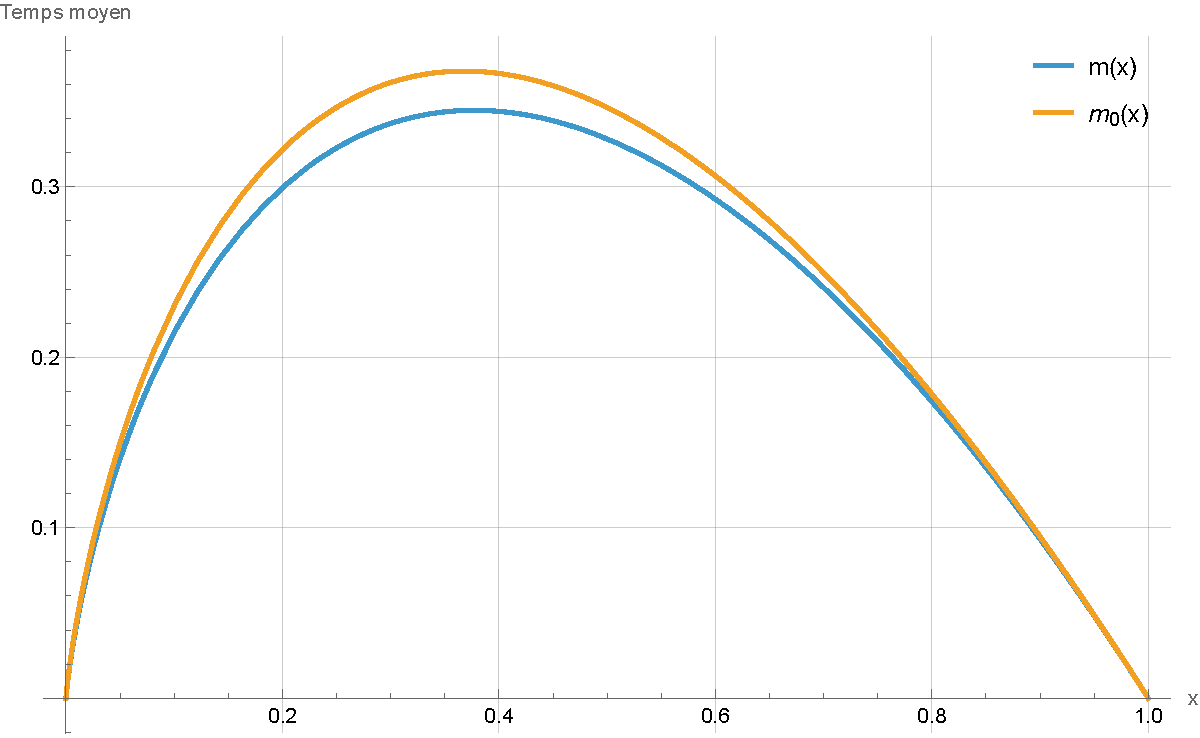
\includegraphics[width=\linewidth]{img/validation/Jumps/mean_jumps.pdf}
        \caption{Fréquence des sauts $\lambda=1$}
    \end{subfigure}
    \hfill
    \begin{subfigure}{0.45\linewidth}
        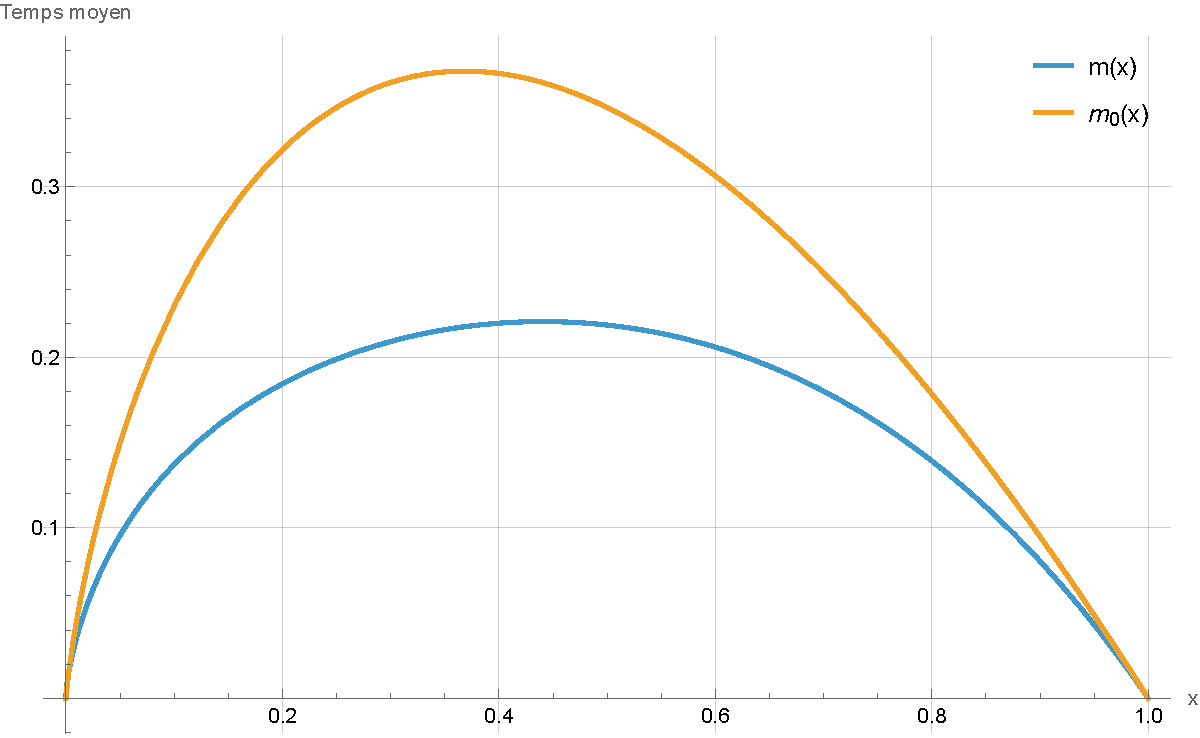
\includegraphics[width=\linewidth]{img/validation/Jumps/mean_big_jumps.pdf}
        \caption{Fréquence des sauts $\lambda=10$}
    \end{subfigure}
    \caption{Visualisation des temps moyens de sortie $m(x)$ et $m_0(x)$}\label{fig:JumpsMeanVisualisation}
\end{figure}
\FloatBarrier\paragraph{Analyse}\phantom{}\\
Il convient de souligner les observations suivantes:
\begin{itemize}
    \item Les conditions aux limites \( m(0) = m(c) = m_0(0) = m_0(c) = 0 \) sont bien vérifiées.
    \item Le temps moyen de sortie en présence de sauts ($m(x)$ en bleu) est inférieur à celui observé sans sauts ($m_0(x)$ en orange), ce qui illustre l'accélération du processus induite par ces derniers.
    \item Une augmentation de la fréquence des sauts $\lambda$ induit une diminution du temps moyen de sortie. Ce comportement est attendu comme les sauts augmente la probabilité que le \acs{CIR} quitte l'intervalle rapidement.
\end{itemize}

\subsection{Fonction Probabilité de sortie en zéro \textemdash~Sauts uniformes}
Les paramètres considérés sont ceux définis dans l'étude de la probabilité de sortie en zéro, présentée en sous-partie (\ref{subsection_probability_jumps}). Les fonctions \( p(x) \) (avec sauts) et \( p_0(x) \) (sans sauts), correspondant respectivement aux expressions (\ref{sol_probability_with_jumps}) et (\ref{sol_probability}), sont représentées graphiquement.
\paragraph{Visualisation}\phantom{}
\begin{figure}[htb]
    \centering
    \begin{subfigure}{0.45\linewidth}
        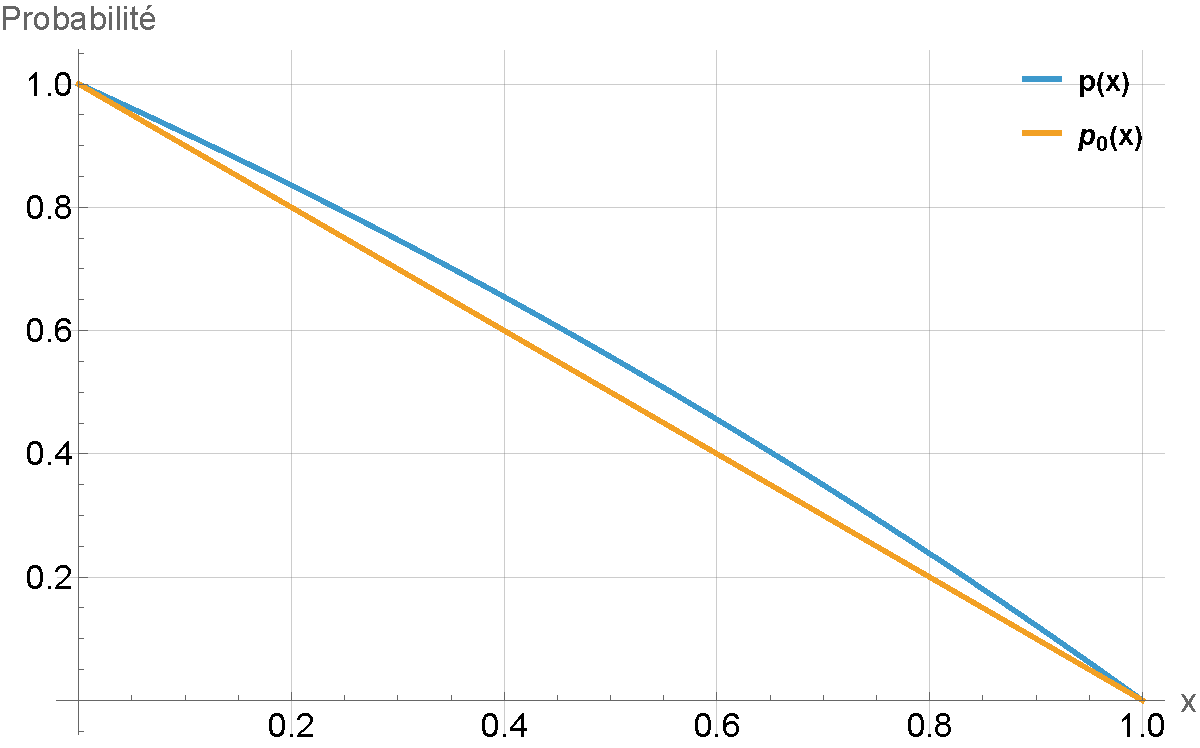
\includegraphics[width=\linewidth]{img/validation/Jumps/probability_jumps.pdf}
        \caption{Fréquence des sauts $\lambda=1$}
    \end{subfigure}
    \hfill
    \begin{subfigure}{0.45\linewidth}
        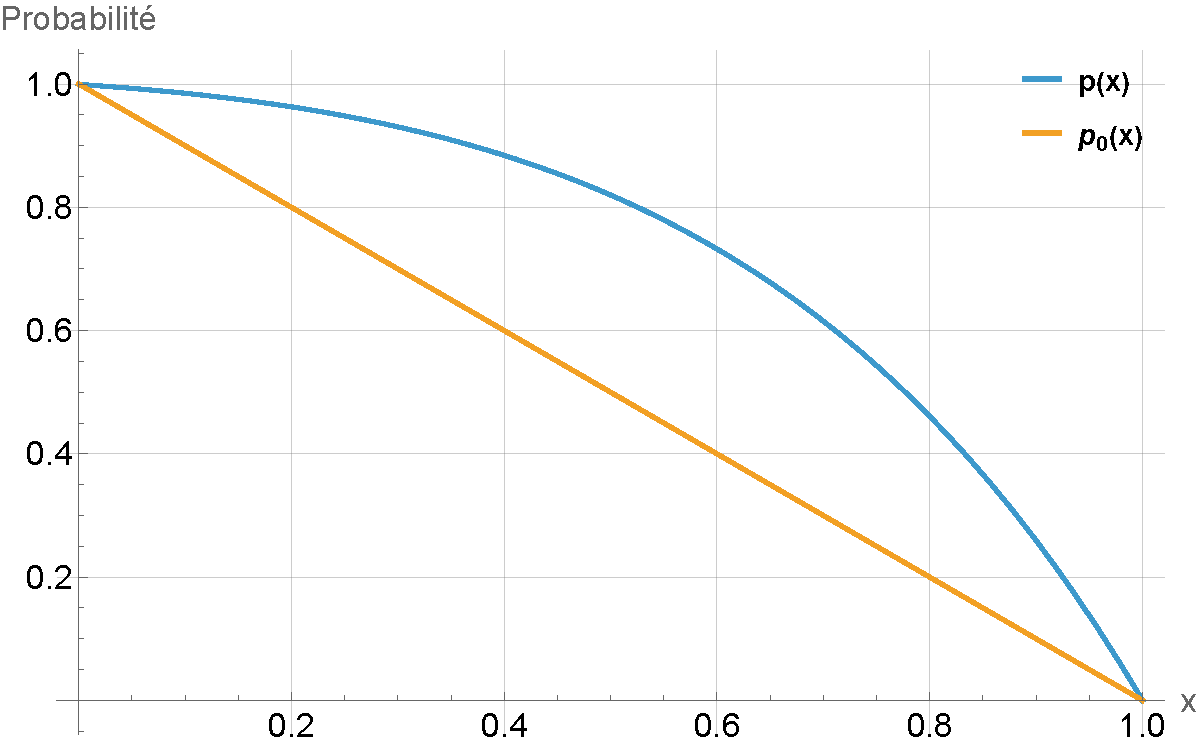
\includegraphics[width=\linewidth]{img/validation/Jumps/probability_big_jumps.pdf}
        \caption{Fréquence des sauts $\lambda=10$}
    \end{subfigure}
    \caption{Visualisation des probabilités de sortir en zéro $p(x)$ et $p_0(x)$}\label{fig:JumpsProbabilityVisualisation}
\end{figure}
\FloatBarrier\paragraph{Analyse}\mbox{}\\
Les observations suivantes peuvent être formulées:
\begin{itemize}
    \item Les conditions aux limites sont correctement satisfaites, à savoir \( p(0) = p_0(0) = 1 \) et \( p(c) = p_0(c) = 0 \).
    \item Les sauts étant négatifs, ils favorisent une sortie par la borne inférieure. La probabilité de franchissement par zéro est donc plus élevée dans le cas avec sauts ($p(x)$ en bleu);
    \item Une augmentation de la fréquence des sauts $\lambda$ entraîne une augmentation considérable de la probabilité de sortir par zéro. En effet, les sauts étant négatifs, leur multiplication tend à entraîner le processus vers la borne inférieure.
\end{itemize}

\subsection{Fonction Dépassement Moyen \textemdash~Sauts exponentiels}
La variante du \acs{CIR} à sauts exponentiels est considérée.
\paragraph{Visualisation}\phantom{}\\
Toujours dans la même optique, la fonction approximative obtenue pour $D(x)$ en (\ref{sol_overshoot}) est tracée pour différentes valeurs de la fréquence des sauts $\lambda$ ainsi que le paramètre de longueur des sauts $\nu$.
\begin{figure}[htb]
    \centering
    \begin{subfigure}{0.45\linewidth}
        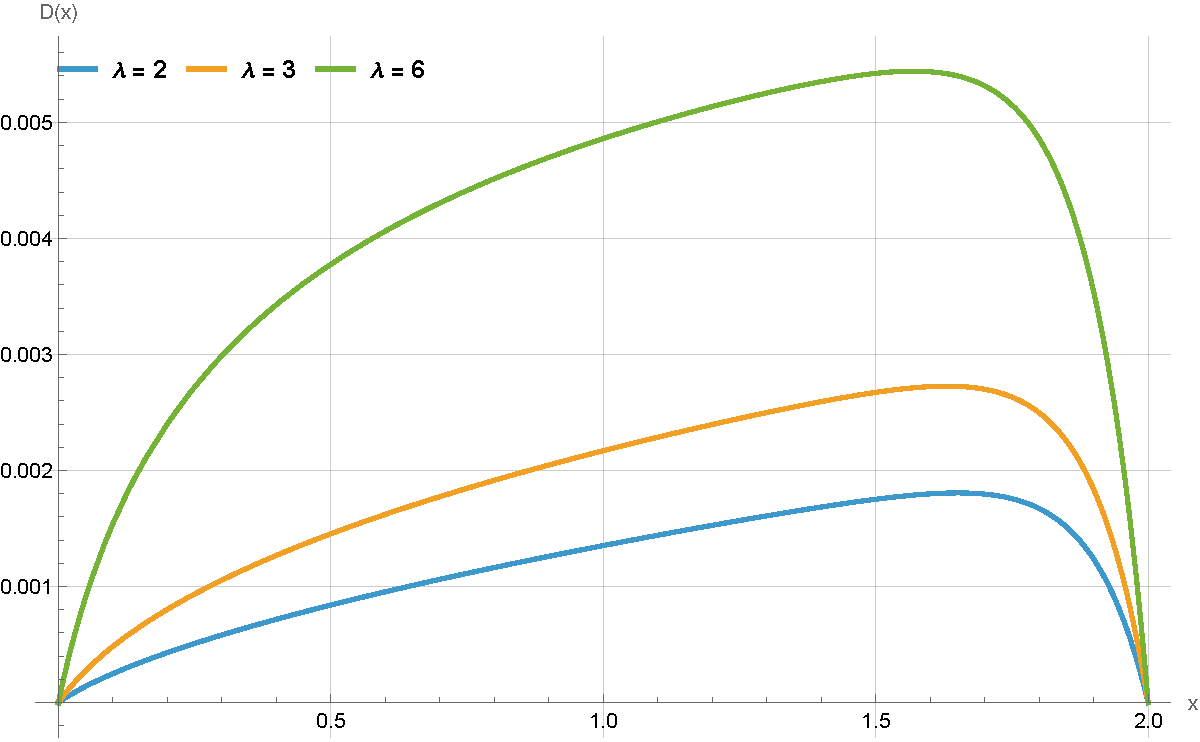
\includegraphics[width=\linewidth]{img/validation/Ovs/overshoot_lambda.pdf}
        \caption{Sensibilité de la fréquence des sauts $\lambda,\;\forall\;\lambda\in\{2,3,6\}$}\label{fig:Overshoot_lambda_visualisation}
    \end{subfigure}
    \hfill
    \begin{subfigure}{0.45\linewidth}
        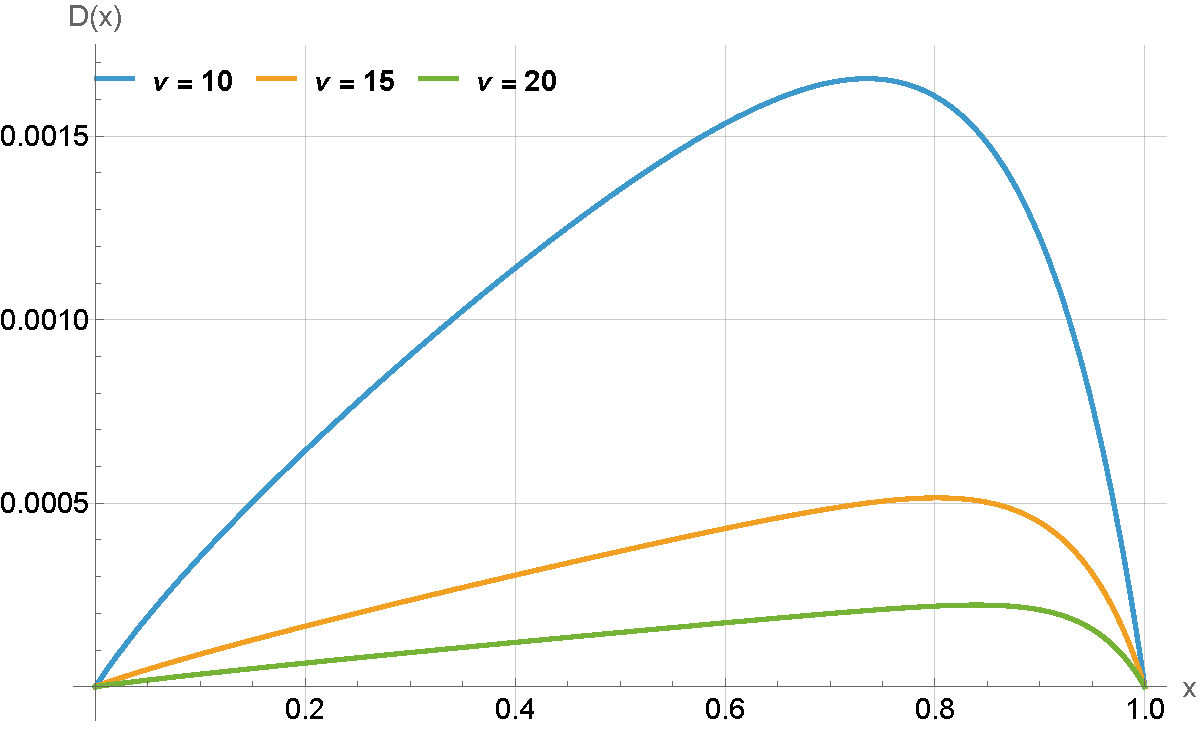
\includegraphics[width=\linewidth]{img/validation/Ovs/overshoot_nu.pdf}
        \caption{Sensibilité de la taille des sauts $\nu,\;\forall\;\nu\in\{5,10,15\}$}\label{fig:Overshoot_nu_visualisation}
    \end{subfigure}
    \hfill
    \caption{Visualisation de la fonction Dépassement Moyen $D(x)$}\label{fig:OvershootVisualisation}
\end{figure}
\FloatBarrier\paragraph{Analyse}\phantom{}\\
Les différents points suivants sont relevés:
\begin{itemize}
    \item Les conditions aux limites $D(0)=D(c)=0$ sont respectées;
    \item La fonction représente un \textit{dépassement moyen}, elle doit donc être positive pour toute valeur $x$ dans $[0,c]$;
    \item Une augmentation de la fréquence des sauts $\lambda$ induit une augmentation du dépassement moyen. En effet, il devient plus probable que le processus effectue un saut juste avant d'atteindre la frontière, ce qui augmente les chances de la franchir avec un certain excès.
    \item Une réduction de la taille des sauts (traduite par une augmentation de $\nu$) induit une diminution du dépassement moyen. En effet, même si un saut survient à proximité de la frontière, sa faible amplitude limite la distance franchie au-delà de celle-ci.
\end{itemize}

             % Second thème (Doctorat) ou "Résultats théoriques et expérimentaux" (Maîtrise) / Second theme (PhD) or "Theoretical and experimental results" (Master's)
\Chapter{PREMIER PASSAGE EN DIFFUSION PURE}\label{sec:FPT_Diffusion}

Cette partie du mémoire est consacrée à la résolution analytique des problèmes de premier passage appliqués au processus \acl{CIR} en diffusion pure.

\section{Fonction Génératrice des Moments}\label{section_fgm_eq}
\subsection{Résolution du problème}
\paragraph{Dérivation de l'équation à résoudre}\phantom{}\\
Soit un processus d'Itô défini par l'\ac{EDS} (\ref{ito_eq}).
Il est connu que la \acl{FGM} d'un temps de premier passage $\tau(x)$ satisfait l'équation du passé de Kolmogorov (voir~\cite{cox2017} ou~\cite{lefebvre2007}): 
\[
\frac{1}{2}\sigma{(t,x)}^2M''(x;\alpha)+\mu(t,x)M'(x;\alpha)-\alpha M(x;\alpha)=0
\]
avec $M(0;\alpha)=M(c;\alpha)=1$. 

En reprenant les termes de dérive et de diffusion du \acs{CIR} (\ref{cir_eq}), l'\ac{EDO} linéaire de second ordre à résoudre devient: 
\begin{equation}\label{ode_fgm}
    \frac{1}{2}\sigma^2xM''(x;\alpha)+a(b-x)M'(x;\alpha)-\alpha M(x;\alpha)=0
\end{equation}

\paragraph{Résolution}\phantom{}\\
D'abord, en multipliant les deux côtés par $2/\sigma^2$ l'équation ci-dessus (\ref{ode_fgm}) est mise sous forme canonique: 
\[
xM''(x;\alpha)-\left(\frac{2a}{\sigma^2}x-\frac{2ab}{\sigma^2}\right)M'(x;\alpha)-\frac{2\alpha}{\sigma^2} M(x;\alpha)=0
\]
Ensuite, un changement de variable $y=\beta x$ avec $M(x;\alpha)=G(y;\alpha)$ est introduit. L'équation devient: 
\[
yG''(y;\alpha)-\left(\frac{2a}{\sigma^2} \beta y - \frac{2ab}{\sigma^2}\right)G'(y;\alpha)-\beta\frac{2\alpha}{\sigma^2} G(y;\alpha) = 0
\]
Ce changement de variable a pour objectif de déterminer, en fonction des autres paramètres du problème, la valeur de $\beta$ qui permet de ramener l'équation à la forme générale de l'équation de Kummer (\ref{kummer_eq}): 
\begin{equation}\label{kummer_eq}
    xf''(x)-(x-\theta)f'(x)-s f(x)=0,\quad\quad \theta,s\in\mathds{R}
\end{equation}
dont la solution est connue. Pour ce faire, il faut que:
\[
\frac{2a}{\sigma^2} \beta=1\implies\beta=\frac{\sigma^2}{2a}
\]
L'équation devient:
\begin{equation}\label{kummer_eq2}
    yG''(y;\alpha)-\left(y-\frac{2ab}{\sigma^2}\right)G'(y;\alpha)-\frac{\alpha}{a}G(y;\alpha) = 0
\end{equation}
La solution générale de cette dernière (\ref{kummer_eq2}) est de la forme (voir~\cite{magnus1966}): 
\[G(y;\alpha) = C_1\Phi\left(\frac{\alpha}{a}, \frac{2ab}{\sigma^2}, y\right) + C_2\Psi\left(\frac{\alpha}{a}, \frac{2ab}{\sigma^2}, y\right)\]
avec $C_1$ et $C_2$ des constantes à déterminer, et $\Phi(\cdot, \cdot, \cdot)$ et $\Psi(\cdot, \cdot, \cdot)$ sont les fonctions hypergéométriques confluentes de première et seconde espèce (voir annexe~\ref{special_functions}).

Finalement, l'expression analytique de la \acs{FGM} de $\tau(x)$ est: 
\begin{equation}\label{sol_fgm}
    M(x;\alpha) = C_1\Phi\left(\frac{\alpha}{a}, \frac{2ab}{\sigma^2}, \frac{2ax}{\sigma^2}\right) + C_2\Psi\left(\frac{\alpha}{a}, \frac{2ab}{\sigma^2}, \frac{2ax}{\sigma^2}\right)
\end{equation}

\paragraph{Détermination des constantes}\phantom{}\\
Les conditions aux limites $M(0;\alpha)=M(c;\alpha)=1$ permettent de déterminer les deux constantes $C_1$ et $C_2$ en résolvant le système suivant:
\[
\begin{cases}
    C_1\Phi\left(\frac{\alpha}{a}, \frac{2ab}{\sigma^2}, 0\right) + C_2\Psi\left(\frac{\alpha}{a}, \frac{2ab}{\sigma^2}, 0\right) = 1 \\
C_1\Phi\left(\frac{\alpha}{a}, \frac{2ab}{\sigma^2}, \frac{2ac}{\sigma^2}\right) + C_2\Psi\left(\frac{\alpha}{a}, \frac{2ab}{\sigma^2}, \frac{2ac}{\sigma^2}\right) = 1
\end{cases}
\]
Il en découle les valeurs suivantes pour $C_1$ et $C_2$: 
\begin{equation}\label{fgm_constants}
    \begin{aligned}
        &C_1 = \frac{\Phi(\frac{\alpha}{a}, \frac{2ab}{\sigma^2}, 0)-\Psi(\frac{\alpha}{a}, \frac{2ab}{\sigma^2}, 0)}{\Phi(\frac{\alpha}{a}, \frac{2ab}{\sigma^2}, \frac{2ac}{\sigma^2})\Psi(\frac{\alpha}{a}, \frac{2ab}{\sigma^2}, 0)-\Psi(\frac{\alpha}{a}, \frac{2ab}{\sigma^2}, \frac{2ac}{\sigma^2})} \\
        &C_2 = \frac{\Phi(\frac{\alpha}{a}, \frac{2ab}{\sigma^2}, \frac{2ac}{\sigma^2})-1}{\Phi(\frac{\alpha}{a}, \frac{2ab}{\sigma^2}, \frac{2ac}{\sigma^2})\Psi(\frac{\alpha}{a}, \frac{2ab}{\sigma^2}, 0)-\Psi(\frac{\alpha}{a}, \frac{2ab}{\sigma^2}, \frac{2ac}{\sigma^2})}
    \end{aligned}
\end{equation}
\subsection{Validation de l'expression obtenue}
\paragraph{Visualisation}\phantom{}\\
Il convient de valider le comportement de la \acl{FGM} $M(x;\alpha)$ définie par (\ref{sol_fgm},~\ref{fgm_constants}). À cet effet, il faut tracer son évolution sur l'intervalle $[0, c]$ pour plusieurs valeurs du paramètre $\alpha \in \{1, 2, 5, 10\}$. Concernant les paramètres du \acs{CIR} (\ref{cir_eq}), et sauf indication contraire, les valeurs utilisées pour l'ensemble des visualisations sont:
\begin{itemize}
    \item Vitesse de retour: \(a=0.1\);
    \item Moyenne long-terme: \(b=0.9\);
    \item Volatilité infinitésimale: \(\sigma=1\).
\end{itemize}
\begin{figure}[htb]
    \centering
    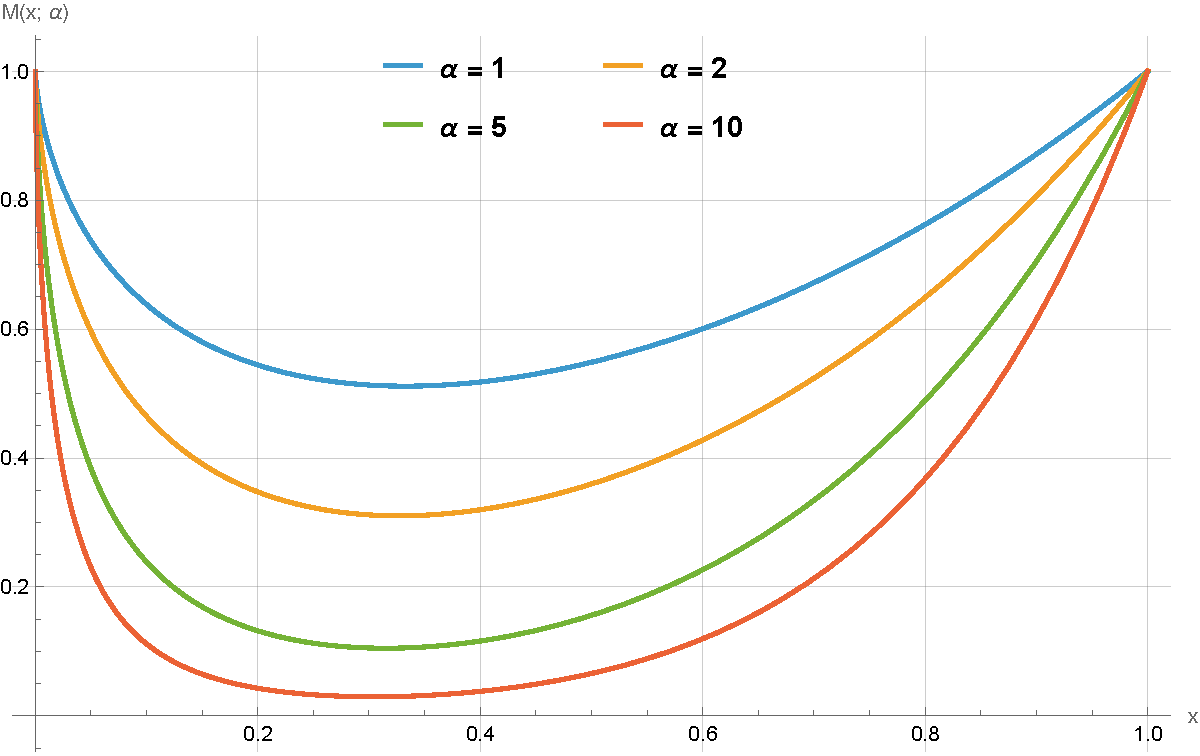
\includegraphics[width=0.5\linewidth]{img/validation/fgm.pdf}
    \caption{Visualisation de la \acl{FGM} $M(x;\alpha)$}\label{fig:FGMVisualisation}
\end{figure}
\FloatBarrier\paragraph{Analyse}\phantom{}\\
Il est important de souligner les points suivants:
\begin{itemize}
    \item Les conditions aux limites $M(0; \alpha) = M(c; \alpha) = 1$ sont respectées;
    \item Puisque $\alpha$ est par définition un paramètre positif (\ref{fgm}), la fonction est bien comprise dans l'intervalle $(0, 1)$, car elle correspond à l'exponentielle d'un nombre négatif;
    \item Par ailleurs, et pour la même raison, lorsque $\alpha$ augmente, la fonction diminue.
\end{itemize}
L'expression obtenue pour la \acl{FGM} est ainsi validée. 

\section{Fonction Temps Moyen}\label{section_mean_eq}
\subsection{Résolution du problème}
\paragraph{Dérivation de l'équation à résoudre}\phantom{}\\
En combinant le développement en série entière de l'exponentielle: 
\[
e^x=\sum_{k=0}^\infty\frac{x^k}{k!}
\]
et la définition de la \acl{FGM} (\ref{fgm}), il est possible d'écrire (en supposant que les moments de $\tau(x)$ existent et sont finis): 
\begin{equation}\label{taylor_fgm}
    \begin{aligned}
        M(x;\alpha)=\mathds{E}\left[e^{-\alpha \tau(x)}\right]&=\mathds{E}\left[\sum_{k=0}^\infty\frac{{(-\alpha\tau(x))}^k}{k!}\right] \\
        &= \sum_{k=0}^\infty\frac{{(-\alpha)}^k\mathds{E}\left[{\tau(x)}^k\right]}{k!}\\
        &=1-\alpha\mathds{E}[\tau(x)]+\frac{\alpha^2}{2}\mathds{E}\left[{\tau(x)}^2\right]-\ldots
    \end{aligned}
\end{equation}
En injectant (\ref{taylor_fgm}) dans l'équation (\ref{ode_fgm}), et en reprenant la définition (\ref{mean}), il découle l'\acs{EDO} linéaire de second ordre suivante: 
\begin{equation}\label{ode_mean}
    \frac{1}{2}\sigma^2xm''(x)+a(b-x)m'(x)=-1   
\end{equation}
avec $m(0)=m(c)=0$. En résolvant cette équation, une expression analytique de la fonction temps moyen est obtenue. 

\paragraph{Réduction d'ordre}\phantom{}\\
D'abord, afin d'alléger la notation, soit:
\begin{equation}\label{notation}
\begin{cases}
    \alpha = \frac{2a}{\sigma^2} \\
    \beta=\frac{2ab}{\sigma^2} \\
    \theta=-\frac{2}{\sigma^2}
\end{cases}
\end{equation}
L'équation peut donc être réécrite comme suit: 
\begin{equation}\label{simplified_ode_mean}
    xm''(x)+(\beta-\alpha x)m'(x)=\theta
\end{equation}
La réduction d'ordre $u(x)=m'(x)$ donne l'\acs{EDO} linéaire de premier ordre suivante:
\begin{equation}\label{order_reduction}
xu'(x)+(\beta-\alpha x)u(x)=\theta
\end{equation}
Pour procéder à sa résolution, il faut résoudre l'équation homogène associée puis déduire une solution particulière avec la méthode de variation de la constante. La solution générale obtenue est, avec $C_1$ une constante: 
\begin{equation}\label{sol_first_order_mean}
    u(x)=x^{-\beta}e^{\alpha x}(C_1-\theta \alpha^{-\beta}\Gamma(\beta, \alpha x))
\end{equation}
où $\Gamma(\cdot,\cdot)$ est la fonction Gamma incomplète (voir annexe~\ref{special_functions}).
Il suffit donc d'intégrer $u(x)$ et d'ajouter une constante $C_2$ pour obtenir l'expression de $m(x)$: 
\begin{equation}\label{intergration_sol_first_order}
    m(x)=\int u(x)dx+C_2
\end{equation}
Cependant, un problème survient lors de l'intégration du terme:
\begin{equation}\label{problematic_integral}
    \int\theta \underbrace{\phantom{|}{(\alpha x)}^{-\beta}\phantom{|}}_{P}\underbrace{\phantom{|}e^{\alpha x}\phantom{|}}_{E}\underbrace{\phantom{|}\Gamma(\beta, \alpha x)\phantom{|}}_{G}dx
\end{equation}
dans l'expression de $u(x)$ donnée par (\ref{sol_first_order_mean}). En effet, cette intégrale ne possède pas de solution analytique. Les logiciels de calcul symbolique tels que \textit{Mathematica} ou \textit{Maple} échouent également à en trouver une. Il est donc nécessaire d'explorer une autre approche afin de contourner cette difficulté.
\paragraph{Intégration}\phantom{}\\
L'intégrande de (\ref{problematic_integral}) présente des difficultés en raison de la présence du terme puissance $P:={(\alpha x)}^{-\beta}$ multiplié par le terme $E:=e^{\alpha x}$, ainsi que le terme $G:=\Gamma(\beta, \alpha x)$ (lui-même une intégrale). L'objectif est donc de reformuler cette expression afin de simplifier ou d'éliminer certains termes problématiques. C'est précisément ce qui sera abordé dans la suite de cette section. En effet, en combinant les deux expressions suivantes~\cite{NIST:DLMF}: 
\begin{align*}
    \left\{
    \begin{aligned}
        \Gamma(s,x) &= \Gamma(s)-\gamma(s,x) \\
        \gamma(s,x) &= x^s\Gamma(s)e^{-x}\sum_{k=0}^{\infty} \frac{x^k}{\Gamma(s+k+1)}
    \end{aligned}
    \right.
\end{align*}
avec $\gamma(\cdot,\cdot)$ une autre forme de la fonction gamma incomplète (voir annexe~\ref{special_functions}). 

Il est possible d'écrire:
\[
    \Gamma(s,x) = \Gamma(s)-x^s\Gamma(s)e^{-x}\sum_{k=0}^{\infty} \frac{x^k}{\Gamma(s+k+1)}
\]
et donc, en reprenant les termes de l'équation à résoudre (\ref{notation}) il découle l'expression suivante: 
\begin{equation}\label{incomplete_gamma_simplification}
    \Gamma(\beta, \alpha x) = \Gamma(\beta)-\Gamma(\beta)\underbrace{\phantom{|}{(\alpha x)}^\beta\phantom{|}}_{P'} \underbrace{\phantom{|}e^{-\alpha x}\phantom{|}}_{E'}\sum_{k=0}^{\infty} \frac{{(\alpha x)}^k}{\Gamma(\beta+k+1)}
\end{equation}
L'expression ci-dessus (\ref{incomplete_gamma_simplification}) est très intéressante. En effet, en remplaçant le terme $G$ dans (\ref{problematic_integral}) par (\ref{incomplete_gamma_simplification}), les termes $P$ et $P'$ ainsi que $E$ et $E'$ se simplifient comme suit:
\[
    \begin{aligned}
        &\int\theta \underbrace{\phantom{|}{(\alpha x)}^{-\beta}\phantom{|}}_{P}\underbrace{\phantom{|}e^{\alpha x}\phantom{|}}_{E}\overbrace{\left(\Gamma(\beta)-\Gamma(\beta)\underbrace{\phantom{|}{(\alpha x)}^\beta\phantom{|}}_{P'} \underbrace{\phantom{|}e^{-\alpha x}\phantom{|}}_{E'}\sum_{k=0}^{\infty} \frac{{(\alpha x)}^k}{\Gamma(\beta+k+1)}\right)}^{G}dx \\
        &= \int\theta\Gamma(\beta)\underbrace{\phantom{|}{(\alpha x)}^{-\beta}\phantom{|}}_{P}\underbrace{\phantom{|}e^{\alpha x}\phantom{|}}_{E}dx-\int\theta\Gamma(\beta)\underbrace{\phantom{|}{(\alpha x)}^{-\beta}\phantom{|}}_{P}\underbrace{\phantom{|}{(\alpha x)}^\beta\phantom{|}}_{P'}\underbrace{\phantom{|}e^{\alpha x}\phantom{|}}_{E} \underbrace{\phantom{|}e^{-\alpha x}\phantom{|}}_{E'}\sum_{k=0}^{\infty} \frac{{(\alpha x)}^k}{\Gamma(\beta+k+1)} \\
        &= \int\theta\Gamma(\beta)\underbrace{\phantom{|}{(\alpha x)}^{-\beta}\phantom{|}}_{P}\underbrace{\phantom{|}e^{\alpha x}\phantom{|}}_{E}dx-\theta\Gamma(\beta)\int\sum_{k=0}^{\infty} \frac{{(\alpha x)}^k}{\Gamma(\beta+k+1)}
    \end{aligned}
\]
En injectant dans (\ref{intergration_sol_first_order}), il découle: 
\[
m(x)=(C_1-\theta\alpha^{-\beta}\Gamma(\beta))\underbrace{\int x^{-\beta}e^{\alpha x}dx}_I + \,\theta\Gamma(\beta) \underbrace{\int\sum_{k=0}^{\infty} \frac{{(\alpha x)}^k}{\Gamma(\beta+k+1)}dx}_J + C_2
\]
avec $I$ et $J$ deux intégrales à résoudre: 
\begin{itemize}
    \item \textbf{Résolution de} $I$: \\
    \textit{Wolfram Mathematica} donne:
    \begin{equation}\label{exponential_integral}
        \int x^{-\beta}e^{\alpha x}dx = -x^{1-\beta}E_\beta(-\alpha x)
    \end{equation}
    où $E_n(x)$ est la fonction intégrale exponentielle généralisée (voir annexe~\ref{special_functions}).
    La relation suivante~\cite{abramowitz1964}:
    \[
    E_n(x)=x^{n-1}\Gamma(1-n,x)
    \]
    permet d'écrire: 
    \begin{equation}\label{exponential_integral_simplification}
        E_{\beta}(-\alpha x)={(-\alpha x)}^{\beta-1}\Gamma(1-\beta,-\alpha x)
    \end{equation}
    En combinant (\ref{exponential_integral}) et (\ref{exponential_integral_simplification}), l'expression analytique de la solution de $I$ est obtenue:
    \[
        I=-{(-\alpha)}^{\beta-1}\Gamma(1-\beta,-\alpha x)
    \]
    \item \textbf{Résolution de $J$}: \\
    La série à l'intérieur de l'intégrale converge uniformément grâce au terme factoriel au dénominateur. L'intégration terme-à-terme est donc possible: 
    \[
    \begin{aligned}
        \int\sum_{k=0}^{\infty} \frac{{(\alpha x)}^k}{\Gamma(\beta+k+1)}dx &= \sum_{k=0}^{\infty} \int \frac{{(\alpha x)}^k}{\Gamma(\beta+k+1)}dx \\
        &= \sum_{k=0}^{\infty} \frac{\alpha^k x^{k+1}}{(k+1)\Gamma(\beta+k+1)} \\
        &= \frac{x}{\Gamma(1+\beta)}\,_2F_2\left(\begin{bmatrix}1\\1\end{bmatrix},\begin{bmatrix}2\\1+\beta\end{bmatrix},\alpha x\right)
    \end{aligned}
    \]
    où $_p F_q(\cdot,\cdot,\cdot)$ est la fonction hypergéométrique généralisée (voir annexe~\ref{special_functions}).
    
\end{itemize}
La forme finale de l'expression de la fonction temps moyen est donc:
\begin{equation}\label{sol_mean}
    m(x)={(-\alpha)}^{\beta-1}\Gamma(1-\beta,-\alpha x)\left[\theta\alpha^{-\beta}\Gamma(\beta)-C_1\right]+\frac{\theta x}{\beta}\,{}_2F_2\left(\begin{bmatrix}1\\1\end{bmatrix},\begin{bmatrix}2\\1+\beta\end{bmatrix},\alpha x\right) + C_2
\end{equation}

\paragraph{Détermination des constantes}\phantom{}\\
Les conditions aux limites $m(0)=m(c)=0$ permettent de déterminer les deux constantes $C_1$ et $C_2$ en résolvant le système suivant: 
\begin{align*}
\left\{\begin{aligned}
(\theta\alpha^{-\beta}\Gamma(\beta)-C_1)\alpha^{\beta-1}\Gamma(1-\beta) + C_2 &= 0\\
(\theta\alpha^{-\beta}\Gamma(\beta)-C_1)\alpha^{\beta-1}\Gamma(1-\beta,\alpha c) + \frac{c\theta}{\beta}\,{}_2F_2\left(\begin{bmatrix}1\\1\end{bmatrix},\begin{bmatrix}2\\1+\beta\end{bmatrix},\alpha c\right)+ C_2 &= 0
\end{aligned}\right. \\
\end{align*}
Les expressions des constantes $C_1$ et $C_2$ sont donc:
\begin{equation}\label{mean_constants}
    \begin{aligned}
        C_1 &= \alpha^{-\beta}\theta\Gamma(\beta)+\frac{\alpha c \theta {(-\alpha)}^{-\beta}}{\beta\gamma(1-\beta,\alpha c)}\,{}_2F_2\left(\begin{bmatrix}1\\1\end{bmatrix},\begin{bmatrix}2\\1+\beta\end{bmatrix},\alpha c\right) \\
        C_2 &= -\frac{c\theta\Gamma(1-\beta)}{\beta\gamma(1-\beta,\alpha c)}\,{}_2F_2\left(\begin{bmatrix}1\\1\end{bmatrix},\begin{bmatrix}2\\1+\beta\end{bmatrix},\alpha c\right)
    \end{aligned}
\end{equation}
avec $\alpha$, $\beta$ et $\theta$ définis en (\ref{notation}).
\subsection{Validation de l'expression obtenue}

\paragraph{Visualisation}\phantom{}\\
Enfin, il est nécessaire de valider le comportement de la fonction Temps Moyen $m(x)$ définie par (\ref{sol_mean},~\ref{mean_constants}). La fonction est donc tracée pour différentes valeurs des paramètres $a,\;\forall\;a\in\{0.1,0.2,0.4\}$ et $\sigma,\;\forall\;\sigma\in\{1,\sqrt{2},2\}$.


\begin{figure}[htb]
    \centering
    \begin{subfigure}{0.45\linewidth}
        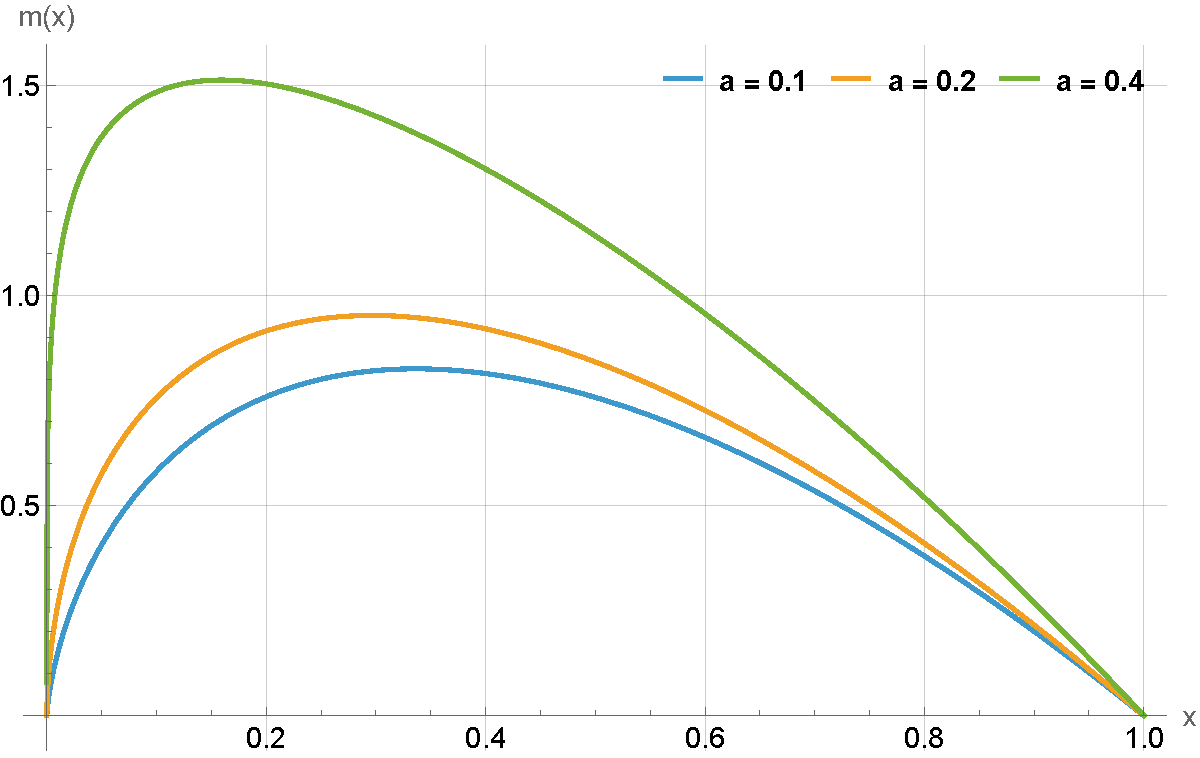
\includegraphics[width=\linewidth]{img/validation/Mean/mean_a.pdf}
        \caption{Sensibilité de la vitesse $a$}\label{fig:Mean_a_visualisation}
    \end{subfigure}
    \hfill
    \begin{subfigure}{0.45\linewidth}
        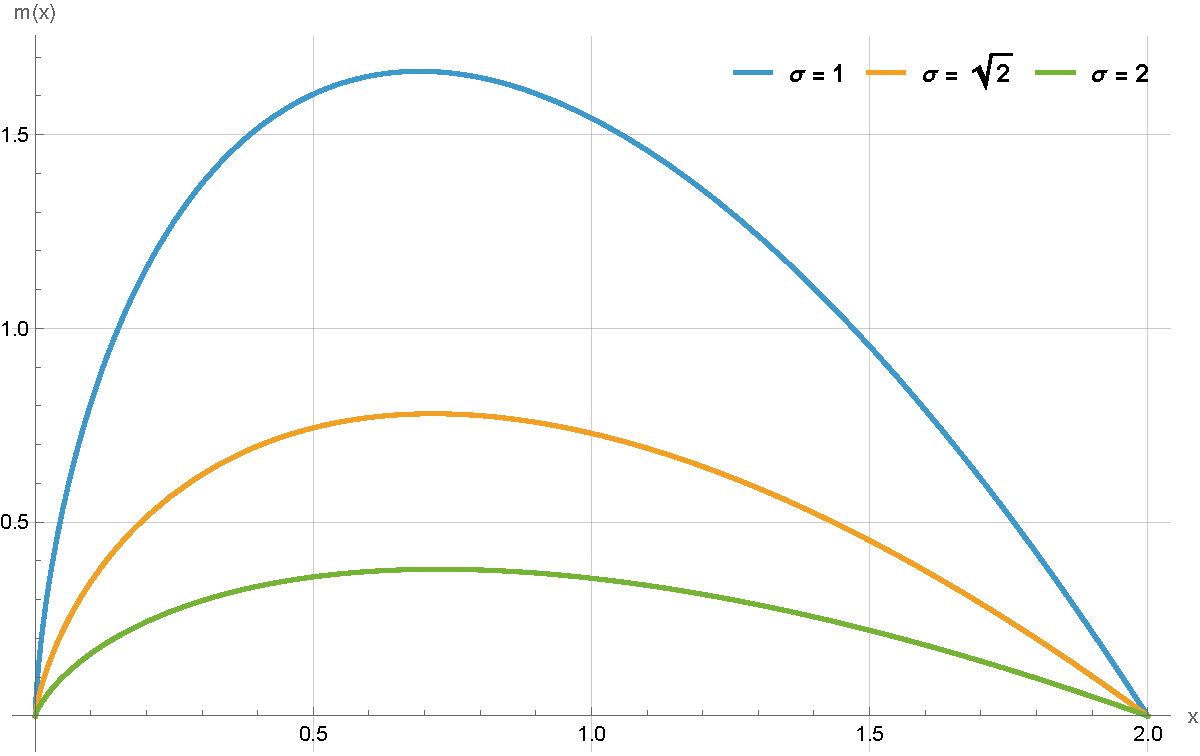
\includegraphics[width=\linewidth]{img/validation/Mean/mean_sigma.pdf}
        \caption{Sensibilité de la volatilité infinitésimale $\sigma$}\label{fig:Mean_sigma_visualisation}
    \end{subfigure}
    \caption{Visualisation de la fonction Temps Moyen $m(x)$}\label{fig:MeanVisualisation}
\end{figure}
\FloatBarrier\paragraph{Analyse}\phantom{}\\
Il est important de noter les points suivants:
\begin{itemize}
    \item Les conditions aux limites $m(0)=m(c)=0$ sont respectées;
    \item Cette fonction représente un \textit{temps moyen de premier passage}, elle doit donc être positive pour toute valeur de $x$ dans $[0,c]$;
    \item Une augmentation de la vitesse de retour $a$ entraîne une hausse du temps moyen de sortie de l'intervalle. En effet, plus la force de rappel vers la moyenne est forte (i.e., $a$ élevé), plus une déviation significative et peu probable est nécessaire pour franchir les bornes de l'intervalle;
    \item À l'inverse, une augmentation de la volatilité infinitésimale $\sigma$ diminue le temps moyen de sortie. Cela s'explique naturellement: des fluctuations plus intenses accroissent la probabilité de quitter rapidement l'intervalle.
\end{itemize}

L'expression obtenue pour la fonction de temps moyen de premier passage est ainsi validée.

\section{Fonction Aire Moyenne}
\subsection{Résolution du problème}
\paragraph{Dérivation de l'équation à résoudre}\phantom{}\\
Il est connu que l'\acs{EDO} de second ordre régissant la fonction (\ref{area}) est (voir~\cite{abundo2013}): 
\[\frac{1}{2}\sigma^2xA''(x)+a(b-x)A'(x)=-x\]
En reprenant les notations introduites en (\ref{notation}), l'équation devient: 
\[xA''(x)+(\beta-\alpha x)A'(x)=\theta x\]
Il convient de noter que cette équation ressemble beaucoup à celle dérivée en (\ref{simplified_ode_mean}). La résolution se fera donc de manière semblable.
\paragraph{Réduction d'ordre}\phantom{}\\
En procédant de façon identique à la résolution de l'équation du temps moyen (\ref{order_reduction},~\ref{sol_first_order_mean},~\ref{intergration_sol_first_order}), il est possible d'écrire: 
\[xu'(x)+(\beta-\alpha x)u(x)=\theta x\]
et donc: 
\[u(x)=C_1x^{-\beta} e^{\alpha x} -\theta\alpha^{-\beta-1}x^{-\beta} e^{\alpha x}\Gamma(\beta+1, \alpha x)\]
En combinant l'expression dérivée précédemment (\ref{incomplete_gamma_simplification}) et l'identité suivante~\cite{NIST:DLMF}: 
\[\Gamma(s+1, x)=s\Gamma(s, x)+x^s e^{-x}\]
il est possible de réécrire la solution sous la forme: 
\[
u(x)=C_1x^{-\beta} e^{\alpha x} -\theta\alpha^{-\beta-1}\left(\beta x^{-\beta}e^{\alpha x}\Gamma(\beta)\left(1-{(\alpha x)}^\beta e^{-\alpha x}\sum_{k=0}^{\infty} \frac{{(\alpha x)}^k}{\Gamma(\beta+k+1)}\right)+1\right)
\]

\paragraph{Intégration}\phantom{}\\
Pour obtenir la forme explicite de $A(x)$, il suffit d'intégrer $u(x)$ et d'ajouter une deuxième constante:
\[
\begin{aligned}
    A(x) &= \int u(x)dx+C_2 \\
    &= (C_1-\theta\alpha^{-\beta-1}\Gamma(\beta+1))\underbrace{\int x^{-\beta}e^{\alpha x}dx}_I +\frac{\theta\beta\Gamma(\beta)}{\alpha}\underbrace{\int\sum_{k=0}^{\infty} \frac{{(\alpha x)}^k}{\Gamma(\beta+k+1)}dx}_J-\theta\alpha^{-\beta-1}x +C_2 \\
\end{aligned}
\]
Les deux intégrales résolues précédemment $I$ et $J$ réapparaissent. En injectant leurs solutions analytiques, la forme finale de l'expression de la fonction Aire Moyenne est obtenue: 
\begin{equation}\label{sol_area}
    \begin{aligned}
            A(x) = {(-\alpha)}^{\beta-1}\Gamma(1-\beta,-\alpha x)[\theta\alpha^{-\beta-1}\Gamma(\beta+1)-C_1]\\+\frac{x\theta}{\alpha}\left[{}_2F_2\left(\begin{bmatrix}1\\1\end{bmatrix},\begin{bmatrix}2\\1+\beta\end{bmatrix},\alpha x\right)-\alpha^{-\beta}\right] +C_2 
    \end{aligned}
\end{equation}


\paragraph{Détermination des constantes}\phantom{}\\
Les conditions aux limites $A(0)=A(c)=0$ nous permettent de déterminer les deux constantes $C_1$ et $C_2$ en résolvant le système suivant: 
\begin{align*}
\left\{\begin{aligned}
    {(-\alpha)}^{\beta-1}\Gamma(1-\beta)(\theta\alpha^{-\beta-1}\Gamma(\beta+1)-C_1)+C_2 &= 0 \\
    {(-\alpha)}^{\beta-1}\Gamma(1-\beta,-\alpha c)[\theta\alpha^{-\beta-1}\Gamma(\beta+1)-C_1]\\+ \frac{c\theta}{\alpha}\left[{}_2F_2\left(\begin{bmatrix}1\\1\end{bmatrix},\begin{bmatrix}2\\1+\beta\end{bmatrix},\alpha c\right)-\alpha^{-\beta}\right] +C_2 &=0
\end{aligned}\right.
\end{align*}
Les constantes $C_1$ et $C_2$ s'écrivent donc: 
\begin{equation}\label{area_constants}
    \begin{aligned}
        C_1 =& \frac{1}{\gamma (1-\beta ,-\alpha c)}\Bigg[\theta  {(-\alpha)}^{-\beta } \alpha ^{-\beta -1} \Bigg\{c \alpha ^{\beta +1} \,{}_2F_2\left(\begin{bmatrix}1\\1\end{bmatrix},\begin{bmatrix}2\\1+\beta\end{bmatrix},\alpha c\right)\\&\quad\quad\quad\quad\quad\quad\quad\quad\quad\quad+
        {(-\alpha)}^{\beta } \Gamma(\beta +1)\gamma (1-\beta ,-c \alpha )-\alpha  c\Bigg\}\Bigg] \\
        C_2 =& -\frac{c \theta  \alpha ^{-\beta -1} \Gamma (1-\beta ) }{\gamma(1-\beta ,-c \alpha )}\left[\alpha ^{\beta } \,{}_2F_2\left(\begin{bmatrix}1\\1\end{bmatrix},\begin{bmatrix}2\\1+\beta\end{bmatrix},\alpha c\right)-1\right]
    \end{aligned}
\end{equation}

\subsection{Validation de l'expression obtenue}
\paragraph{Visualisation}\phantom{}\\
Par ailleurs, la même démarche de validation est effectuée pour la fonction Aire Moyenne $A(x)$ définie par (\ref{sol_area},~\ref{area_constants}).

\begin{figure}[htb]
    \centering
    \begin{subfigure}{0.45\linewidth}
        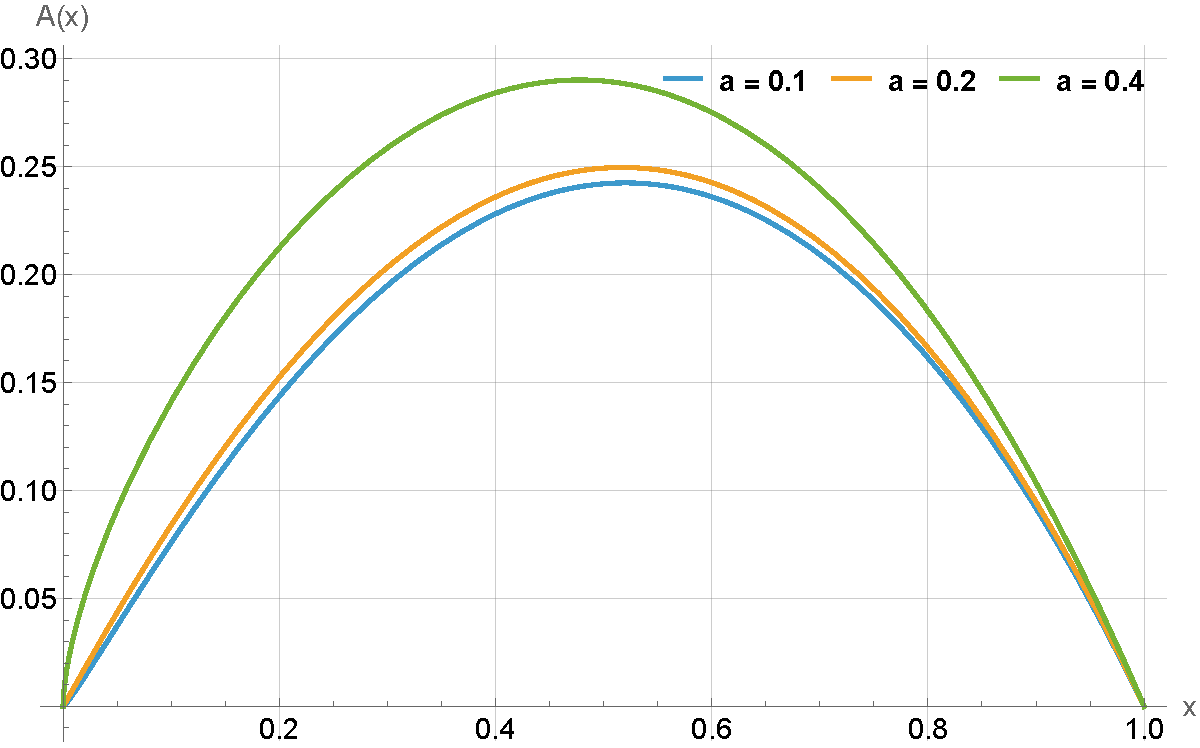
\includegraphics[width=\linewidth]{img/validation/Area/area_a.pdf}
        \caption{Sensibilité de la vitesse $a$}\label{fig:Area_a_visualisation}
    \end{subfigure}
    \hfill
    \begin{subfigure}{0.45\linewidth}
        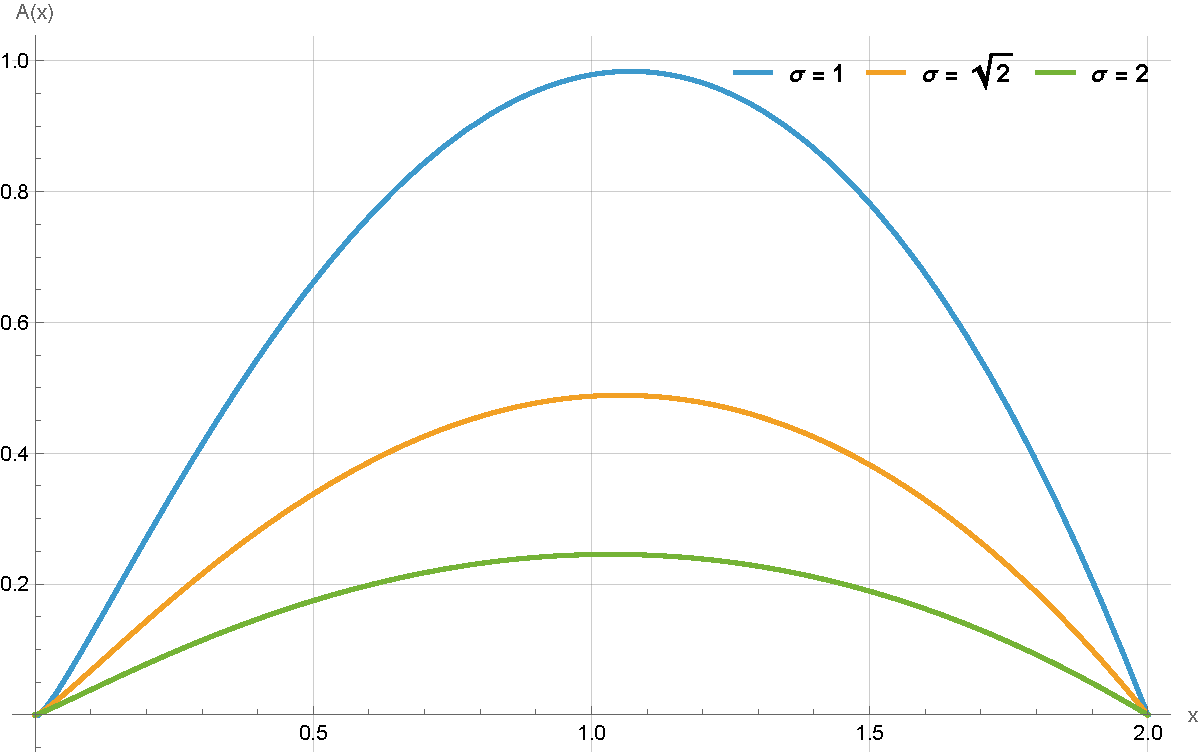
\includegraphics[width=\linewidth]{img/validation/Area/area_sigma.pdf}
        \caption{Sensibilité de la volatilité infinitésimale $\sigma$}\label{fig:Area_sigma_visualisation}
    \end{subfigure}
    \caption{Visualisation de la fonction Aire Moyenne $A(x)$}\label{fig:AreaVisualisation}
\end{figure}
\FloatBarrier\paragraph{Analyse}\phantom{}\\
Il convient de souligner les points suivants:
\begin{itemize}
    \item Les conditions aux limites $A(0)=A(c)=0$ sont respectées;
    \item Cette fonction représente une \textit{aire moyenne} sous un processus positif, elle doit donc être positive pour toute valeur de $x$ dans $[0,c]$;
    \item Une augmentation de la vitesse de retour $a$ entraîne une augmentation de l'aire moyenne sous le processus avant la sortie de l'intervalle. En effet, une force de rappel plus intense maintient le processus autour de sa moyenne plus longtemps, retardant la sortie et augmentant ainsi l'accumulation totale;
    \item À l'inverse, une augmentation de la volatilité infinitésimale $\sigma$ réduit l'aire moyenne. Des fluctuations plus fortes rendent les sorties plus précoces, limitant la durée pendant laquelle le processus peut contribuer à l'intégrale.
\end{itemize}

L'expression obtenue pour la fonction Aire Moyenne est ainsi validée.

\Chapter{PREMIER PASSAGE EN DIFFUSION AVEC SAUTS}\label{sec:FPT_Jump}
Ce chapitre se concentre sur la variante discontinue du \acs{CIR}. Le processus est donc défini comme suit:
\begin{equation}\label{jump_cir_sde}
    X(t)=X(0)+\int_0^t a(b-X(s))ds+\int_0^t\sigma\sqrt{X(s)}dW(s)+J(t)
\end{equation}
avec
\begin{itemize}
    \item $X(0)=x$;
    \item $W(t)$ un \acs{MBS};
    \item $J(t)$ un processus de sauts pur comme défini en (\ref{jump_def}).
\end{itemize}

\section{Fonction Temps moyen \textemdash~Sauts Uniformes Descendants}\label{subsection_mean_jumps}
\subsection{Résolution du problème}
Dans cette section, la variante du \ac{CIR} avec sauts considérée est celle avec des sauts négatifs modélisés par des variables uniformément distribuées sur $[-x,0]$. La mesure d'intensité des sauts est donc:
\[
\gamma(dy)=\lambda\frac{1}{x}\mathds{1}_{y\in[-x,0]}dy
\]

\paragraph{Dérivation de l'équation à résoudre}\phantom{}\\
En reprenant ce qui avait été fait en (\ref{section_fgm_eq}) pour dériver l'\acs{EDO} régissant la \acl{FGM} de $\tau(x)$, il est possible d'écrire:
\[
\frac{1}{2}\sigma^2 xM''(x;\alpha)+a(b-x)M'(x;\alpha)+\lambda\left\{\frac{1}{x}\int_{-x}^0M(x+y;\alpha)dy-M(x;\alpha)\right\}-\alpha M(x;\alpha)=0
\]
avec $M(0;\alpha)=M(c;\alpha)=1$.

Ensuite, en procédant comme dans (\ref{section_mean_eq}), il découle l'équation du temps moyen de sortie de l'intervalle pour le processus avec sauts:
\begin{equation}\label{mean_ide}
    \frac{1}{2}\sigma^2 xm''(x)+a(b-x)m'(x)+\lambda\left\{\frac{1}{x}\int_{-x}^0m(x+y)dy-m(x)\right\}=-1
\end{equation}
avec $m(0)=m(c)=0$.

Soit le changement de variable suivant:
\begin{equation}\label{variable_change_mean}
    \int_{-x}^0m(x+y)dy=\int_0^x m(z)dz
\end{equation}
La formule de Leibniz permet d'écrire:
\[
\frac{d}{dx}\left(\int_0^x m(z)dz\right)=m(x)
\]
Donc, en dérivant les deux côtés de l'équation (\ref{mean_ide}) et en éliminant le retour à la moyenne ($a=0$), il découle une \acs{EDO} d'ordre 3:
\begin{equation}\label{mean_3rd_order}
    \frac{1}{2}\sigma^2xm'''(x)+\sigma^2m''(x)-\lambda m'(x)=-\frac{1}{x}
\end{equation}

\paragraph{Résolution}\phantom{}\\
Soit les valeurs suivantes des paramètres: $\sigma=\sqrt{2}$, $\lambda=1$ et $c=1$. \textit{Maple} donne comme solution:
\begin{equation}\label{sol_mean_with_jumps}
    m(x)=C_1I_0(2\sqrt{x})+C_2K_0(2\sqrt{x})+2\ln(2\sqrt{x})+C_3
\end{equation}
avec $C_1$, $C_2$, $C_3$ des constantes à déterminer et $I_0(\cdot)$, $K_0(\cdot)$ les fonctions de Bessel modifiées de première et seconde espèce respectivement (voir annexe~\ref{special_functions}).

Les constantes $C_1$, $C_2$ et $C_3$ sont déterminées en imposant les conditions aux limites $m(0)=m(1)=0$ ainsi qu'une condition supplémentaire $m(0.5)=r$. Ensuite, la valeur de $r$ permettant de satisfaire l'équation originale (\ref{mean_ide}) est trouvée: $r\simeq0.3281$.

\paragraph{Étude du cas sans sauts}\phantom{}\\
Afin de comparer l'effet de la présence des sauts, il est intéressant de résoudre le même problème en retirant ces derniers. Soit $m_0(x)$ le temps moyen de sortie du processus sans sauts. En considérant les mêmes valeurs des paramètres, l'équation à résoudre devient:
\begin{equation}\label{mean_3rd_order_without_jumps}
    xm_0''(x)=-1
\end{equation}
La solution qui satisfait $m_0(0)=m_0(1)=0$ est:
\begin{equation}\label{sol_mean_with_0_jumps}
    m_0(x)=-x\ln(x)
\end{equation}

\subsection{Validation de l'expression obtenue}
Les fonctions \( m(x) \) (avec sauts) et \( m_0(x) \) (sans sauts), données respectivement par (\ref{sol_mean_with_jumps}) et (\ref{sol_mean_with_0_jumps}), sont tracées.
\paragraph{Visualisation}\phantom{}
\begin{figure}[htb]
    \centering
    \begin{subfigure}{0.45\linewidth}
        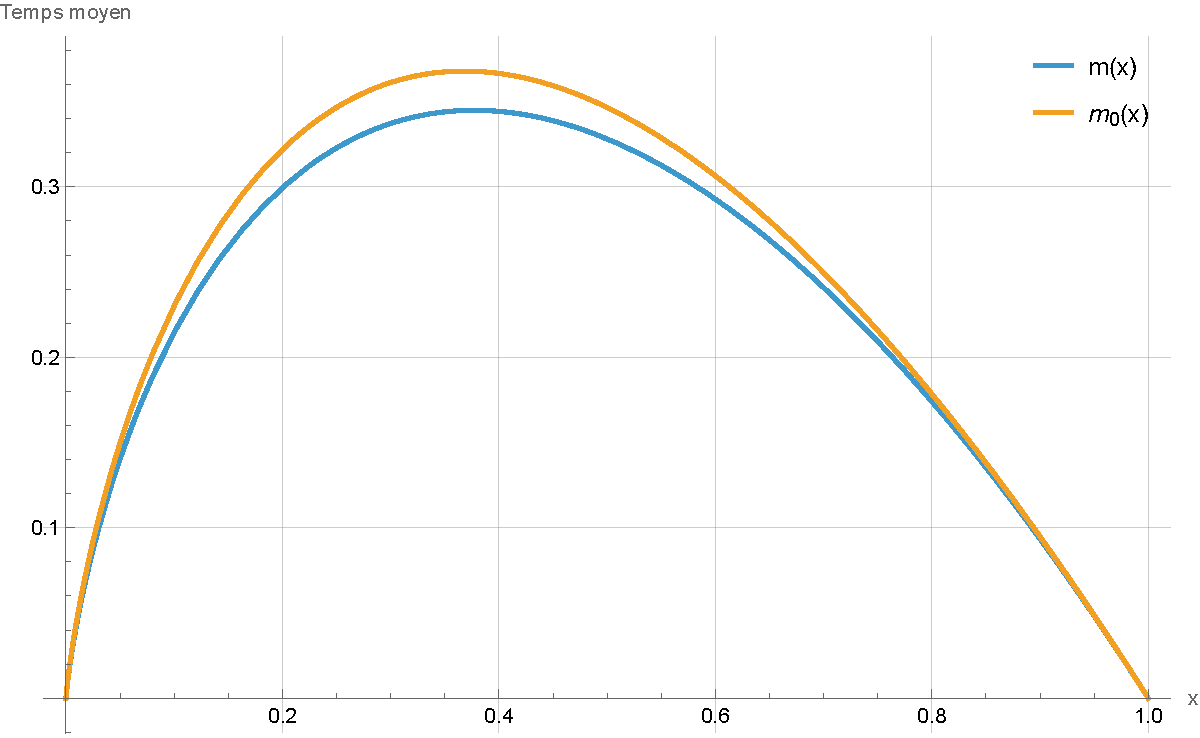
\includegraphics[width=\linewidth]{img/validation/Jumps/mean_jumps.pdf}
        \caption{Fréquence des sauts $\lambda=1$}
    \end{subfigure}
    \hfill
    \begin{subfigure}{0.45\linewidth}
        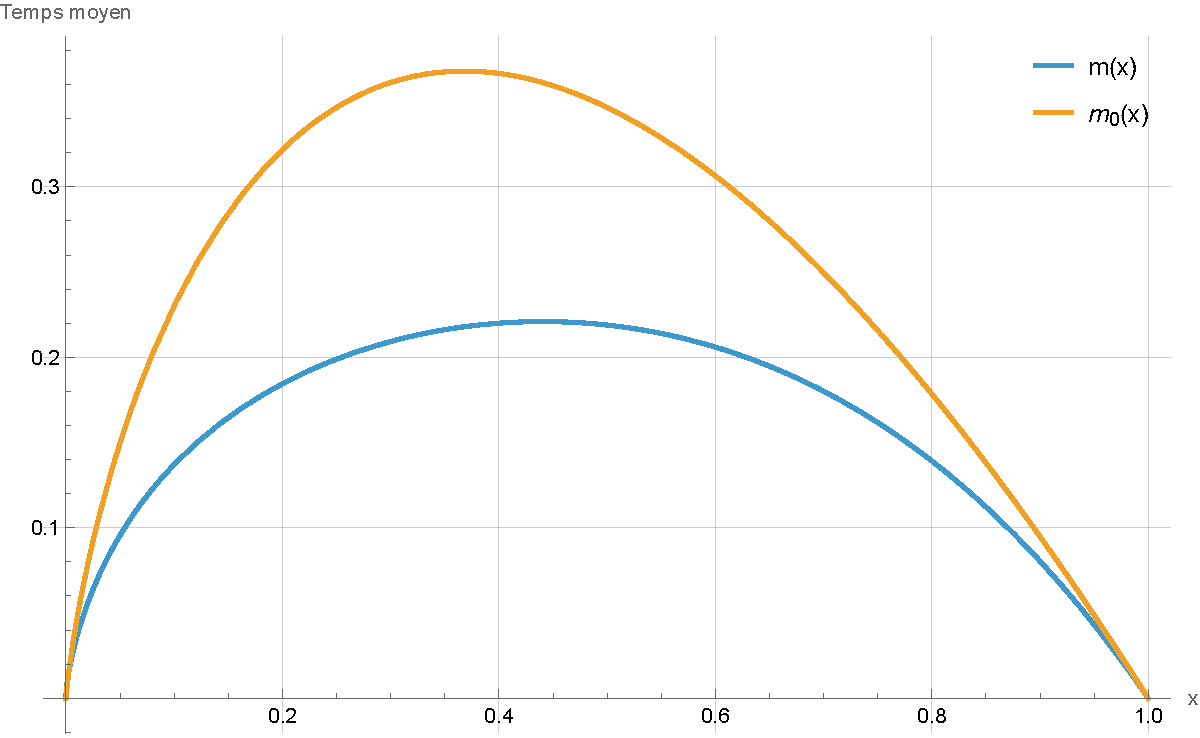
\includegraphics[width=\linewidth]{img/validation/Jumps/mean_big_jumps.pdf}
        \caption{Fréquence des sauts $\lambda=10$}
    \end{subfigure}
    \caption{Visualisation des temps moyens de sortie $m(x)$ et $m_0(x)$}\label{fig:JumpsMeanVisualisation}
\end{figure}
\FloatBarrier\paragraph{Analyse}\phantom{}\\
Il convient de souligner les observations suivantes:
\begin{itemize}
    \item Les conditions aux limites \( m(0) = m(c) = m_0(0) = m_0(c) = 0 \) sont bien vérifiées;
    \item Le temps moyen de sortie en présence de sauts ($m(x)$ en bleu) est inférieur à celui observé sans sauts ($m_0(x)$ en orange), ce qui illustre l'accélération du processus induite par ces derniers;
    \item Une augmentation de la fréquence des sauts $\lambda$ induit une diminution du temps moyen de sortie. Ce comportement est attendu comme les sauts augmente la probabilité que le \acs{CIR} quitte l'intervalle rapidement.
\end{itemize}
La fonction obtenue pour le temps moyen de sortie avec sauts est donc validée.

\section{Fonction Probabilité de sortie en zéro \textemdash~Sauts Uniformes Descendants}\label{subsection_probability_jumps}
\subsection{Résolution du problème}
Dans cette section, la variante du \ac{CIR} avec sauts considérée est identique à la précédente (sauts négatifs modélisés par des variables uniformément distribuées sur $[-x,0]$).

\paragraph{Dérivation de l'équation à résoudre}\phantom{}\\
Il est possible de montrer (voir~\cite{lefebvre2007}) que la fonction probabilité de sortie en zéro satisfait l'\acs{EDO}:
\begin{equation}\label{probability_ide}
    \frac{1}{2}\sigma^2xp''(x)+a(b-x)p'(x)+\lambda\left\{\frac{1}{x}\int_{-x}^0p(x+y)dy-p(x)\right\}=0
\end{equation}
sous les conditions $p(0)=1$ et $p(c)=0$.

Ensuite, en effectuant le même changement de variable que pour la fonction temps moyen (\ref{variable_change_mean}), en dérivant les deux membres de l'équation et en éliminant le retour à la moyenne ($a=0$), il découle:
\begin{equation}\label{probability_3rd_order}
    \frac{1}{2}\sigma^2xp'''(x)+\sigma^2p''(x)-\lambda p'(x)=0
\end{equation}
\paragraph{Résolution}\phantom{}\\
En reprenant les mêmes valeurs des paramètres ($\sigma=\sqrt{2}$, $\lambda=1$ et $c=1$) et en imposant les conditions $p(0)=1$, $p(1)=0$ et $p(0.5)=r$, \textit{Maple} donne la solution suivante:
\begin{equation}\label{sol_probability_with_jumps}
    p(x)=\frac{I_0(2)-I_0(2\sqrt{x})}{I_0(2)-1}
\end{equation}
avec $I_0(\cdot)$ la fonction de Bessel modifiée de première espèce (voir annexe~\ref{special_functions}) et $r\simeq0.5567$.
\paragraph{Étude du cas sans sauts}\phantom{}\\
Dans la même logique, le même problème en absence des sauts est résolu pour $p_0(x)=\mathds{P}[X(\tau(x))=0]$. L'équation (\ref{probability_3rd_order}) devient:
\[
xp_0''(x)=0
\]
La solution qui satisfait $p(0)=1$ et $p(1)=0$ est:
\begin{equation}\label{sol_probability}
    p_0(x)=1-x
\end{equation}
\subsection{Validation de l'expression obtenue}
Les fonctions \( p(x) \) (avec sauts) et \( p_0(x) \) (sans sauts), correspondant respectivement aux expressions (\ref{sol_probability_with_jumps}) et (\ref{sol_probability}), sont représentées graphiquement.
\paragraph{Visualisation}\phantom{}
\begin{figure}[htb]
    \centering
    \begin{subfigure}{0.45\linewidth}
        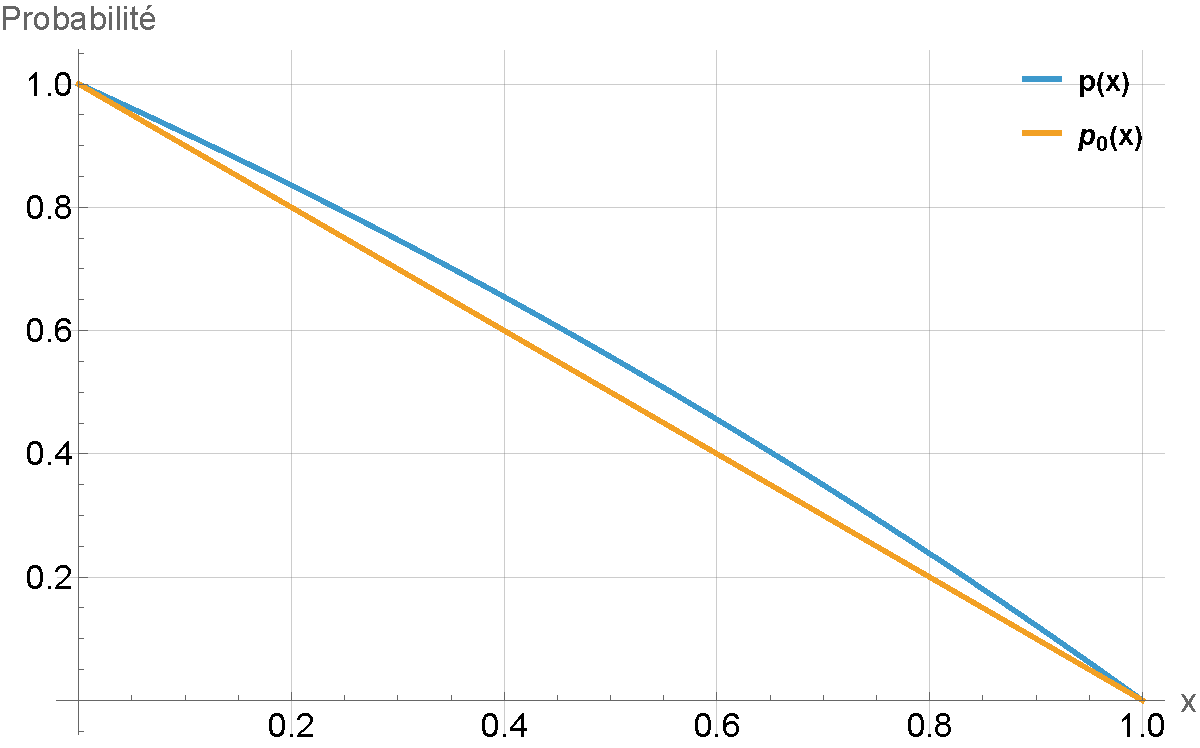
\includegraphics[width=\linewidth]{img/validation/Jumps/probability_jumps.pdf}
        \caption{Fréquence des sauts $\lambda=1$}
    \end{subfigure}
    \hfill
    \begin{subfigure}{0.45\linewidth}
        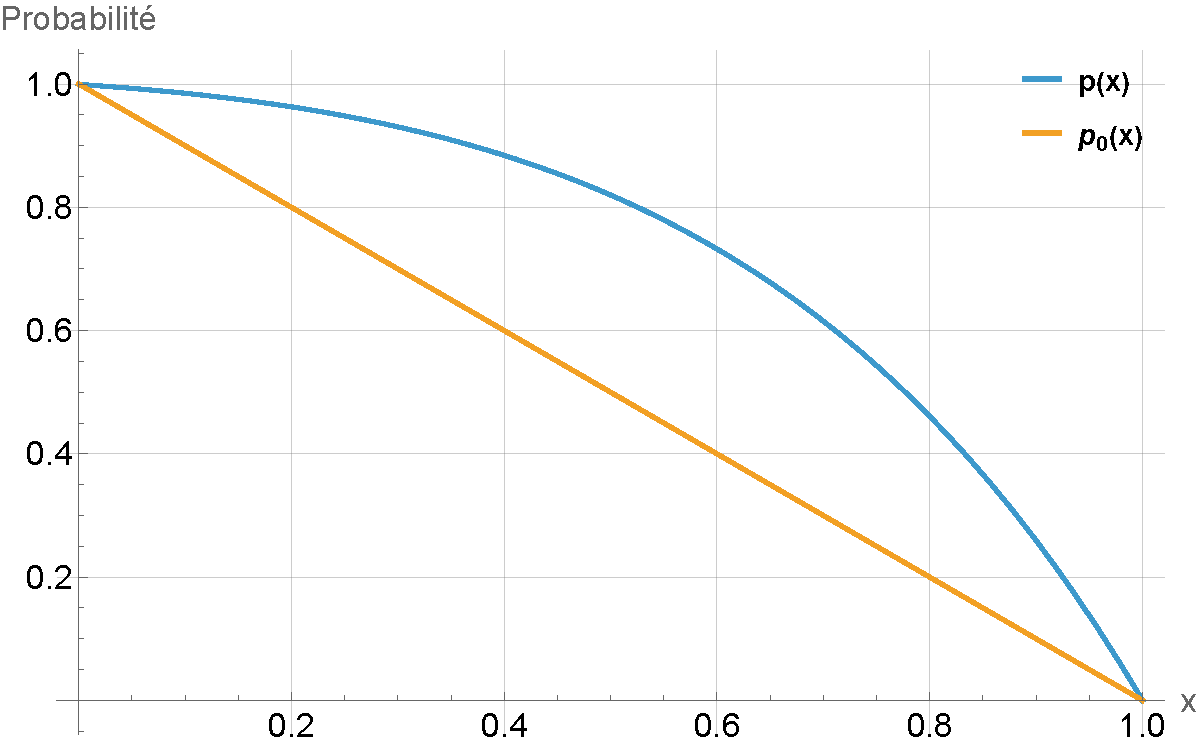
\includegraphics[width=\linewidth]{img/validation/Jumps/probability_big_jumps.pdf}
        \caption{Fréquence des sauts $\lambda=10$}
    \end{subfigure}
    \caption{Visualisation des probabilités de sortir en zéro $p(x)$ et $p_0(x)$}\label{fig:JumpsProbabilityVisualisation}
\end{figure}
\FloatBarrier\paragraph{Analyse}\mbox{}\\
Les observations suivantes peuvent être formulées:
\begin{itemize}
    \item Les conditions aux limites sont correctement satisfaites, à savoir \( p(0) = p_0(0) = 1 \) et \( p(c) = p_0(c) = 0 \);
    \item Les sauts étant négatifs, ils favorisent une sortie par la borne inférieure. La probabilité de franchissement par zéro est donc plus élevée dans le cas avec sauts ($p(x)$ en bleu);
    \item Une augmentation de la fréquence des sauts $\lambda$ entraîne une augmentation considérable de la probabilité de sortir par zéro. En effet, la multiplication des sauts tend à entraîner le processus vers la borne inférieure.
\end{itemize}
Ces résultats permettent donc de valider l'expression obtenue pour la probabilité de sortie en zéro.

\section{Fonction Dépassement Moyen \textemdash~Sauts Exponentiels Ascendants}
\subsection{Formulation générale du problème}
\paragraph{Théorème} 
\textit{Soit \(\{X(t),\,t \geq 0\}\) un processus de diffusion à sauts vérifiant les conditions d'unicité des trajectoires (\ref{trajecotry_uniqueness}), et défini par:}
\[
X(t) = X(0) + \int_0^t \mu(X(s))\,ds + \int_0^t \sigma(X(s))\,dW(s) + J(t)
\]
\textit{où \(J(t)\) est un processus de sauts pur associé à une mesure d'intensité \(\gamma(dy)\).}  

\textit{Alors, la fonction \(D(x)\) (\ref{overshoot}), représentant le dépassement moyen au-dessus de la frontière \(c\) au temps du premier passage \(\tau(x)\) (\ref{fpt_definition}), satisfait l'équation suivante:}
\begin{equation}\label{general_overshoot_ide}
    \mathcal{L}D(x) = -\int_{c - x}^{+\infty} (x + y - c)\,\gamma(dy)
\end{equation}
\textit{avec \(D(0) = D(c) = 0\) et \(\mathcal{L}\) le générateur infinitésimal du processus (voir~\ref{infinitesimal_generator}).}

\paragraph{Démonstration}
Soit $f(x)={(x-c)}_+$ la fonction mesurant un dépassement. En appliquant la formule de Dynkin (voir~\cite{dynkin1965}), il est possible d'écrire:
\begin{equation}\label{initial_dynkin}
    \mathds{E}[f(X(\tau(x)))]=f(x)+\mathds{E}\left[\int_0^{\tau(x)}\mathcal{L}f(X(s))ds\right]
\end{equation}
Pour $x\in(0,c)$:
\begin{itemize}
    \item $f(x)={(x-c)}_+=0$
    \item $f'(x)=\mathds{1}_{x\geq c}=0\implies f''(x)=0$
\end{itemize}
Le générateur infinitésimal (\ref{infinitesimal_generator}) devient:
\[
\begin{aligned}
    \mathcal{L}f(x) &= \frac{1}{2}\sigma^2(x)f''(x)+\mu(x)f'(x)+\int_{\mathds{R}}[f(x+y)-f(x)]\gamma(dy)\\
    &=\int_{\mathds{R}}(x+y-c)_+\,\gamma(dy) \\
    &=\int_{c-x}^{+\infty}(x+y-c)\gamma(dy)
\end{aligned}
\]
Le dépassement moyen est donc:
\[
D(x):=\mathds{E}\left[{(X(\tau(x))-c)}_+\right]=\mathds{E}[f(X(\tau(x)))]=\mathds{E}\left[\int_0^{\tau(x)}\left(\int_{c-x}^{+\infty}(X(s)+y-c)\gamma(dy)\right)ds\right]
\]
Alors, Abundo~\cite{abundo2013} a montré que $D(x)$ satisfait:
\[
\mathcal{L}D(x) = -\int_{c - x}^{+\infty} (x + y - c)\,\gamma(dy)
\]
avec $D(0)=D(c)=0$.\hfill$\square$

\subsection{Sauts exponentiels ascendants}
\paragraph{Lemme} 
\textit{Sous les mêmes hypothèses que précédemment, et en supposant que les sauts suivent une loi exponentielle de paramètre \(\nu > 0\) avec une intensité \(\lambda > 0\), la fonction \(D(x)\) (\ref{overshoot}) satisfait l'équation différentielle homogène d'ordre trois suivante:}
\begin{equation}\label{eq:general_ode_D}
    \begin{aligned}
        \sigma(x)^2 D'''(x)+D''(x) \left[2 \mu(x)+\sigma(x)(2\sigma'(x)-\nu  \sigma(x))\right]\\-2D'(x)[\lambda-\mu'(x)+\nu\mu(x)]=0
    \end{aligned}
\end{equation}
\textit{avec \(D(0) = D(c) = 0\).}

\paragraph{Démonstration}
Si la mesure d'intensité s'écrit:
\[
\gamma(dy):=\lambda\nu e^{-\nu y}\mathds{1}_{y\geq0}dy
\]
Alors:
\[
\int_{c-x}^{+\infty}(x+y-c)\gamma(dy)=\frac{\lambda}{\nu e^{\nu c}}e^{\nu x}
\]
L'équation (\ref{general_overshoot_ide}) devient:
\begin{equation}\label{initial_overshoot_ide}
    \frac{1}{2}\sigma^2(x)D''(x)+\mu(x)D'(x)+\lambda\int_0^\infty[D(x+y)-D(x)]\nu e^{-\nu y}dy=-\frac{\lambda}{\nu e^{\nu c}}e^{\nu x}
\end{equation}
D'abord, l'intégrale peut être simplifiée: 
\begin{equation}\label{simplified_overshoot_ide}
    \frac{1}{2}\sigma^2(x)D''(x)+\mu(x)D'(x)+\lambda\int_0^\infty D(x+y)\nu e^{-\nu y}dy-\lambda D(x)=-\frac{\lambda}{\nu e^{\nu c}}e^{\nu x}
\end{equation}
Le changement de variable $z=x+y$ donne:
\[
\begin{aligned}
    \int_0^\infty D(x+y)\nu e^{-\nu y}dy&=\int_x^\infty D(z)\nu e^{-\nu(z-x)}dz\\
    &=\nu e^{\nu x}\int_x^\infty D(z)e^{-\nu z}dz
\end{aligned}
\]
Soit:
\[
\Phi(x):=\int_x^\infty D(z)e^{-\nu z}dz
\]
L'équation (\ref{simplified_overshoot_ide}) devient:
\begin{equation}\label{ODE_Phi_D}
    \frac{1}{2}\sigma^2(x)D''(x)+\mu(x)D'(x)+\lambda\nu e^{\nu x}\Phi(x)-\lambda D(x)=-\frac{\lambda}{\nu e^{\nu c}}e^{\nu x}
\end{equation}
D'une part, la dérivée de $\Phi(x)$ est (règle de Leibniz):
\begin{equation}\label{Leibniz_rule}
    \Phi'(x)=-D(x)e^{-\nu x}\implies D(x)=-e^{\nu x }\Phi'(x)
\end{equation}
D'autre part, les dérivées de $D(x)$ s'écrivent: 
\begin{equation}\label{eq:d_derivees}
    \begin{aligned}
        D'(x) &= -\nu e^{\nu x}\Phi'(x)-e^{\nu x}\Phi''(x) \\
        D''(x)&= -\nu^2e^{\nu x}\Phi'(x)-2\nu e^{\nu x}\Phi''(x)-e^{\nu x}\Phi'''(x)
    \end{aligned}
\end{equation}
En injectant (\ref{eq:d_derivees}) dans (\ref{ODE_Phi_D}) et en éliminant les termes $-e^{\nu x}$, il découle l'\acs{EDO} d'ordre 3 suivante: 
\begin{equation}\label{general_ode_Phi}
    \begin{aligned}
        \frac{1}{2}\sigma^2(x)\Phi'''(x)+\Phi''(x)\left[\nu\sigma^2(x)+\mu(x)\right]\\+\Phi'(x)\left[\frac{1}{2}\nu^2\sigma^2(x)+\nu\mu(x)-\lambda\right]-\lambda\nu\Phi(x)=\frac{\lambda}{\nu e^{\nu c}}
    \end{aligned}
\end{equation}
Comme $D(x)$ ne dépend que de $\Phi'(x)$ (\ref{Leibniz_rule}), il est intéressant de dériver l'équation ci-dessus (\ref{general_ode_Phi}) en posant $\phi(x)=\Phi'(x)$ pour obtenir l'\acs{EDO} homogène suivante:
\begin{equation}\label{general_ode_phi}
    \begin{aligned}
        \sigma(x)^2 \phi'''(x)+2 \phi''(x) \left[\mu(x)+\sigma(x) \left(\sigma'(x)+\nu  \sigma(x)\right)\right]\\+\phi'(x) \left[-2 \lambda +2 \mu'(x)+2 \nu\mu(x)+\nu  \sigma(x) \left(4 \sigma'(x)+\nu  \sigma(x)\right)\right]\\+2 \nu  \phi(x) \left[-\lambda +\mu'(x)+\nu  \sigma(x) \sigma'(x)\right]=0
    \end{aligned}
\end{equation}
avec $D(x)=-e^{\nu x}\Phi'(x)=-e^{\nu x}\phi(x)$ et $\phi(0)=\phi(c)=0$.

Ensuite, il est possible de montrer que $\phi_1(x)=e^{-\nu x}$ est une solution particulière de (\ref{general_ode_phi}). La solution générale s'écrit donc: 
\[
\begin{aligned}
    D(x)&=-e^{\nu x}\phi(x)\\
    &=-e^{\nu x}\phi_1(x)u(x)\\
    &=-e^{\nu x}e^{-\nu x}u(x)\\
    &=-u(x)
\end{aligned}
\]
avec $u(x)$ une fonction à déterminer. En effectuant un changement de variable avec la solution particulière et en échangeant $u$ par $-D$, l'\acs{EDO} homogène d'ordre 3 suivante est obtenue: 
\[
    \begin{aligned}
        \sigma(x)^2 D'''(x)+D''(x) \left[2 \mu(x)+\sigma(x)(2\sigma'(x)-\nu  \sigma(x))\right]\\-2D'(x)[\lambda-\mu'(x)+\nu\mu(x)]=0
    \end{aligned}
\]
avec $D(0)=D(c)=0$.\hfill$\square$\\

Cette équation permet donc de résoudre le problème pour tout processus \(\{X(t),\,t\geq0\}\). Dans la suite, le \acs{CIR} avec sauts exponentiels est considéré.
\subsection{Application au CIR}
En reprenant les termes de dérive et de diffusion du \acs{CIR} (\ref{cir_eq}), l'équation (\ref{eq:general_ode_D}) devient:
\[
\sigma ^2 x D'''(x)+D''(x) \left[2 a (b-x)+\sigma ^2-\nu  \sigma ^2x\right]-2 D'(x) [a \nu  (b-x)+a+\lambda ]=0
\]
Cependant, une expression explicite pour $D(x)$, si elle existe, est très difficile à obtenir. Cela rend donc la résolution du problème général assez compliqué. 
\paragraph{Résolution exacte pour $a=0$}\phantom{}\\
En considérant le cas du \acs{CIR} à sauts sans retour à la moyenne ($a=0$) et en posant \(\sigma=c=\lambda=\nu=1\), \textit{Maple}  donne l'expression suivante:
\begin{equation}\label{overshoot_exact_sol}
    D(x)=2xe^{x}\left[\text{Ei}(x)-\text{Ei}(1)\right]
\end{equation}
avec $\text{Ei}(x)$ la fonction intégrale exponentielle (voir annexe~\ref{special_functions}).
\paragraph{Résolution approximative pour $a=0$}\phantom{}\\
En remplaçant $D(x+y)$ dans (\ref{initial_overshoot_ide}) par un développement de Taylor, il est possible de réécrire l'intégrale comme suit:
\[
\begin{aligned}
    \lambda\int_0^{+\infty}\left[D(x+y)-D(x)\right]\nu e^{-\nu y}dy&=\lambda\int_0^{+\infty}\left[\sum_{n=0}^{+\infty}\frac{y^n}{n!}\frac{d^n}{dx^n}D(x)-D(x)\right]\nu e^{-\nu y}dy\\
    &=\lambda\int_0^{+\infty}\left[\sum_{n=1}^{+\infty}\frac{y^n}{n!}\frac{d^n}{dx^n}D(x)\right]\nu e^{-\nu y}dy
\end{aligned}
\]
Ensuite, en échangeant la série et l'intégrale, le $n$-ème moment des sauts exponentiels apparaît, permettant ainsi de simplifier l'expression:
\[
\begin{aligned}
    \lambda\int_0^{+\infty}\left[\sum_{n=1}^{+\infty}\frac{y^n}{n!}\frac{d^n}{dx^n}D(x)\right]\nu e^{-\nu y}dy&=\lambda\sum_{n=0}^{+\infty}\left[\frac{1}{n!}\frac{d^n}{dx^n}D(x)\int_0^{+\infty}y^n\nu e^{-\nu y}dy\right]\\
    &=\lambda\sum_{n=0}^{+\infty}\frac{1}{n!}\frac{d^n}{dx^n}D(x)\mathds{E}\left[Y_i^n\right]\\
    &=\lambda\sum_{n=0}^{+\infty}\frac{1}{\nu^n}\frac{d^n}{dx^n}D(x)
\end{aligned}
\]
Par ailleurs, en supposant que les sauts sont petits ($\nu$ est grand), il est possible d'approximer la somme obtenue de la façon suivante:
\[
\sum_{n=0}^{+\infty}\frac{1}{\nu^n}\frac{d^n}{dx^n}D(x)\approx\frac{1}{\nu}D'(x)+\frac{1}{\nu^2}D''(x)
\]
L'équation (\ref{initial_overshoot_ide}) devient:
\begin{equation}\label{final_overshoot_ode}
    \left(\frac{1}{2}\sigma^2x+\frac{\lambda}{\nu^2}\right)D''(x)+\left[a(b-x)+\frac{\lambda}{\nu}\right]D'(x) =-\frac{\lambda}{\nu e^{\nu c}}e^{\nu x}
\end{equation}
Cette \acs{EDO} de second ordre est non homogène avec des coefficients polynomiaux et un terme exponentiel. La solution explicite, si elle existe, est difficile à obtenir. Dans la suite, un cas particulier du problème est considéré.

En éliminant le retour à la moyenne ($a=0$), l'\acs{EDO} (\ref{final_overshoot_ode}) devient:
\begin{equation}\label{particular_overshoot_ode}
    \left(\frac{1}{2}\sigma^2x+\frac{\lambda}{\nu^2}\right)D''(x)+\frac{\lambda}{\nu}D'(x) =-\frac{\lambda}{\nu e^{\nu c}}e^{\nu x}
\end{equation}
\textit{Wolfram Mathematica} donne:
\begin{equation}\label{sol_overshoot}
    \begin{aligned}
            D(x)=\frac{\lambda}{{\nu^2\sigma^2e^{\nu c}(2\lambda-\nu\sigma^2)}}\Bigg[\sigma^2\left(-C_1 \left(2 \lambda +\nu ^2 \sigma ^2 x\right)^{1-\frac{2 \lambda }{\nu  \sigma ^2}}+C_2 \nu  \left(2 \lambda -\nu  \sigma ^2\right)-2 \nu  e^{\nu  x}\right) \\-2 e^{-\frac{2 \lambda }{\nu  \sigma ^2}} \left(2 \lambda +\nu ^2 \sigma ^2 x\right) E_{1-\frac{2 \lambda }{\nu  \sigma ^2}}\left(-\frac{2 \lambda }{\nu  \sigma ^2}-x \nu \right)\Bigg]
    \end{aligned}
\end{equation}
avec $E_n(x)$ la fonction intégrale exponentielle généralisée (voir annexe~\ref{special_functions}).

\paragraph{Détermination des constantes}\phantom{}\\
Les conditions aux limites $D(0)=D(c)=0$ permettent de déterminer les deux constantes $C_1$ et $C_2$. Étant donné la longueur des expressions obtenues, celles-ci ne seront pas détaillées dans le présent document.

\subsection{Validation de l'expression obtenue}
\paragraph{Visualisation}\phantom{}\\
Afin de valider les résultat, les différentes fonctions sont tracées. D'abord, l'expression obtenue lors de la résolution exacte (\ref{overshoot_exact_sol}) est visualisée.
\begin{figure}[htb]
    \centering
    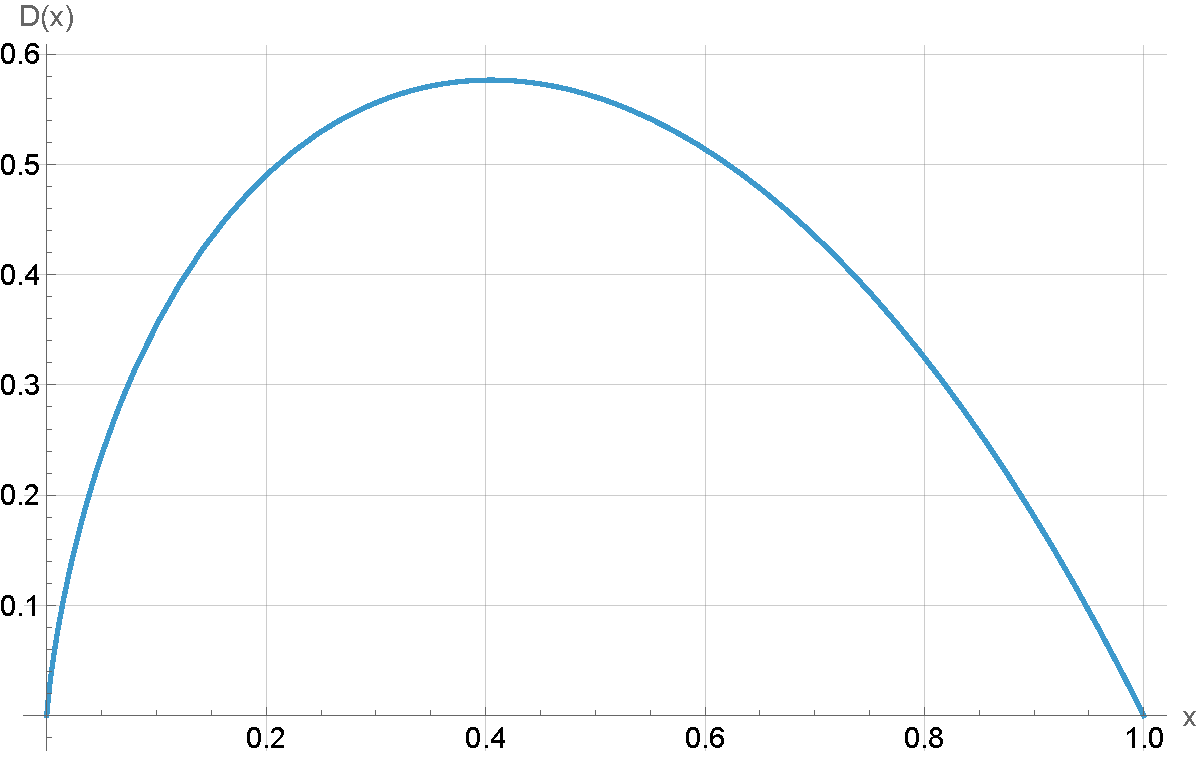
\includegraphics[width=0.5\linewidth]{img/validation/Ovs/exact.pdf}
    \caption{Visualisation de la fonction Dépassement Moyen $D(x)$}\label{fig:OvershootExactSol}
\end{figure}
\FloatBarrier Ensuite, la fonction approximative obtenue pour $D(x)$ en (\ref{sol_overshoot}) est tracée pour différentes valeurs de la fréquence des sauts $\lambda\in\{1,2,4\}$ ainsi que le paramètre de longueur des sauts $\nu\in\{10,15,20\}$.
\begin{figure}[htb]
    \centering
    \begin{subfigure}{0.45\linewidth}
        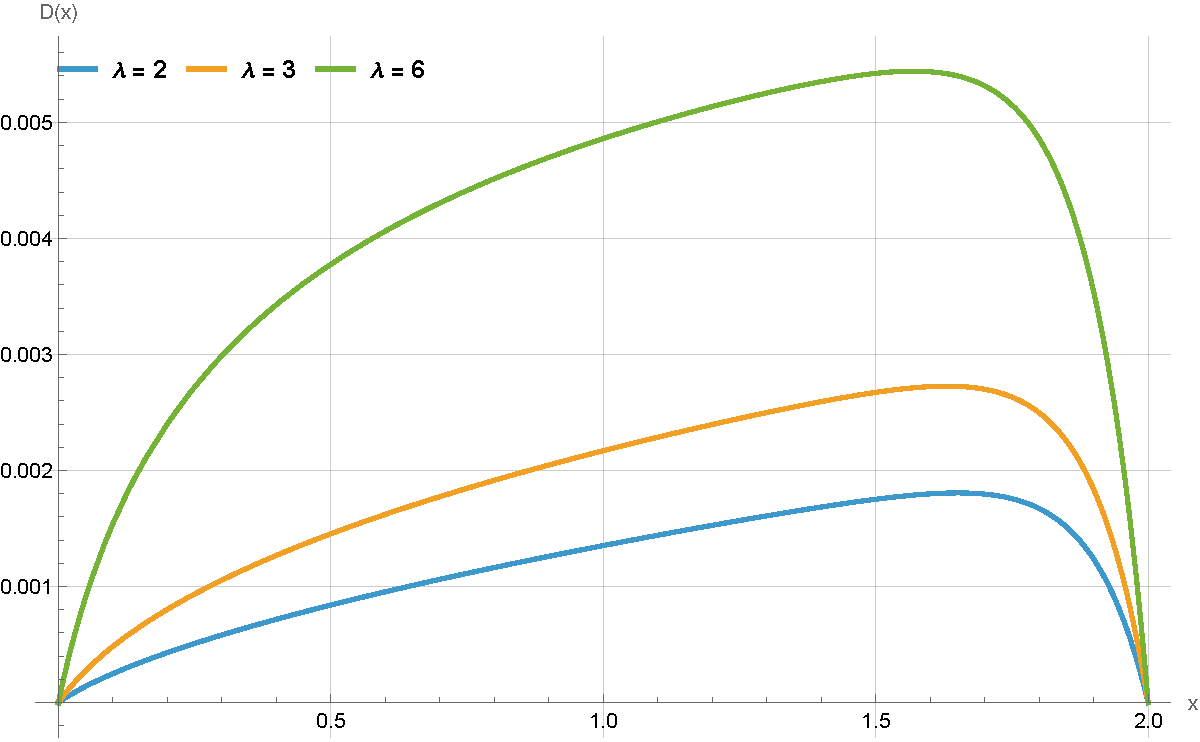
\includegraphics[width=\linewidth]{img/validation/Ovs/overshoot_lambda.pdf}
        \caption{Sensibilité de la fréquence des sauts $\lambda,\;\forall\;\lambda\in\{1,2,4\}$ \textendash~$\nu=10$}\label{fig:Overshoot_lambda_visualisation}
    \end{subfigure}
    \hfill
    \begin{subfigure}{0.45\linewidth}
        \includegraphics[width=\linewidth]{img/validation/Ovs/overshoot_nu.pdf}
        \caption{Sensibilité de la taille des sauts $\nu,\;\forall\;\nu\in\{10,15,20\}$  \textendash~$\lambda=1$}\label{fig:Overshoot_nu_visualisation}
    \end{subfigure}
    \hfill
    \caption{Visualisation de la fonction Dépassement Moyen $D(x)$}\label{fig:OvershootVisualisation}
\end{figure}
\FloatBarrier\paragraph{Analyse}\phantom{}\\
Les différents points suivants sont relevés:
\begin{itemize}
    \item Les conditions aux limites $D(0)=D(c)=0$ sont respectées;
    \item La fonction représente un \textit{dépassement moyen}, elle doit donc être positive pour toute valeur $x$ dans $[0,c]$;
    \item Une augmentation de la fréquence des sauts $\lambda$ induit une augmentation du dépassement moyen. En effet, il devient plus probable que le processus effectue un saut juste avant d'atteindre la frontière, ce qui augmente les chances de la franchir avec un certain excès;
    \item Une réduction de la taille des sauts (traduite par une augmentation de $\nu$) induit une diminution du dépassement moyen. En effet, même si un saut survient à proximité de la frontière, sa faible amplitude limite la distance franchie au-delà de celle-ci.
\end{itemize}
La fonction Dépassement Moyen $D(x)$ est donc validée.


\Chapter{COMMANDE OPTIMALE STOCHASTIQUE}\label{sec:Optimal_Control}
Ce chapitre est consacrée à l'étude du problème de commande optimale défini en (\ref{definition_optimal_control}).
\section{Formalisation du problème}
\paragraph{Dérivation de l'équation de programmation dynamique}\phantom{}\\
En reprenant la définition (\ref{value_function}) et en appliquant le principe d'optimalité de Bellman, il découle:
\begin{equation}\label{Bellman_optimality}
        F(x) = \inf_u\mathds{E}\left[\int_0^{\delta t}\left(\frac{1}{2}q\left[X_u(s)\right]u^2\left[X_u(s)\right]+r\left[X_u(s)\right]\right)ds+F(X_u(\delta t))\right]
\end{equation}
D'une part, pour $\delta t$ petit, il est possible d'écrire:
\begin{equation}\label{cost_function_simplification}
    \int_0^{\delta t}\left(\frac{1}{2}q\left[X_u(s)\right]u^2\left[X_u(s)\right]+r\left[X_u(s)\right]\right)ds=\left(\frac{1}{2}q(x){u(x)}^2+r(x)\right)\delta t+o(\delta t)
\end{equation}
D'autre part, un développement de Taylor combiné avec la formule d'Itô~\cite{ito1944} (appliquée au processus contrôlé de dynamique (\ref{controlled_process})) permet d'écrire (en supposant que $F\in C^2$):
\begin{equation}\label{taylor_ito}
    \begin{aligned}
        \mathds{E}[F(X_u(\delta t))]&=F(x)+\mathds{E}[dF(X_u(\delta t))]+o(\delta t)\\
        &=F(x)+\mathds{E}\left[F'(X_u(\delta t))dX_u(t)+\frac{1}{2}F''(X_u(\delta t))d{\langle X_u\rangle}_{\delta t} \right]+o(\delta t)\\
        &=F(x)+\left[a(b-x)+b(x)u(x)\right]F'(x)\delta t+\frac{1}{2}\sigma^2xF''(x)\delta t+o(\delta t)
    \end{aligned}
\end{equation}
où \({\langle X_u\rangle}_t\) dénote la variation quadratique du processus \(X_u(t)\).

En injectant (\ref{cost_function_simplification}) et (\ref{taylor_ito}) dans (\ref{Bellman_optimality}), il découle:
\begin{equation}\label{initial_minimisation problem}
    \begin{aligned}
        F(x)&=\inf_u\Bigg\{\left(\frac{1}{2}q(x){u(x)}^2+r(x)\right)\delta t+F(x)+\left[a(b-x)+b(x)u(x)\right]F'(x)\delta t\\&\quad\quad\quad\quad\quad\quad\quad\quad\quad\quad\quad\quad\quad\quad\quad\quad\quad\quad\quad\quad+\frac{1}{2}\sigma^2xF''(x)\delta t+o(\delta t)\Bigg\}
    \end{aligned}
\end{equation}
Ensuite, en retranchant $F(x)$ des deux côtés, en divisant partout par $\delta t$ et en prenant la limite lorsque $\delta t\to0$, l'équation de programmation dynamique est obtenue:
\begin{equation}\label{minimisation_problem}
    0=\min_u\left\{r(x)+\frac{1}{2}q(x)u^2(x)+[a(b-x)+b(x)u(x)]F'(x)+\frac{1}{2}\sigma^2xF''(x)\right\}
\end{equation}
\paragraph{Détermination de la commande optimale et dérivation de l'équation associée}\phantom{}\\
La minimisation à faire dans (\ref{minimisation_problem}) est en fonction de $u(x)$. Le terme à minimiser est:
\[
f(u(x))=\frac{1}{2}q(x){u(x)}^2+b(x)u(x)F'(x)
\]
La minimisation donne:
\begin{equation}\label{optimal_control}
    \begin{aligned}
        f'(u^*(x))&=0\\
        q(x)u^*(x)+b(x)F'(x)&=0\\
    u^*(x)&=-\frac{b(x)}{q(x)}F'(x)
    \end{aligned}
\end{equation}
Par ailleurs, la dérivée seconde est: 
\[
f''(u(x))=q(x)\quad\forall\;u(x)
\]
Puisque \( q(x) > 0 \) par hypothèse (\ref{definition_optimal_control}), la dérivée seconde par rapport au contrôle est strictement positive. L'expression de \( u^*(x) \) obtenue en (\ref{optimal_control}) réalise donc bien un minimum global. Il s'agit ainsi du contrôle optimal.

En injectant ce dernier (\ref{optimal_control}) dans (\ref{minimisation_problem}), l'équation \acl{HJB} est obtenue, régissant la fonction valeur associée à la commande optimale:
\begin{equation}\label{control_equation}
    r(x) - \frac{{b(x)}^2}{2q(x)}{\left[F'(x)\right]}^2 + a(b - x)F'(x) + \frac{1}{2}\sigma^2 x F''(x) = 0
\end{equation}
avec $F(0)=F(c)=0$ et $r(x)\neq0, b(x)\neq0, q(x)>0$.


\section{Résolution du problème sous différentes configurations}
\subsection{P1 \textemdash~Résolution}\label{p1}
\paragraph{Résolution du problème}\phantom{}\\
Il faut donc procéder à la résolution de l'équation (\ref{control_equation}). Whittle~\cite{whittle1982} a montré que la transformation: 
\[F(x)=-K\log(\varphi(x))\]
avec $\varphi(0)=\varphi(c)=1$ permet de linéariser l'équation si:
\[
K{b(x)}^2=\sigma^2xq(x),\quad K\in\mathds{R}
\]
L'équation devient:
\begin{equation}\label{linearised_equation}
    \frac{1}{2}\sigma^2 x\varphi''(x) + a(b - x)\varphi'(x) - \frac{r(x)}{K}\varphi(x) = 0
\end{equation}
Dans le cas où le terme suivant est constant:
\begin{equation}\label{condition}
    \frac{r(x)}{K}\equiv k\in\mathds{R}\;\forall\;x
\end{equation}
l'équation (\ref{linearised_equation}) est identique à celle de la \acl{FGM} $M(x;\alpha)$ pour:
\[
\alpha\equiv\frac{r(x)}{K}
\]
Cela permet de résoudre une multitude de problèmes en supposant différentes formes pour $r(x)$, $b(x)$ et $q(x)$ tout en satisfaisant la condition (\ref{condition}). 

Soit les coûts suivants:
\begin{itemize}
    \item $r(x) = \rho$: coût immédiat constant, indépendant de l'état $x$ et du contrôle;
    \item $b(x) = \beta x$: coût du contrôle proportionnel à $x$ sur la dynamique;
    \item $q(x) = \kappa x$: poids pénalisant l'intensité du contrôle, linéaire avec $x$.
\end{itemize}

Cela donne:
\[
K\equiv\frac{\kappa \sigma^2}{\beta^2}
\]
L'équation devient:
\begin{equation}\label{eq_exemple1}
    \frac{1}{2}\sigma^2 x\varphi''(x) + a(b - x)\varphi'(x) - \frac{\rho\beta^2}{\kappa \sigma^2}\varphi(x) = 0
\end{equation}
La solution est:
\[
\varphi(x)=C_1\Phi\left(\frac{\rho\beta^2}{a\kappa \sigma^2},\frac{2ab}{\sigma^2},\frac{2ax}{\sigma^2}\right) + C_2\Psi\left(\frac{\rho\beta^2}{a\kappa \sigma^2},\frac{2ab}{\sigma^2},\frac{2ax}{\sigma^2}\right)
\]
Les conditions aux limites $\varphi(0)=\varphi(1)=1$ permettent de déterminer les constantes $C_1$ et $C_2$:
\begin{equation}\label{control_constants}
    \begin{aligned}
        C_1=\frac{\Psi\left(\frac{\beta ^2 \rho }{a \kappa  \sigma ^2},\frac{2 a b}{\sigma ^2},0\right)-\Psi\left(\frac{\beta ^2 \rho }{a \kappa  \sigma ^2},\frac{2 a b}{\sigma ^2},\frac{2 a c}{\sigma ^2}\right)}{\Psi\left(\frac{\beta ^2 \rho }{a \kappa  \sigma ^2},\frac{2 a b}{\sigma ^2},0\right) \, \Phi\left(\frac{\beta ^2 \rho }{a \kappa  \sigma ^2};\frac{2 a b}{\sigma ^2};\frac{2 a c}{\sigma ^2}\right)-\Psi\left(\frac{\beta ^2 \rho }{a \kappa  \sigma ^2},\frac{2 a b}{\sigma ^2},\frac{2 a c}{\sigma ^2}\right)} \\
        C_2= \frac{\, \Phi\left(\frac{\beta ^2 \rho }{a \kappa  \sigma ^2};\frac{2 a b}{\sigma ^2};\frac{2 a c}{\sigma ^2}\right)-1}{\Psi\left(\frac{\beta ^2 \rho }{a \kappa  \sigma ^2},\frac{2 a b}{\sigma ^2},0\right) \, \Phi\left(\frac{\beta ^2 \rho }{a \kappa  \sigma ^2};\frac{2 a b}{\sigma ^2};\frac{2 a c}{\sigma ^2}\right)-\Psi\left(\frac{\beta ^2 \rho }{a \kappa  \sigma ^2},\frac{2 a b}{\sigma ^2},\frac{2 a c}{\sigma ^2}\right)}
    \end{aligned}
\end{equation}
L'expression analytique de la fonction valeur est donc:
\begin{equation}\label{sol_control_1}
    F(x)=-\frac{\kappa \sigma^2}{\beta^2} \log\left[C_1\Phi\left(\frac{\rho\beta^2}{a\kappa \sigma^2},\frac{2ab}{\sigma^2},\frac{2ax}{\sigma^2}\right) + C_2\Psi\left(\frac{\rho\beta^2}{a\kappa \sigma^2},\frac{2ab}{\sigma^2},\frac{2ax}{\sigma^2}\right)\right]
\end{equation}
Par ailleurs, le contrôle optimal est
\begin{equation}\label{optimal_control_1}
    u^*(x)=-\frac{\beta}{\kappa}F'(x)
\end{equation}

\subsection{P1 \textemdash~Visualisation}
La fonction valeur $F(x)$ (\ref{sol_control_1},~\ref{control_constants}) et le contrôle optimal (\ref{optimal_control_1}) sont tracés. D'abord, tous les paramètres des coûts sont fixés: $\rho=\beta=\kappa=1$.
\begin{figure}[htb]
    \centering
    \begin{subfigure}{0.45\linewidth}
        \includegraphics[width=\linewidth]{img/validation/P1/p1_value.pdf}
        \caption{P1 \textemdash~Fonction Valeur $F(x)$}\label{fig:ValueVisualisation1}
    \end{subfigure}
    \hfill
    \begin{subfigure}{0.45\linewidth}
        \includegraphics[width=\linewidth]{img/validation/P1/p1_control.pdf}
        \caption{P1 \textemdash~Contrôle Optimal $u^*(x)$}\label{fig:ControlVisualisation1}
    \end{subfigure}
    \caption{P1 \textemdash~Visualisation de la fonction valeur et du contrôle optimal}\label{fig:ValueControlComparison1}
\end{figure}\FloatBarrier De plus, il est intéressant d'analyser la sensibilité de ces fonctions par rapport à la variation des coûts. Les différentes valeurs des paramètres suivants sont évaluées:
\begin{itemize}
    \item Paramètre du coût immédiat $\rho,\;\forall\;\rho\in\{1,2,3,4\}$;
    \item Paramètre du coût de contrôle $\beta,\;\forall\;\beta\in\{1,2,3,4\}$;
    \item Paramètre du poids pénalisant l'intensité du contrôle $\kappa,\;\forall\;\kappa\in\{1,2,3,4\}$.
\end{itemize}
\begin{figure}[htb]
    \centering
    % Ligne 1 : Sensibilité à rho
    \begin{subfigure}{0.49\linewidth}
        \includegraphics[width=\linewidth]{img/validation/P1/p1_R_value.pdf}
        \caption{P1 \textemdash~Fonction Valeur $F(x)$, $r(x)=\rho$}\label{fig:RhoValueVisualisation1}
    \end{subfigure}
    \hfill
    \begin{subfigure}{0.49\linewidth}
        \includegraphics[width=\linewidth]{img/validation/P1/p1_R_control.pdf}
        \caption{P1 \textemdash~Contrôle Optimal $u^*(x)$, $r(x)=\rho$}\label{fig:RhoControlVisualisation1}
    \end{subfigure}

    % Ligne 2 : Sensibilité à beta
    \begin{subfigure}{0.49\linewidth}
        \includegraphics[width=\linewidth]{img/validation/P1/p1_B_value.pdf}
        \caption{P1 \textemdash~Fonction Valeur $F(x)$, $b(x)=\beta x$}\label{fig:BetaValueVisualisation1}
    \end{subfigure}
    \hfill
    \begin{subfigure}{0.49\linewidth}
        \includegraphics[width=\linewidth]{img/validation/P1/p1_B_control.pdf}
        \caption{P1 \textemdash~Contrôle Optimal $u^*(x)$, $b(x)=\beta x$}\label{fig:BetaControlVisualisation1}
    \end{subfigure}

    % Ligne 3 : Sensibilité à kappa
    \begin{subfigure}{0.49\linewidth}
        \includegraphics[width=\linewidth]{img/validation/P1/p1_K_value.pdf}
        \caption{P1 \textemdash~Fonction Valeur $F(x)$, $q(x)=\kappa x$}\label{fig:KappaValueVisualisation1}
    \end{subfigure}
    \hfill
    \begin{subfigure}{0.49\linewidth}
        \includegraphics[width=\linewidth]{img/validation/P1/p1_K_control.pdf}
        \caption{P1 \textemdash~Contrôle Optimal $u^*(x)$, $q(x)=\kappa x$}\label{fig:KappaControlVisualisation1}
    \end{subfigure}
    \caption{P1 \textemdash~Sensibilité des fonctions valeur $F(x)$ et contrôle optimal $u^*(x)$}\label{fig:ParamSensitivityP1}
\end{figure}
\FloatBarrier Par ailleurs, une simulation d'une trajectoire contrôlée et d'une trajectoire non contrôlée est effectuée en utilisant un même tirage aléatoire, afin de permettre une comparaison pertinente entre les deux dynamiques.
\begin{figure}[htb]
    \centering
    \includegraphics[width=0.9\linewidth]{img/validation/P1/p1_control_simulation.pdf}
    \caption{P1 \textemdash~Visualisation de l'effet de la commande optimale}\label{fig:Simulation1}
\end{figure}\FloatBarrier\subsection{P2 \textemdash~Résolution}\label{p3}
Soit le problème suivant:
\begin{itemize}
    \item $r(x) = x^2$: coût immédiat quadratique en $x$, indépendant du contrôle;
    \item $b(x) = x$: coût du contrôle linéaire égal à $x$;
    \item $q(x) \equiv 1$: poids pénalisant l'intensité du contrôle constant.
\end{itemize}
La condition (\ref{condition}) n'étant pas satisfaite, ce problème ne permet pas une linéarisation facile. Il faut donc le résoudre d'une autre manière. En éliminant le retour à la moyenne ($a=0$) et en posant $\sigma=1$, l'équation (\ref{control_equation}) se réduit à:
\begin{equation}\label{reduced_control_equation}
    x^2-\frac{x^2}{2}{F'(x)}^2+\frac{1}{2}xF''(x)=0
\end{equation}
Le logiciel de calcul symbolique \textit{Maple} donne comme solution pour $F(0)=0$ (avec $C_1$ une constante à déterminer):
\[
    F(x)=\int_0^x-\sqrt{2}\tanh\left(\frac{\sqrt{2}z^2}{2}+C_1\sqrt{2}\right)dz
\]
En posant $c=1$, la valeur de $C_1$ qui satisfait $F(c)=F(1)=0$ est $C_1\simeq -0.1652$. Donc, la forme finale de la fonction valeur est obtenue:
\begin{equation}\label{sol_control_3}
    F(x)\simeq \int_0^x-\sqrt{2}\tanh\left(\frac{\sqrt{2}z^2}{2}-0.1652\sqrt{2}\right)dz
\end{equation}
La commande optimale est donc:
\begin{equation}\label{optimal_control_3}
    u^*(x)\simeq x\sqrt{2}\tanh\left(\frac{\sqrt{2}x^2}{2}-0.1652\sqrt{2}\right)
\end{equation}
\subsection{P2 \textemdash~Visualisation}
La fonction valeur (\ref{sol_control_3}) ainsi que la commande optimale (\ref{optimal_control_3}) sont tracés.
\begin{figure}[htb]
    \centering
    \begin{subfigure}{0.45\linewidth}
        \includegraphics[width=\linewidth]{img/validation/P3/p3_value.pdf}
        \caption{P2 \textemdash~Fonction Valeur $F(x)$}\label{fig:ValueVisualisation3}
    \end{subfigure}
    \hfill
    \begin{subfigure}{0.45\linewidth}
        \includegraphics[width=\linewidth]{img/validation/P3/p3_control.pdf}
        \caption{P2 \textemdash~Contrôle Optimal $u^*(x)$}\label{fig:ControlVisualisation3}
    \end{subfigure}
    \caption{P2 \textemdash~Visualisation de la fonction valeur et du contrôle optimal}\label{fig:ValueControlComparison3}
\end{figure}
\FloatBarrier Enfin, une simulation est aussi effectuée. 
\begin{figure}[htb]
    \centering
    \includegraphics[width=0.9\linewidth]{img/validation/P3/p3_control_simulation.pdf}
    \caption{P2 \textemdash~Visualisation de l'effet de la commande optimale}\label{fig:Simulation3}
\end{figure}\FloatBarrier\section{Validation}
Il est important de souligner que, dans les deux problèmes étudiés et pour les différentes valeurs des paramètres considérés:
\begin{itemize}
    \item Les conditions aux limites $F(0)=F(c)=0$ sont toujours respectées;
    \item La fonction valeur est toujours positive, le coût encouru étant nécessairement positif;
    \item Le contrôle optimal est négatif lorsque \( x \to 0^+ \), l'optimiseur cherchant à diriger rapidement le processus vers la frontière inférieure, plus proche. Inversement, pour \( x \to c^-\), le contrôle devient positif afin d'accélérer l'atteinte de la frontière supérieure;
    \begin{sloppypar}\item Une augmentation du coût immédiat $\rho$, induisant une hausse du coût encouru (\ref{fig:RhoValueVisualisation1}), entraîne un renforcement du contrôle optimal ($|u^*(x)|$ augmente dans~\ref{fig:RhoControlVisualisation1}), traduisant ainsi une volonté accrue de quitter l'intervalle aussi rapidement que possible;\end{sloppypar}
    \item Une hausse du coût du contrôle $\beta$ incite à intensifier le contrôle optimal (\ref{fig:BetaControlVisualisation1}) afin de quitter l'intervalle plus rapidement. Cette stratégie réduit la durée d'exposition au coût instantané, ce qui compense partiellement le surcoût du contrôle et diminue le coût total encouru $F(x)$ (\ref{fig:BetaValueVisualisation1});
    \item Une augmentation du poids pénalisant le contrôle $\kappa$, induisant une hausse du coût encouru (\ref{fig:KappaValueVisualisation1}), entraîne une relaxation du contrôle optimal (\ref{fig:KappaControlVisualisation1}). En effet, plus le poids du contrôle est élevé, moins il est intéressant d'appliquer un contrôle fort;
    \item Les simulations (\ref{fig:Simulation1},~\ref{fig:Simulation3}) mettent en évidence l'effet du contrôle optimal, qui accélère la sortie du processus par rapport au cas non contrôlé. Pour valider cette observation, 1000 trajectoires sont simulées pour chaque problème, et la durée moyenne jusqu'à la sortie est comparée. Un facteur d'accélération est ensuite estimé (voir annexe~\ref{control_simulations} pour les détails du calcul):
    \begin{table}[htb]
        \centering
        \caption{Accélérations moyennes du temps de sortie}\label{tab:acceleration_results}
        \renewcommand{\arraystretch}{1.1}
        \begin{tabular}{||c|c||}
        \hline
        Problème & Accélération Moyenne \\\hline\hline
        P1 & 2.660552 \\
        %P2 & 2.690582 \\
        P2 & 1.065163 \\\hline
        \end{tabular}
    \end{table}
\end{itemize}\FloatBarrier Ainsi, les expressions obtenues pour la fonction valeur $F(x)$ et le contrôle optimal $u^*(x)$ sont validées.

Ces observations générales fournissent un cadre d'interprétation cohérent pour les stratégies optimales. Ces dernières sont détaillées dans la partie qui suit.
\section{Politiques Optimales}
À partir des simulations réalisées, de l'analyse des profils des commandes optimales \( u^*(x) \) illustrés dans les figures~\ref{fig:ControlVisualisation1} et~\ref{fig:ControlVisualisation3}, ainsi que de leur mise en relation avec les structures de coûts propres à chaque configuration, il est possible de caractériser précisément les différentes stratégies de contrôle optimales associées à chacun des problèmes étudiés:
\begin{itemize}
    \item \textbf{Stratégie P1}: La politique optimale en configuration P1 adopte une structure à seuil, avec un point critique situé autour de \(x^* \approx 0.33\). Pour \(x < x^*\), le contrôle diverge rapidement vers \(-\infty\), tirant agressivement le processus vers la borne inférieure. Ce comportement traduit une exploitation stratégique de la structure des coûts \(b(x) = q(x) = x\), qui tendent eux aussi vers zéro, rendant le contrôle intensif peu pénalisant dans cette région. Inversement, pour \(x > x^*\), le contrôle devient positif mais reste modéré, poussant le processus vers la borne supérieure de l'intervalle jusqu'à \(u(1)\approx1.4\).

    L'asymétrie du seuil observée dans cette politique s'explique par la nature du coût d'état constant \(r(x)\equiv1\) ainsi que deux mécanismes complémentaires. Premièrement, la dynamique du processus \acs{CIR} possède un terme de retour à la moyenne dirigé vers \(b\) (fixé ici à 0.9). Ainsi, dès que le processus est situé en dessous de cette valeur, il bénéficie naturellement d'une poussée ascendante, ce qui rend avantageux de renforcer cette tendance au-delà du seuil \(x^*\) par un contrôle positif. Deuxièmement, la diffusion du processus étant proportionnelle à \(\sqrt{X(t)}\), les perturbations aléatoires sont fortement atténuées près de zéro. Il est donc inefficace de chercher à atteindre la borne inférieure depuis une position trop éloignée, et le contrôle n'est justifié dans cette direction que pour des valeurs suffisamment petites de \(x\) (en-dessous du seuil $x^*$). Ce comportement est corroboré par une analyse empirique: sur 1000 trajectoires simulées, le processus s'échappe par la borne supérieure dans 67\,\% des cas (voir~\ref{tab:simulation_exit_frequency});
    \item \textbf{Stratégie P2}: La politique optimale correspond à une stratégie d'évasion passive. Bien qu'un seuil \(x^*\approx0.574\) subsiste, marquant l'inversion du signe de la commande, l'amplitude de \(u(x)\) demeure globalement faible. En effet, avec un poids pénalisant l'intensité du contrôle constant \(q(x) \equiv 1\), l'optimiseur n'est pas particulièrement incité à appliquer une commande intensive. Celui-ci n'intervient donc qu'avec un contrôle faible, sans chercher à forcer activement la dynamique du processus. Ce comportement est confirmé par le faible facteur d'accélération observé, estimé à 1.06 (voir~\ref{tab:acceleration_results}), ainsi qu'une fréquence de sortie pour chaque frontière presque identique à celle du processus non-contrôlé (\ref{tab:simulation_exit_frequency}), indiquant une quasi-absence de différence entre les trajectoires contrôlées et non contrôlées.
\end{itemize}

\Chapter{CONCLUSION}\label{sec:Conclusion}
\section{Synthèse des travaux}

Ce mémoire s'inscrit dans le cadre de l'étude des temps de premier passage et des problèmes de commande optimale appliqués au processus \acs{CIR}, à la fois en diffusion pure et en présence de sauts. L'objectif principal consistait à obtenir, sous forme analytique, plusieurs fonctions d'intérêt: la fonction génératrice des moments du temps de sortie, la fonction temps moyen de sortie, l'aire moyenne sous la trajectoire, la probabilité de sortie en zéro, la fonction de dépassement moyen dans le cas avec sauts et la fonction valeur des problèmes de commande optimale considérés ainsi que le contrôle optimal associé.

Ces résultats ont été obtenus en résolvant des équations différentielles ordinaires faisant intervenir la dynamique du processus. Les méthodes utilisées incluent notamment des changements de variables adaptés (comme la transformation de Kummer), l'usage de fonctions spéciales (fonctions hypergéométriques, fonctions Gamma, fonction Intégrale Exponentielle), ainsi que le recours à des outils de calcul symbolique comme \textit{Wolfram Mathematica} ou encore \textit{Maple}.

L'analyse des résultats a permis de valider les expressions obtenues à l'aide des conditions aux limites et des propriétés structurelles attendues des solutions. Les visualisations produites viennent renforcer cette validation en illustrant les comportements théoriques anticipés.

Enfin, l'étude des problèmes de commande optimale associés au processus \acs{CIR} a permis de déterminer les fonctions valeur et les stratégies optimales dans quatre configurations de coûts différentes. Les solutions proposées satisfont les conditions de régularité et de positivité attendues, confirmant ainsi la solidité des approches analytiques adoptées. De plus, les simulations effectuées mettent en avant l'effet des différentes commandes optimales trouvées, permettant ainsi de valider davantage les expressions obtenues.

Les résultats relatifs à la fonction génératrice des moments, à l'aire moyenne, au temps moyen de sortie (avec et sans sauts), à la probabilité de sortie en zéro (avec et sans sauts), ainsi qu'au problème de contrôle non linéarisable P3, exposés dans ce mémoire, ont fait l'objet d'un article de recherche publié dans la revue internationale \textit{WSEAS Transactions on Mathematics}~\cite{lefebvre2025}.

\section{Limitations}

Les résultats présentés dans ce mémoire reposent sur des hypothèses spécifiques concernant les paramètres du processus CIR et la structure des coûts dans les problèmes de commande optimale. En particulier, les paramètres \(a\), \(b\) et \(\sigma\) du processus \acs{CIR} sont supposés constants dans le cadre de cette étude. Cette hypothèse permet de simplifier les équations différentielles associées, mais elle peut s'avérer restrictive lorsque ces paramètres varient en fonction du temps ou de l'état du processus. De plus, bien que les solutions analytiques proposées soient valides dans ces contextes particuliers, comme le \acs{CIR} sans retour à la moyenne, elles peuvent perdre en pertinence lorsque la dérive est non-négligeable. Par ailleurs, les configurations de coûts étudiées en commande optimale réduisent le problème général à des cas spécifiques. Dans le cas où les coûts sont plus complexes, obtenir des formes fermées pour les solutions devient presque impossible.

\section{Perspectives et améliorations futures}

Afin de surmonter les limitations identifiées, plusieurs pistes de recherche peuvent être explorées. Une première perspective consisterait à étendre l'étude au processus de Chen~\cite{chen1996} dans lequel la volatilité et la moyenne long-terme du processus sont stochastiques. D'autres extensions du \acs{CIR} à étudier seraient celles qui permettent au processus de prend des valeurs négatives comme le CIR\#~\cite{orlando2019}, le CIR- et le CIR-{}-~(voir~\cite{difrancesco2021} et~\cite{difrancesco2022}).

Une deuxième piste pourrait consister à explorer des méthodes numériques permettant de compléter les résultats analytiques dans des situations où les solutions exactes ne sont pas accessibles. L'utilisation de techniques de simulation Monte Carlo comme lors de l'étude du dépassement moyen (\ref{fig:OvershootSimulationLambda}) ou de méthodes numériques pour la résolution des équations de \acs{HJB} pourrait permettre de mieux appréhender les comportements dans des cadres plus réalistes.

Enfin, l'extension des modèles de commande optimale pour inclure des coûts non linéaires ou des contraintes supplémentaires pourrait offrir de nouvelles perspectives, en particulier dans le cadre de la gestion de portefeuille ou de la couverture d'actifs financiers sous contraintes réglementaires. Cependant, la complexité des équations associées augmentera considérablement.

En conclusion, ce mémoire propose une approche analytique rigoureuse pour l'étude des problèmes de premier passage et de commande optimale appliqués au processus \acs{CIR}. Les résultats obtenus constituent une base solide pour des développements futurs dans des contextes plus généraux ou appliqués.         % Conclusion.
%\backmatter
\ifthenelse{\equal{\Langue}{english}}{
	\renewcommand\bibname{REFERENCES}
	\bibliography{Document}
	\bibliographystyle{IEEEtran}			% Style bibliographique / Bibliography style 
}{
	\renewcommand\bibname{RÉFÉRENCES}
	\bibliography{Document}
	\bibliographystyle{IEEEtran-francais}    % Style bibliographique / Bibliography style 
}
%
\ifthenelse{\equal{\AnnexesPresentes}{O}}{
	\appendix%
	\newcommand{\Annexe}[1]{\annexe{#1}\setcounter{figure}{0}\setcounter{table}{0}\setcounter{footnote}{0}}%
	%%
%%  Annexes
%%
%%  Note: Ne pas modifier la ligne ci-dessous. / Do not modify the following line.
\phantomsection
\ifthenelse{\equal{\Langue}{english}}{
	\addcontentsline{toc}{compteur}{APPENDICES}
}{
	\addcontentsline{toc}{compteur}{ANNEXES}
}
%%
%%
%%  Toutes les annexes doivent être inclues dans ce document
%%  les unes à la suite des autres.
%%  All annexes must be included in this document one after the other.



\Annexe{Fonctions Spéciales}\label{special_functions}
Cette annexe contient une définition de toutes les fonctions spéciales utilisées dans ce mémoire. Pour plus d'information, voir~\cite{NIST:DLMF}.
\section*{Fonctions Gamma}
\begin{itemize}
    \item La fonction Gamma est définie par:
    \[
        \begin{aligned}
            \Gamma(z)&:=\int_0^{+\infty}t^{z-1}e^{-t}dt \\
            \Gamma(n)&:=(n-1)!
        \end{aligned}
    \]
    Elle permet de généraliser la notion de factoriel:
    \[
    \forall\;z\in\mathds{R}\setminus\mathds{Z}^-,\Gamma(z+1)=z\Gamma(z)
    \]
    \item Les fonction Gamma incomplètes sont définies par:
    \[
    \begin{aligned}
        \Gamma(s,x)&:=\int_x^{+\infty}t^{s-1}e^{-t}dt \\
        \gamma(s,x)&:=\int_0^x t^{s-1}e^{-t}dt
    \end{aligned}
    \] 
\end{itemize}
\section*{Symbole de Pochhammer}
Le symbole de Pochhammer (ou factoriel ascendant) est défini par:
\[
{(a)}_n:=\prod_{i=1}^n (a+i-1)
\]
\section*{Fonctions hypergéométriques}
\begin{itemize}
    \item Les fonctions hypergéométriques confluentes de première et seconde espèce (aussi appelées fonctions de Kummer et Tricomi) sont définies par:
    \[
        \begin{aligned}
            \Phi(s, t, z) &:= \sum_{n=0}^{\infty} \frac{{(s)}_n \, z^n}{{(t)}_n \, n!}  \\
            \Psi(s,t,z) &:= \frac{\Gamma(1-t)}{\Gamma(s+1-t)}\Phi(s,t,z)+\frac{\Gamma(t-1)}{\Gamma(s)}z^{1-t}\Phi(s+1-t,2-t,z)
        \end{aligned}
    \]
    \item La fonction hypergéométrique généralisée est définie par:
    \[
    _p F_q\left(\begin{bmatrix}s_1\\\vdots\\s_p\end{bmatrix},\begin{bmatrix}t_1\\\vdots\\t_q\end{bmatrix},\,z\right):=\sum_{n=0}^\infty\frac{{(s_1)}_n\cdots{(s_p)}_n}{{(t_1)}_n\cdots {(t_q)}_n}\frac{z^n}{n!}
    \]
    Il est intéressant de noter que la fonction hypergéométrique confluente de première espèce $\Phi(\cdot,\cdot,\cdot)$ n'est autre que le cas particulier $_1F_1(\cdot,\cdot,\cdot)$.
\end{itemize}
\section*{Fonctions intégrale exponentielle}
\begin{itemize}
    \item La fonction intégrale exponentielle est définie par:
    \[
    \text{Ei}(x):=-\int^{\infty}_{-x}\frac{e^{-t}}{t}dt
    \]
    \item La fonction intégrale exponentielle généralisée est définie par:
    \[
    E_n(x):=\int_1^{+\infty}\frac{e^{xt}}{t^n}dt
    \]
    Il est intéressant de noter que, pour $x>0$:
    \[\text{Ei}(x)=-E_1(-x)\]
\end{itemize}
\section*{Fonctions de Bessel}
\begin{itemize}
    \item Les fonctions de Bessel de première et seconde espèce sont définies par:
    \[
    \begin{aligned}
        J_\alpha(x)&:=\sum_{m=0}^{+\infty}\frac{(-1)^m}{m!\Gamma(m+\alpha+1)}{\left(\frac{x}{2}\right)}^{2m+\alpha} \\
        Y_\alpha(x)&:=\frac{J_\alpha(x)\cos(\alpha\pi)-J_{-\alpha}(x)}{\sin(\alpha\pi)}
    \end{aligned}
    \]
    \item Les fonctions de Bessel modifiées de première et seconde espèce sont définies par:
    \[
    \begin{aligned}
        I_\alpha(x)&:=i^{-\alpha}J_\alpha(ix)\\
        K_\alpha(x)&:=\frac{\pi}{2}\frac{I_{-\alpha}(x)-I_\alpha(x)}{\sin(\alpha\pi)}
    \end{aligned}
    \]
\end{itemize}

\Annexe{Formules Spéciales}\label{special_formulas}

\section*{Formule de Leibniz}
La formule de Leibniz~\cite{abramowitz1964} permet de dériver une fonction sous le signe de l'intégrale:
\[
\frac{d}{dx}\left(\int_{a(x)}^{b(x)}f(x,t)dt\right)=f(x,b(x))\frac{d}{dx}b(x)-f(x,a(x))\frac{d}{dx}a(x)+\int_{a(x)}^{b(x)}\frac{\partial}{\partial x}f(x,t)dt
\]

\section*{Formule de Dynkin}
La formule de Dynkin~\cite{dynkin1965} permet de déterminer l'espérance d'une fonction \(f(x)\in C^2\) d'un processus stochastique \(X(t)\) évaluée en un temps d'arrêt \(\tau(x)\) où \(X(0)=x\). Cette formule est:
\[
\mathds{E}[f(X(\tau(x)))]=f(x)+\mathds{E}\left[\int_0^{\tau(x)}\mathcal{L}f(X(s))ds\right]
\]
Elle découle de l'application de l'espérance à la forme intégrale de la formule d'Itô (voir ci-dessous).

\section*{Développement de Taylor}
La développement de Taylor~\cite{banner2007} permet de réécrire une fonction \(f(x)\in C^\infty\) en une série de ses dérivées évaluées en un point \(a\):
\[
f(x)=\sum_{n=0}^\infty\frac{f^{(n)}(a)}{n!}{(x-a)}^n
\]
avec \(f^{(n)}(a)\) la dérivée d'ordre $n$.

\section*{Formule d'Itô}
La formule d'Itô~\cite{ito1944} permet de caractériser une fonction \(f(t,x)\in C^{1,2}\) d'un processus stochastique \(X(t)\) défini par l'\acs{EDS}:
\[
dX(t)=\mu(t,X(t))dt+\sigma(t,X(t))dW(t)
\]
\begin{itemize}
    \item Forme intégrale:
    \[
    f(t,X(t))=X(0)+\int_0^t\frac{\partial}{\partial t}f(s,X(s))ds+\int_0^t\frac{\partial}{\partial x}f(s,X(s))dX(s)+\frac{1}{2}\int_0^t\frac{\partial^2}{\partial x^2}f(s,X(s))d{\langle X\rangle}_s
    \]
    \item Forme différentielle:
    \[
    df(t,X(t))=\frac{\partial}{\partial t}f(t,X(t))dt+\frac{\partial}{\partial x}f(t,X(t))dX(t)+\frac{1}{2}\frac{\partial^2}{\partial x^2}f(t,X(t))d{\langle X\rangle}_t
    \]
\end{itemize}
où \({\langle X\rangle}_t\) dénote la variation quadratique du processus \(X(t)\) (voir annexe~\ref{quadratic_variation}).

\Annexe{Générateur Infinitésimal}\label{infinitesimal_generator}

Le générateur infinitésimal \( \mathcal{L} \) associé à un processus \( \{X(t), t\geq0\} \) est défini, pour toute fonction \( f \in C^2(\mathds{R}) \), par:
\[
    \mathcal{L}f(x) = \lim_{t \to 0} \frac{\mathds{E}_x[f(X(t))] - f(x)}{t}
\]
Cet opérateur permet d'établir des équations différentielles décrivant l'évolution d'une statistique du processus étudié. Pour plus d'informations, voir~\cite{bakry2014}.

\section*{Diffusion pure}

Soit \( \{X(t),\, t \geq 0\} \) un processus de diffusion pure à valeurs réelles, solution forte de l'équation différentielle stochastique:
\begin{equation}\label{diffusion_sde}
    dX(t) = \mu(t,X(t))\,dt + \sigma(t,X(t))\,dW(t)
\end{equation}
Sous des hypothèses standards d'unicité trajectorielle, le générateur infinitésimal s'écrit:
\[
    \mathcal{L}f(x) = \mu(x) f'(x) + \frac{1}{2} \sigma^2(x) f''(x)
\]

\section*{Diffusion avec sauts}

Soit \( \{X(t),\, t \geq 0\} \) un processus de diffusion avec sauts à valeurs réelles, solution forte de l'équation différentielle stochastique:
\begin{equation}\label{jump_diffusion_sde}
    dX(t) = \mu(t, X(t))\,dt + \sigma(t, X(t))\,dW(t) + \int_0^t\int_{\mathds{R}} yN(ds,dy)
\end{equation}
avec \( N(ds,dy) \) une mesure de Poisson sur \( (0, \infty) \times \mathds{R} \), représentant les sauts aléatoires indépendants de \( X \), avec une mesure d'intensité donnée par:
\[
\gamma(dy)\,ds
\]
Sous des hypothèses standards d'unicité trajectorielle, le générateur infinitésimal s'écrit:
\[
    \mathcal{L}f(x) = \mu(x) f'(x) + \frac{1}{2} \sigma^2(x) f''(x) + \int_{\mathds{R}} \left[f(x+y) - f(x)\right] \gamma(dy)
\]

\Annexe{Unicité Trajectorielle}\label{trajecotry_uniqueness}

\section*{Diffusion pure}

Soit un processus \( \{X(t),\, t \geq 0\} \) à valeurs dans \(\mathds{D}\) défini par~\ref{diffusion_sde}.
Si les conditions suivantes sont satisfaites:
\begin{itemize}
    \item \textbf{Dérive Lipschitz}: il existe une constante \( K > 0 \) telle que, pour tout \( x,y \in \mathds{D} \),
    \[
    |\mu(x)-\mu(y)|\leq K|x-y|
    \]
    \item \textbf{Diffusion Hölder}: il existe des constantes \( K > 0 \) et \(\alpha\in[\frac{1}{2},1)\) telles que, pour tout \( x,y \in \mathds{D} \),
    \[
    |\sigma(x)-\sigma(y)|\leq K{|x-y|}^\alpha
    \]
    \item \textbf{Croissance au plus linéaire}: il existe une constante \( K > 0 \) telle que, pour tout \( x \in \mathds{D} \),
    \[
    |\mu(x)|^2 + |\sigma(x)|^2 \leq K(1 + |x|^2)
    \]
\end{itemize}
$X(t)$ est alors l'unique solution forte, càdlàg, non-explosive  et adaptée de l'équation (\ref{diffusion_sde}).

\section*{Diffusion avec sauts}
Soit un processus \( \{X(t),\, t \geq 0\} \) défini par~\ref{jump_diffusion_sde}.
Si les conditions d'unicité trajectorielle associées à la diffusion sont satisfaites (dérive Lipschitz, diffusion Hölder, croissance au plus linéaire), et si la mesure \( \nu \), modélisant la loi des tailles des sauts, vérifie la \textbf{Condition de Lévy minimale}:
\[
\int_{\mathds{R}}\min(1, y^2)\, \gamma(dy) < \infty
\]
$X(t)$ est alors l'unique solution forte, càdlàg, non-explosive et adaptée de l'équation (\ref{jump_diffusion_sde}).

\Annexe{Variation Quadratique d'un Processus d'Itô}\label{quadratic_variation}

Le mouvement brownien standard \(W(t) \sim \mathcal{N}(0,t)\) est un processus de variance infinie, mais de variation quadratique finie, donnée par \({\langle W\rangle}_t = t\). 

Ce résultat se généralise à un processus d'Itô \(X(t)\) défini par l'\acs{EDS} suivante:
\[
dX(t) = \mu(t,X(t))\,dt + \sigma(t,X(t))\,dW(t)
\]
La variation quadratique de \(X(t)\) peut s'exprimer de deux façons~\cite{ito1944}:
\begin{itemize}
    \item En forme intégrale:
    \[
    {\langle X\rangle}_t = \int_0^t {\sigma(s,X(s))}^2\,ds
    \]
    \item En forme différentielle:
    \[
    d{\langle X\rangle}_t = {\sigma(t,X(t))}^2\,dt
    \]
\end{itemize}

\Annexe{Simulations pour le Dépassement Moyen}\label{overshoot_simulations}

Afin de générer la courbe (\ref{fig:OvershootSimulationLambda}), l'intervalle \([0,c]\) est discrétisé en \(N_{x_0}\) points. Pour chaque point de départ \(x_i\), \(N_{\text{sim}}\) trajectoires sont simulées jusqu'à une sortie par 0 ou $c$. Ensuite, le dépassement moyen est calculé comme suit:
\[
\bar{D}(x_i)=\frac{1}{N_{\text{sim}}}\sum_{k=0}^{N_{\text{sim}}}{(X_k(\tau(x_i))-c)}_+
\]
où \(X_k(\tau(x_i))\) correspond à la $k$-ème trajectoire simulée partant de $x_i$. Enfin, les valeurs $(x_i,\bar{D}(x_i))$ sont tracées.

\Annexe{Simulations en Commande Optimale}\label{control_simulations}

Les données suivantes découlent de l'analyse de 1000 simulations différentes du \acs{CIR}. 

\section*{Accélération de sortie}
Les longueurs moyennes des trajectoires avec et sans contrôle simulées pour chaque problème sont présentées dans le tableau ci-dessous.
\begin{table}[htb]
        \centering
        \caption{Longueurs moyennes des trajectoires simulées}\label{tab:simulation_lengths}
        \renewcommand{\arraystretch}{1.4}
        \begin{tabular}{||c|c|c||}
        \hline
        Problème &
        Longueur moyenne CIR non contrôlé &
        Longueur moyenne CIR contrôlé \\
        \hline\hline
        P1 & 6904.4004 & 2595.1005 \\
        P2 & 6927.486 & 5522.185 \\
        P3 & 7004.5290 & 6576.0133 \\
        P4 & 7291.346 & 3191.549 \\
        \hline
        \end{tabular}
\end{table}\FloatBarrier Ces dernières sont mesurées en discrétisant la trajectoire avec des pas temporels de longueur $10^{-4}$. Il est donc possible d'estimer un facteur d'accélération moyenne pour le temps de sortie comme suit: 
\[
\text{Accélération}:=\frac{\text{Longueur moyenne CIR non contrôlé}}{\text{Longueur moyenne CIR contrôlé}}
\]
\pagebreak
\section*{Statistiques de sortie}
La fréquence de sortie par chaque frontière peut être estimée pour chaque configuration étudiée. Sur 1000 simulations, le calcul est:
\begin{itemize}
    \item Fréquence de sortie en 0:
    \[\bar{f_0}:=\frac{1}{1000}\sum_{i=1}^{1000}\mathds{1}_{X(\tau(x))=0}\]
    \item Fréquence de sortie en $c$:
    \[\bar{f_c}:=1-\bar{f_0}\]
\end{itemize}
\begin{table}[htb]
    \centering
    \caption{Fréquence de sortie des trajectoires simulées}\label{tab:simulation_exit_frequency}
    \renewcommand{\arraystretch}{1.4}
    \begin{tabular}{||c|c|c||}
        \hline
        Configuration & Fréquence de sortie en 0 $\bar{f_0}$ & Fréquence de sortie en $c=1$ $\bar{f_c}$ \\
        \hline\hline
        Sans contrôle & 44.4\,\% & 55.6\,\% \\
        P1 & 33\,\% & 67\,\% \\
        P2 & 48.2\,\% & 51.8\,\% \\
        P3 & 45.2\,\% & 54.8\,\% \\
        P4 & 52.9\,\% & 47.1\,\% \\
        \hline
    \end{tabular}
\end{table}}
{}
\end{document}
